\newpage
\chapter{Android активен тапет}
\label{chapter04}

Технологията Android Live Wallpaper предоставя анимирани възможности за визуално представяне под формата на виртуален тапет. По своята същина този вид приложения не се различават драстично от останалите Android  приложения и дори могат да изпълняват почти всички техни възможности. Тъй като виртуалният тапет е постоянно активен той е идеален кандидат за реализацията на пресмятания във фонов режим\index{изчисления в разпределена среда}. За създаването на активен тапет са необходими следните компоненти: 1. XML файл който описва компонентите на тапета; 2. Фонов модул (Android Service); 3. Подходящи флагове за достъп до ресурсите на устройството. 

\section{Манифест файл на мобилното приложение}

При създаването на приложения за операционната система Android е възприет подходът компонентите на мобилното приложение да бъдат описани в манифест файл (AndroidManifest.xml) с използването на XML синтаксис. 

\begin{figure}[h]
  \centering
  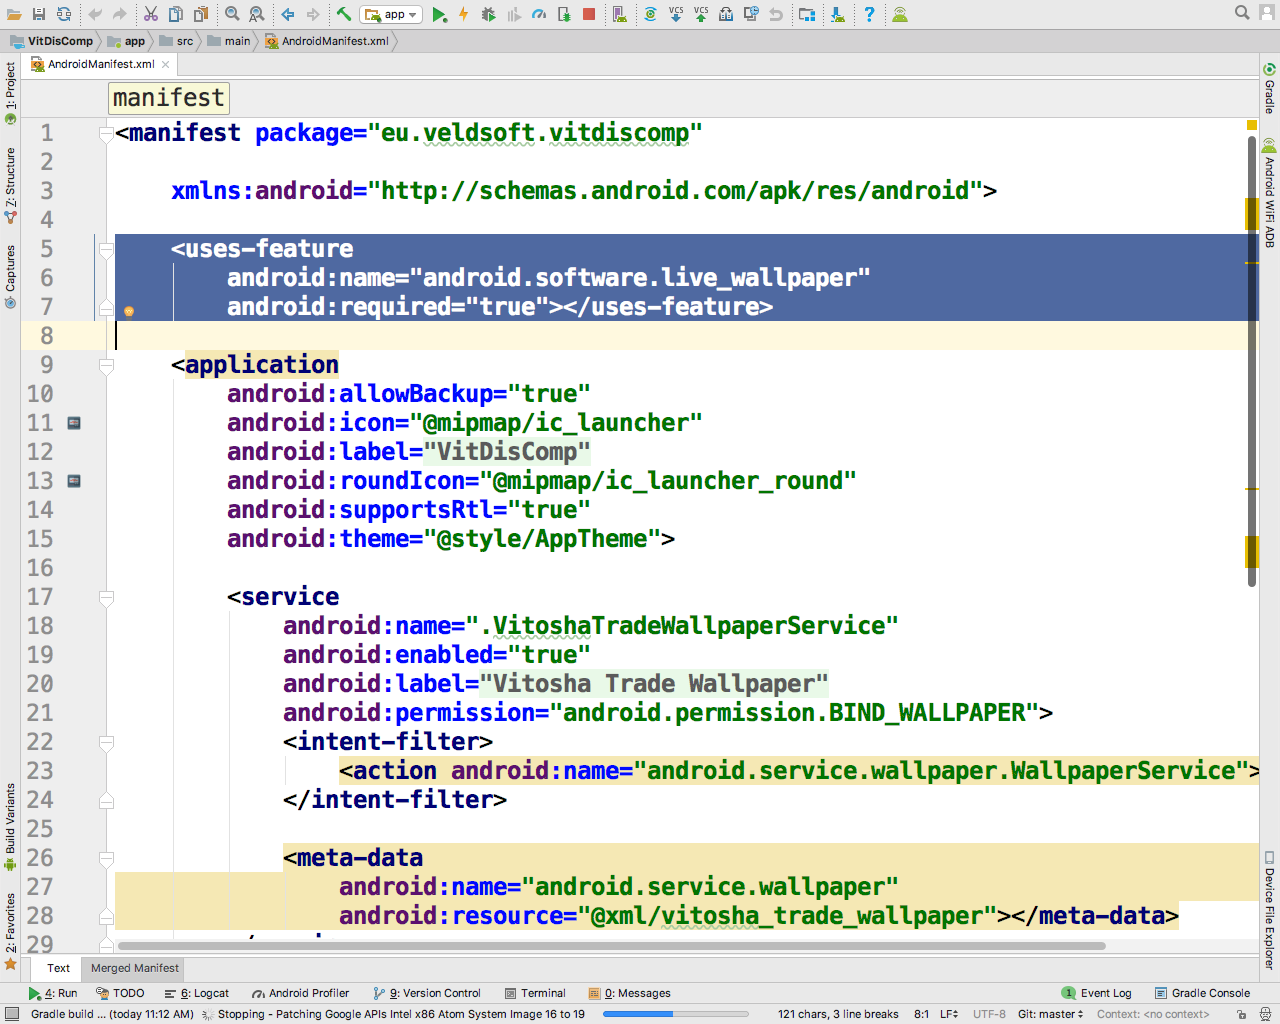
\includegraphics[height=0.45\pdfpageheight]{pic0011}
  \caption{Определяне на приложението като активен тапет}
\label{fig:pic0011}
\end{figure}
\FloatBarrier

За да се определи приложението като приложение от тип активен тапет, е необходимо това изрично да се маркира в манифест файла (Фиг. \ref{fig:pic0011}). Най-съществената полза от тази дефиниция е, че тя предотвратява възможността приложението да бъде инсталирано на устройства, които не поддържат възможностите за визуално представяне на активен тапет. 

\begin{figure}[h]
  \centering
  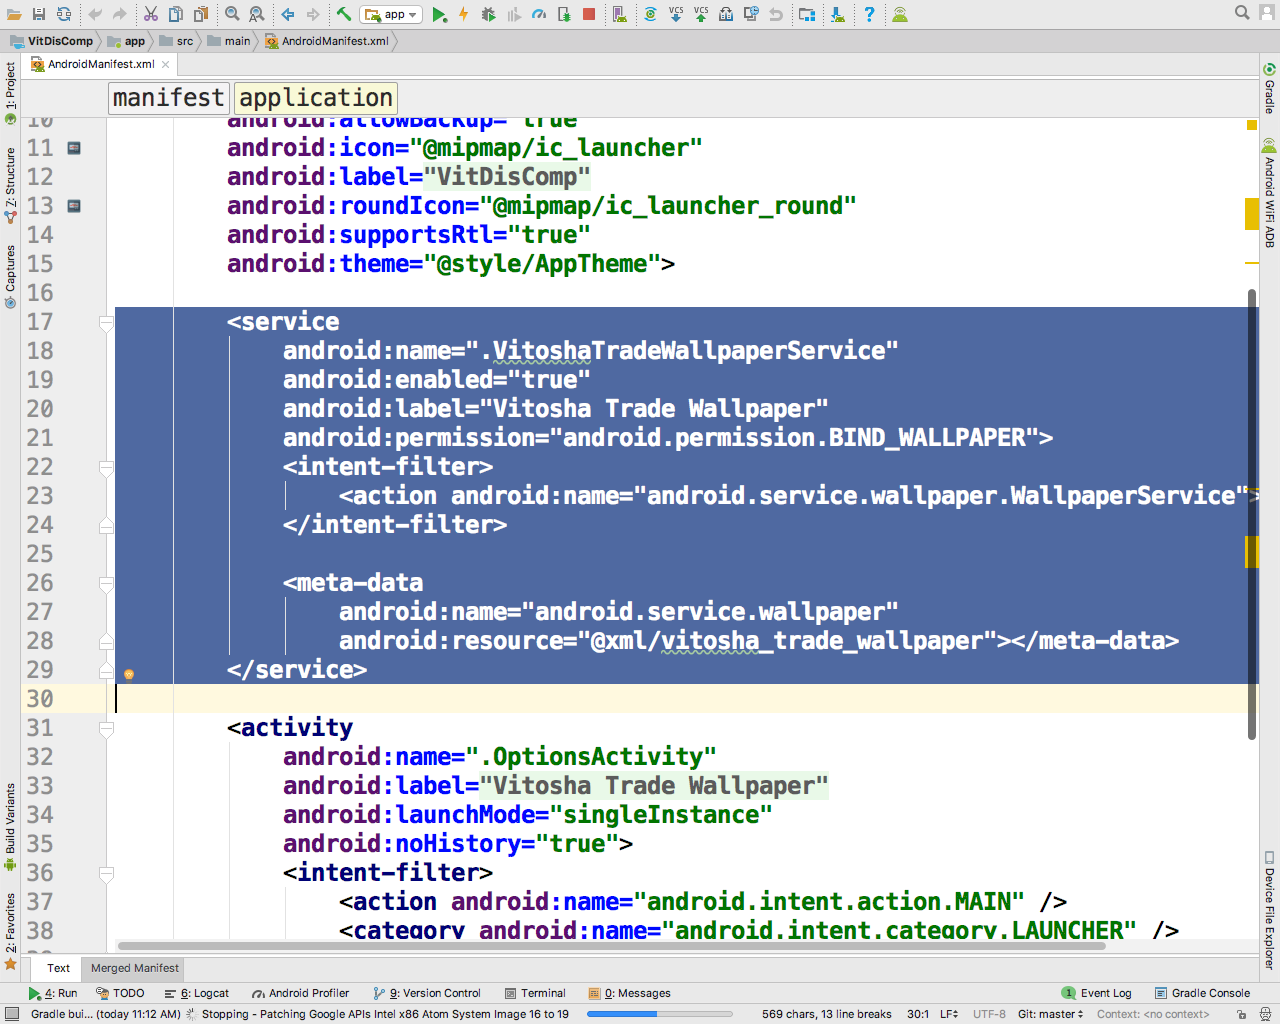
\includegraphics[height=0.45\pdfpageheight]{pic0012}
  \caption{Модул от тип ``услуга''}
\label{fig:pic0012}
\end{figure}
\FloatBarrier

Когато в Android се използват много продължителни пресмятания, които не са удачни за извършване, в нишка е прието тези изчисления да се изнасят в модули без графичен потребителски интерфейс, наречени „услуги“ (Service). Работата на активния тапет се извършва точно в такъв модул и поради тази причина в проекта е добавен един (Фиг. \ref{fig:pic0012}).

\begin{figure}[h]
  \centering
  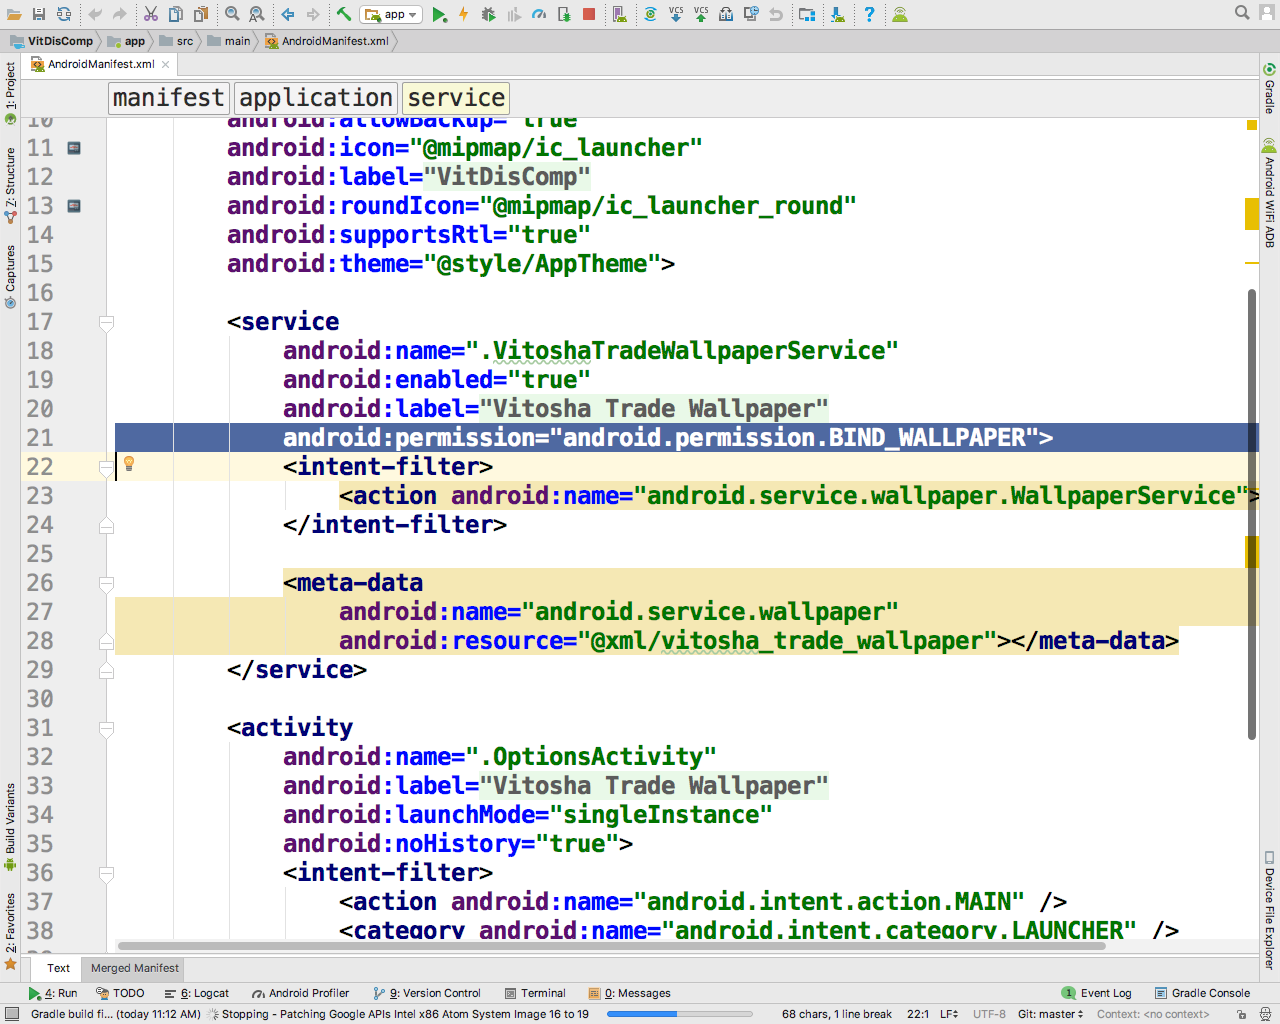
\includegraphics[height=0.45\pdfpageheight]{pic0013}
  \caption{Флагове за достъп до ресурса активен тапет}
\label{fig:pic0013}
\end{figure}
\FloatBarrier

Моделът за сигурност изисква за всяко по-особено действие да се получи изричното съгласие на потребителя. В случая с активния тапет е необходимо добавянето на android.permission.BIND\_WALLPAPER разрешение (Фиг. \ref{fig:pic0013}).

\begin{figure}[h]
  \centering
  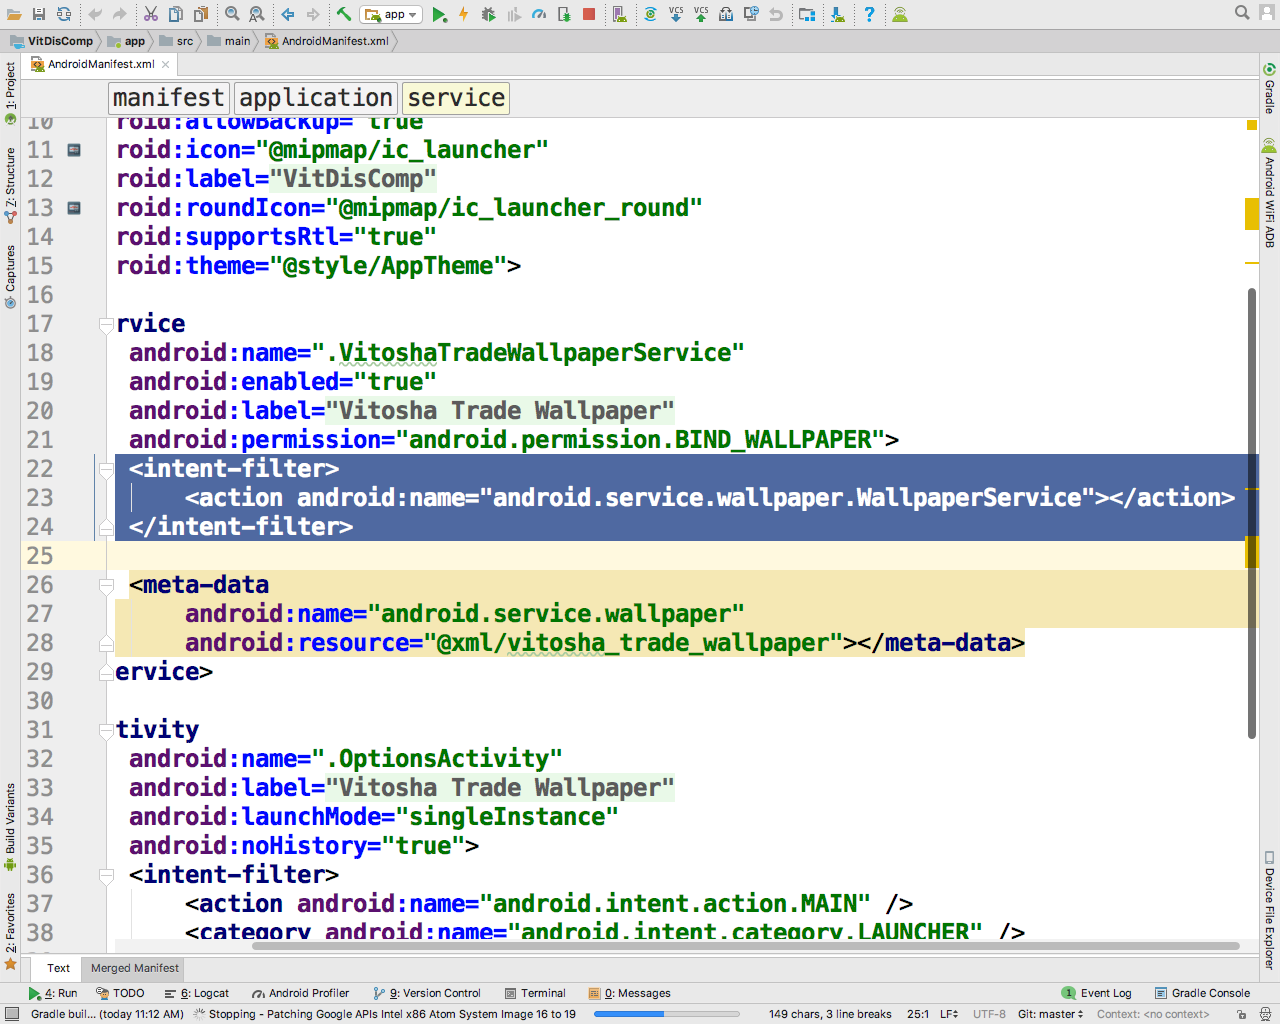
\includegraphics[height=0.45\pdfpageheight]{pic0014}
  \caption{Регистрация на услугата за прослушване на съобщения от операционната система.}
\label{fig:pic0014}
\end{figure}
\FloatBarrier

Освен нуждата от разрешения за ползване на ресурсите за активен тапет, е нужно услугата да се абонира за прослушване на съобщения от операционната система (Фиг. \ref{fig:pic0014}).

\begin{figure}[h]
  \centering
  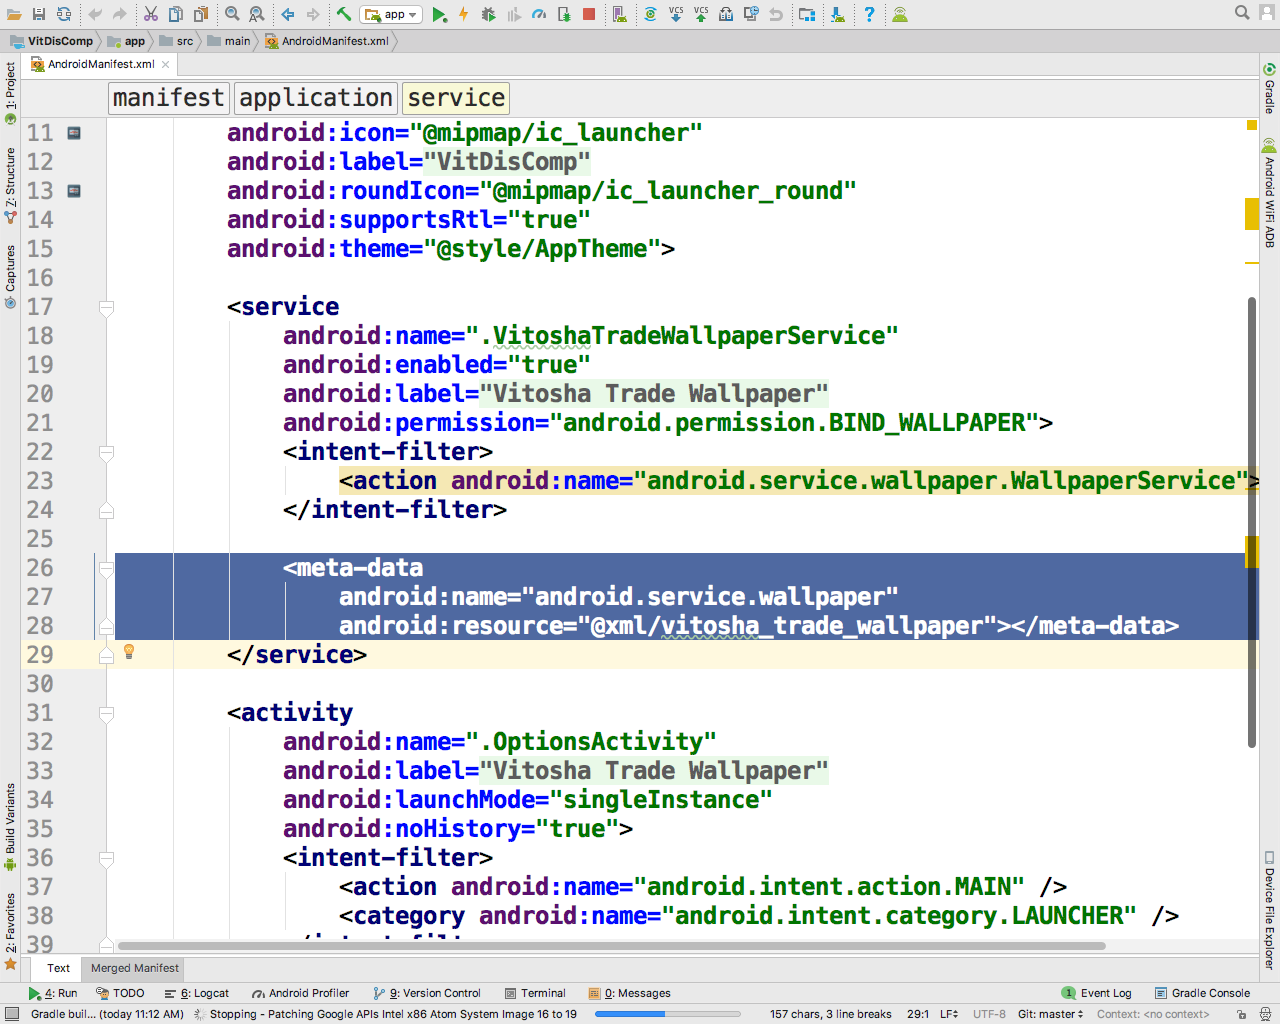
\includegraphics[height=0.45\pdfpageheight]{pic0015}
  \caption{Референция към описателния файл на активния тапет}
\label{fig:pic0015}
\end{figure}
\FloatBarrier

Описанието на самия активен тапет се съдържа в отделен XML файл, референция към който се посочва в манифеста (Фиг. \ref{fig:pic0015}).

\begin{figure}[h]
  \centering
  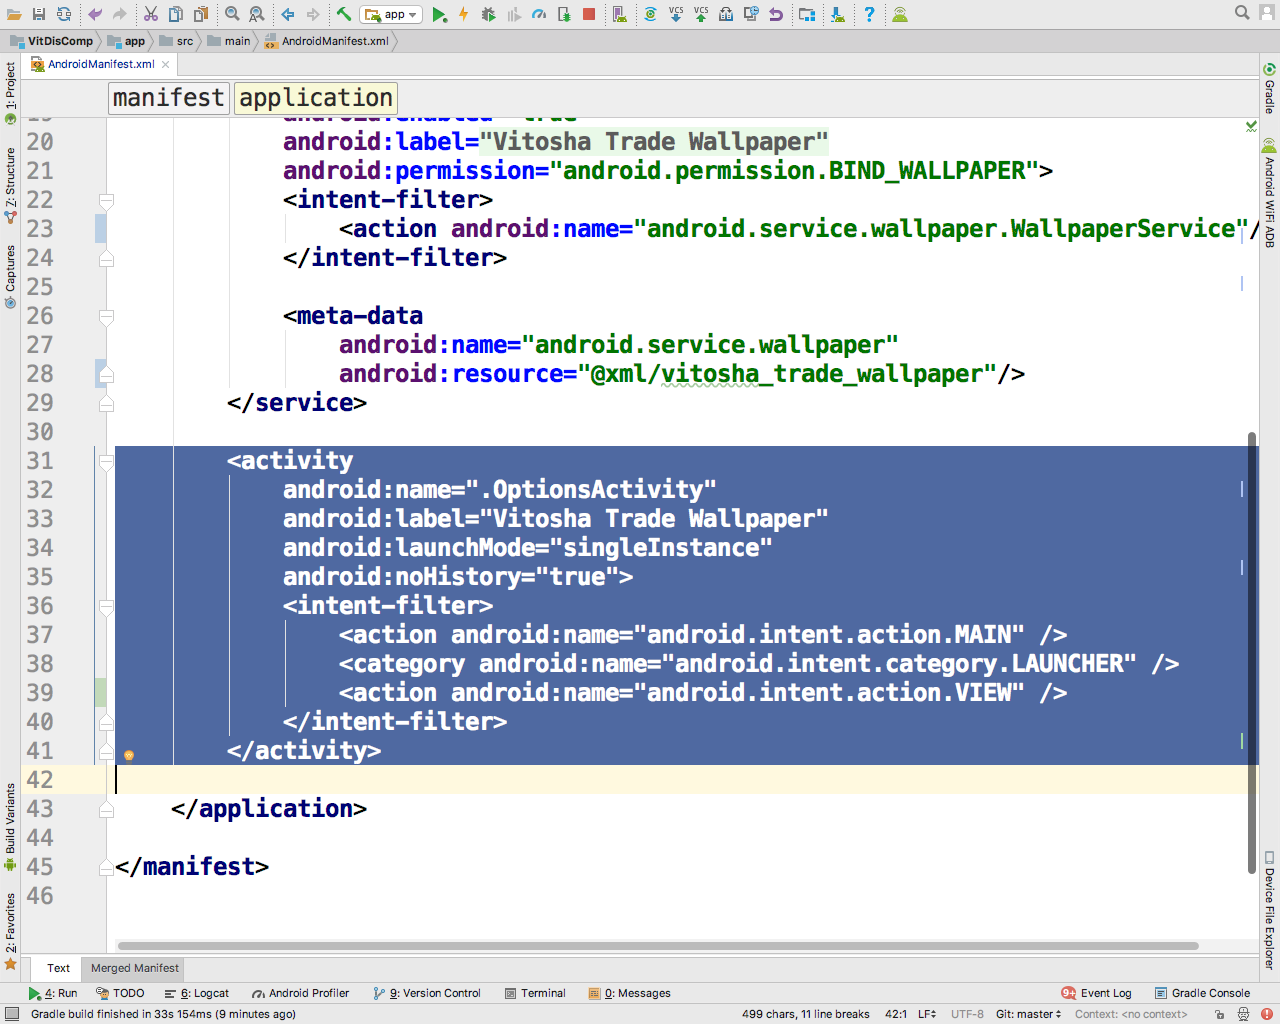
\includegraphics[height=0.45\pdfpageheight]{pic0016}
  \caption{Прозорец за установяване на активния тапет}
\label{fig:pic0016}
\end{figure}
\FloatBarrier

Последният компонент в такъв тип приложение е прозорец (Android Activity), който да се стартира от операционната система и да служи за установяване на активния тапет (Фиг. \ref{fig:pic0016}). В случая се използва възможността този стартов прозорец да съчетава и функциите на прозорец с опции (Preference Activity).

\begin{figure}[h]
  \centering
  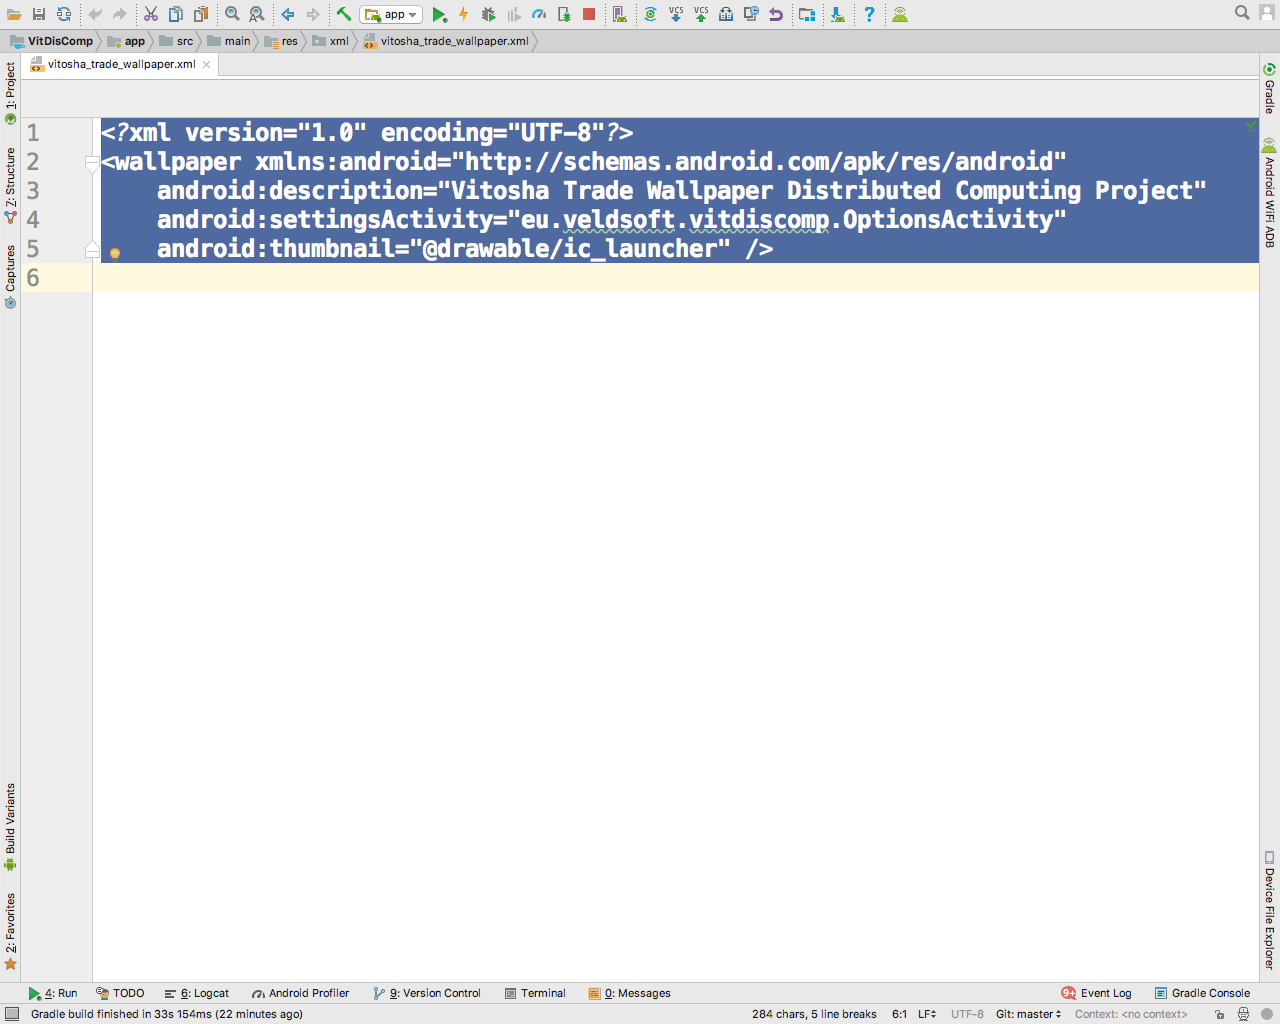
\includegraphics[height=0.45\pdfpageheight]{pic0017}
  \caption{XML описателен файл на тапета}
\label{fig:pic0017}
\end{figure}
\FloatBarrier

Както вече бе споменато, активният тапет се описва в отделен XML файл, който съдържа кратка анотация на приложението, предварителен изглед, умалена икона и името на прозореца за настройки (Фиг. \ref{fig:pic0017}). 

\section{Екран с настройки}

Тъй като активният тапет ще има и вторична задача да визуализира прогреса на пресмятанията, то е разумно към него да бъде създаден и прозорец с настройки. 

\begin{figure}[h]
  \centering
  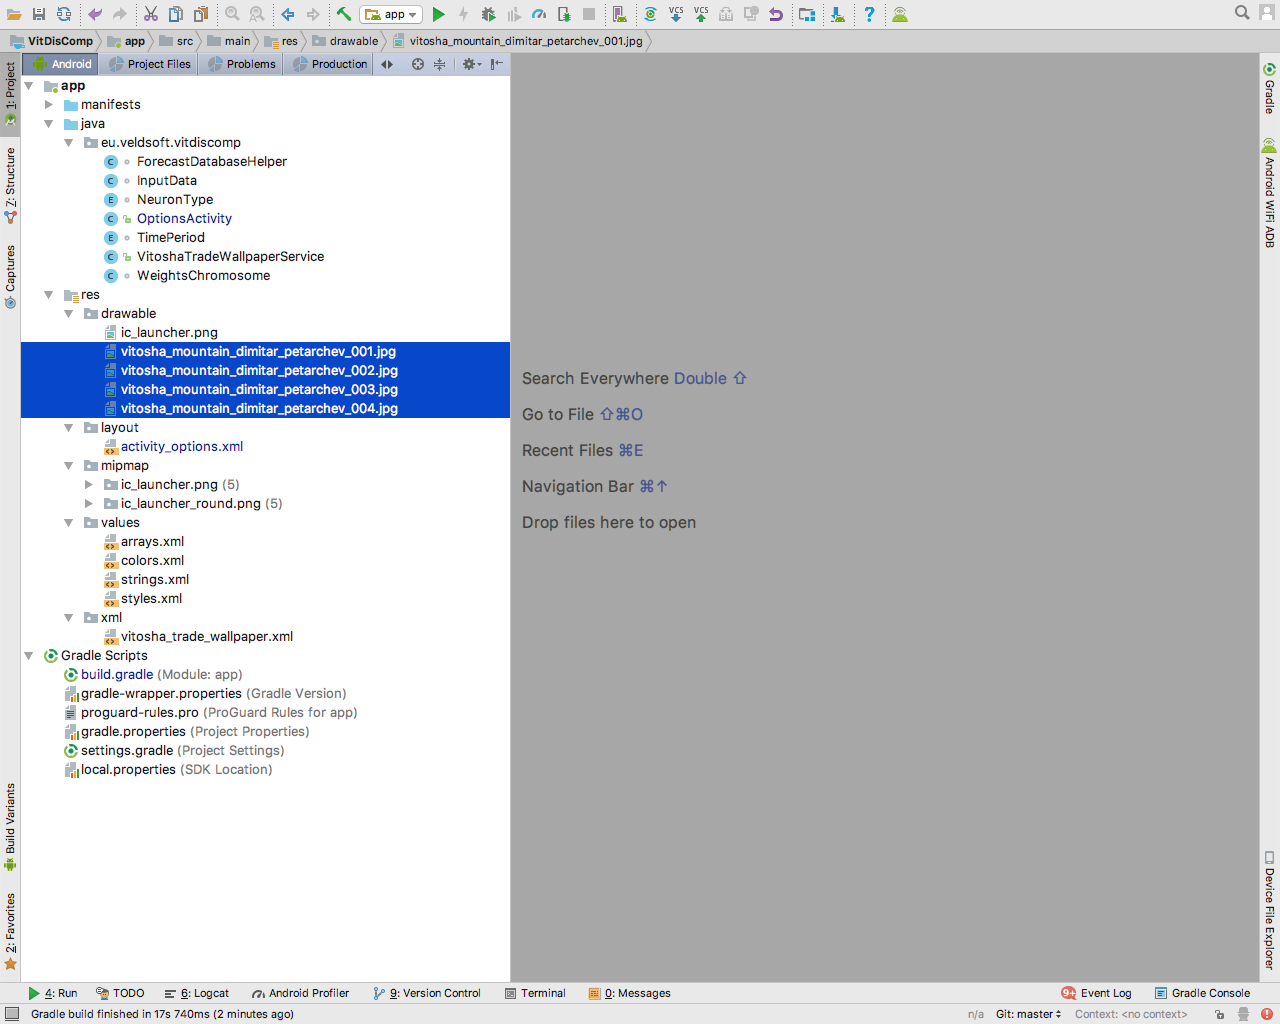
\includegraphics[height=0.45\pdfpageheight]{pic0018}
  \caption{Фотографии на планината Витоша до град София, България}
\label{fig:pic0018}
\end{figure}
\FloatBarrier

Като визуално представяне е избран възможно най-опростен вариант. Няколко фотографии на планината Витоша се визуализират под формата на отрязъци с размерите на екрана който мобилното устройство има (Фиг. \ref{fig:pic0018}). В три полупрозрачни области се визуализира информация за финансовия времеви ред (код и времеви период), стълб-диаграма за входните и изходните данни и текущо състояние на изкуствената невронна мрежа\index{изкуствени невронни мрежи} (Фиг. \ref{fig:pic0019}). 

\begin{figure}[h]
  \centering
  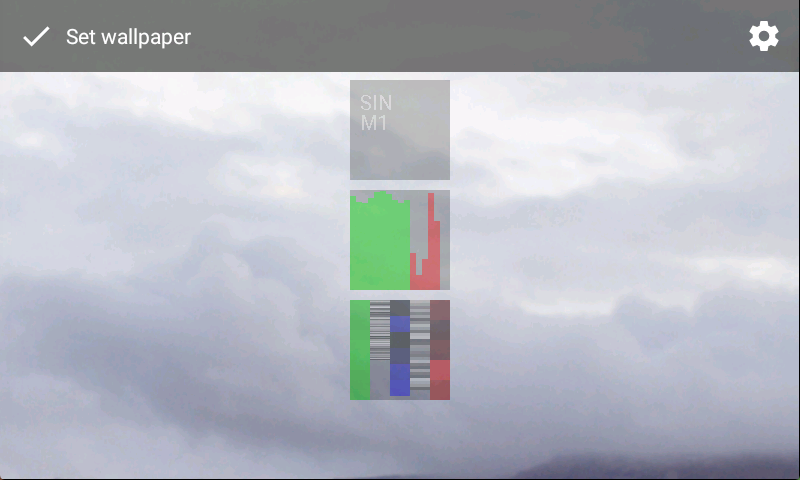
\includegraphics[width=1.0\linewidth]{pic0019}
  \caption{Висуално представяне на информация от изчисленията}
\label{fig:pic0019}
\end{figure}
\FloatBarrier

В настройките за активния тапет са предоставени възможности за управление на позицията и размерът за трите визуални области. Също така са добавени първоначални настройки за натоварване на устройството и дали активният тапет да бъде включен (Фиг. \ref{fig:pic0020}). 

\begin{figure}[h]
  \centering
  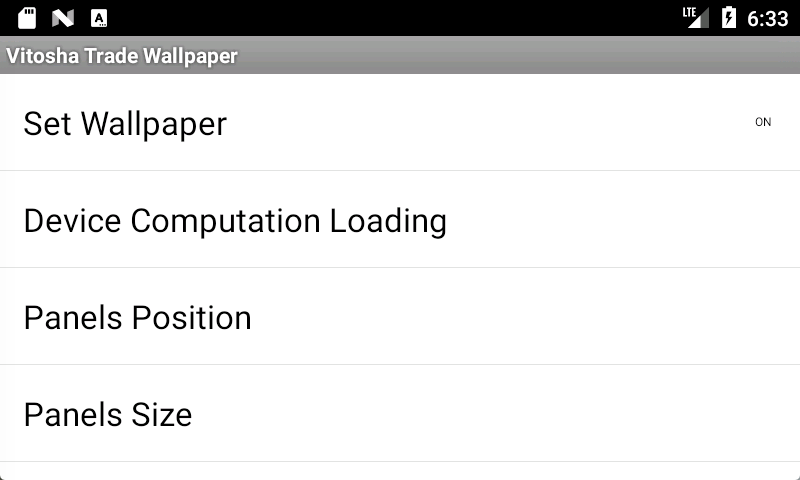
\includegraphics[width=1.0\linewidth]{pic0020}
  \caption{Първоначален набор от настройки}
\label{fig:pic0020}
\end{figure}
\FloatBarrier

Всеки прозорец в Android се описва със свой файл за разполагане (layout) и файл с Java програмен код. Описателният файл за графичен потребителски интерфейс използва XML и много наподобява съставянето на уеб страница. Когато се изготвя екран за настройки един от най-полезните инструменти в операционната система Android са споделените преференции (Shared Preferences). Те позволяват състоянието на визуалните компоненти директно да бъде запаметено в устройството под формата на ключ-стойност двойки и след това програмно тази информация да бъде използвана. 

\subsection{Описание на потребителския интерфейс под формата на XML файлове}

\begin{figure}[h]
  \centering
  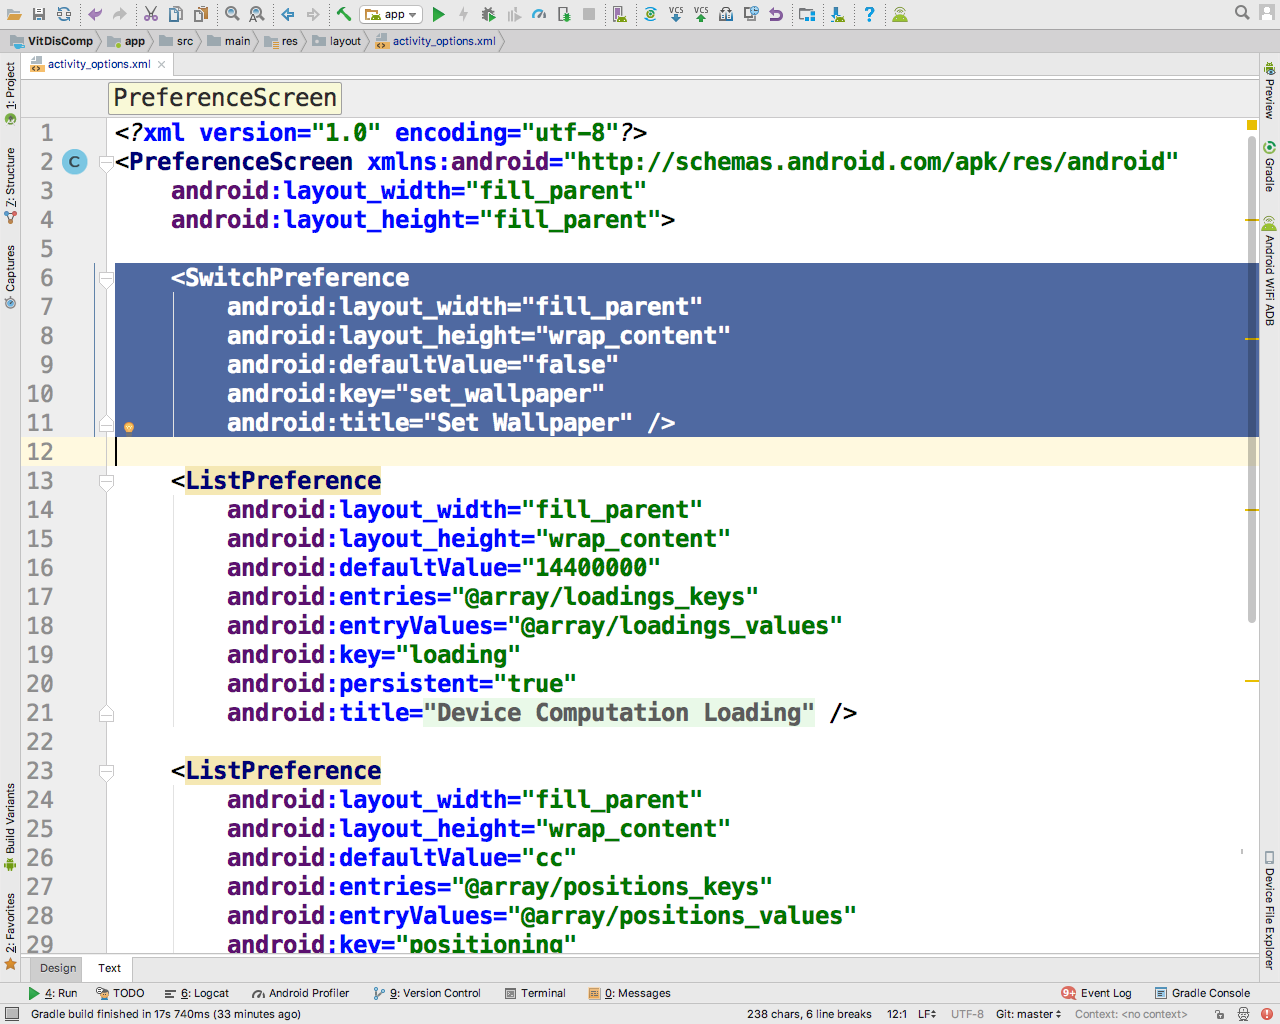
\includegraphics[height=0.45\pdfpageheight]{pic0021}
  \caption{Визуален компонент за включване и изключване на тапета}
\label{fig:pic0021}
\end{figure}
\FloatBarrier

На първо място е разположен визуален компонент за включване и изключване на активния тапет. Когато ключът е в състояние O,N активният тапет бива стартиран, а когато е в позиция OFF, активният тапет бива деактивиран (Фиг. \ref{fig:pic0021}). 

\begin{figure}[h]
  \centering
  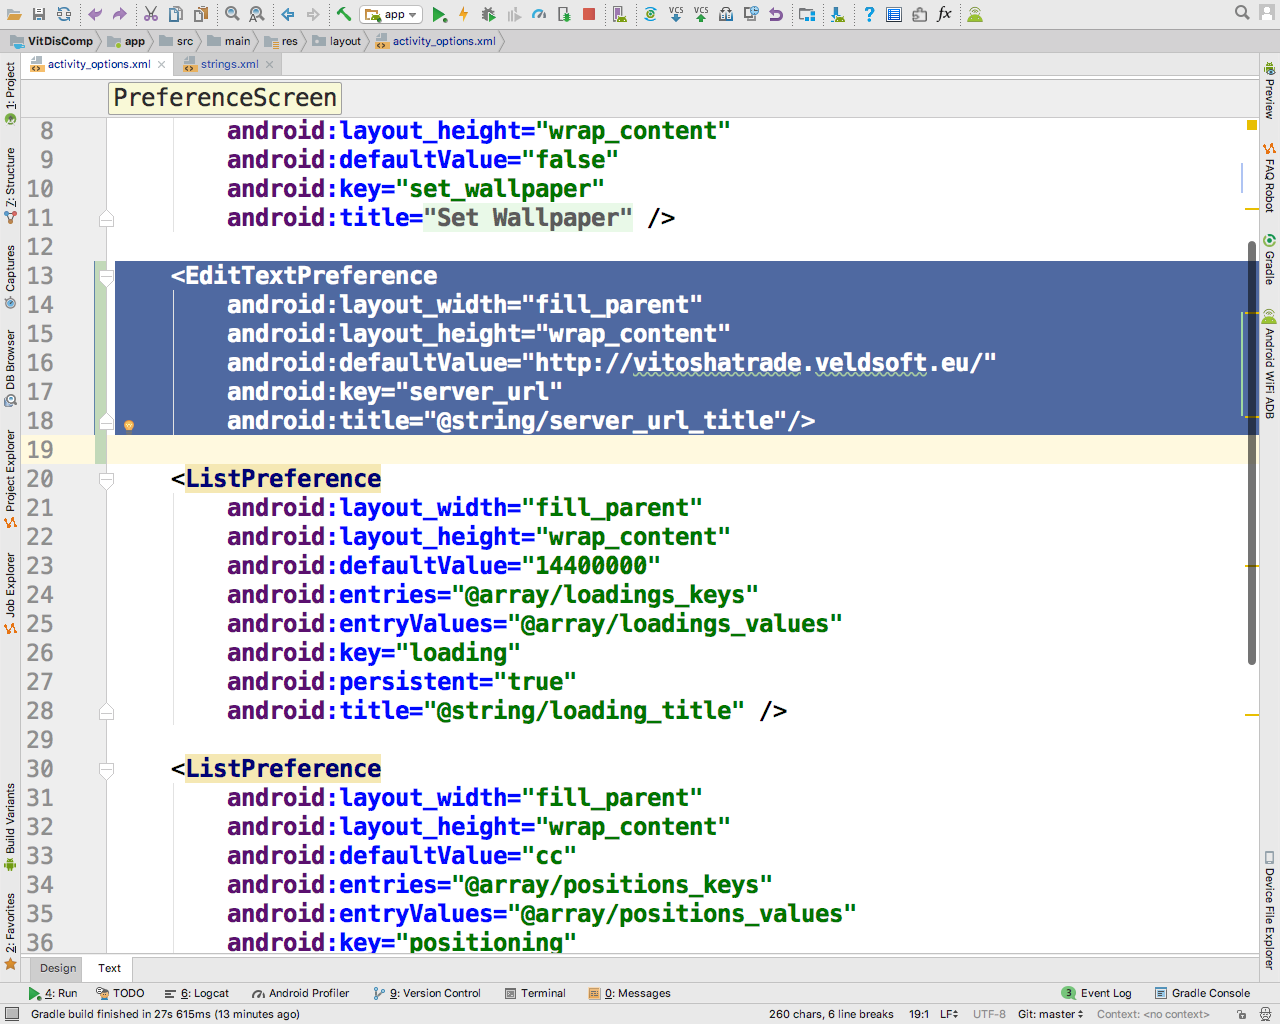
\includegraphics[height=0.45\pdfpageheight]{pic0154}
  \caption{Визуален компонент за посочване на сървър URL}
\label{fig:pic0154}
\end{figure}
\FloatBarrier

Тъй като мобилното приложение тегли информацията за времевите редове от отдалечен уеб сървър, то е подходящо потребителят да има възможност да настройва URL адреса на сървъра, с който се работи (Фиг. \ref{fig:pic0154}). Тази опция позволява пренасочване на трафика към други сървъри, след като мобилното приложение вече е инсталирано на потребителските мобилни устройства.

\begin{figure}[h]
  \centering
  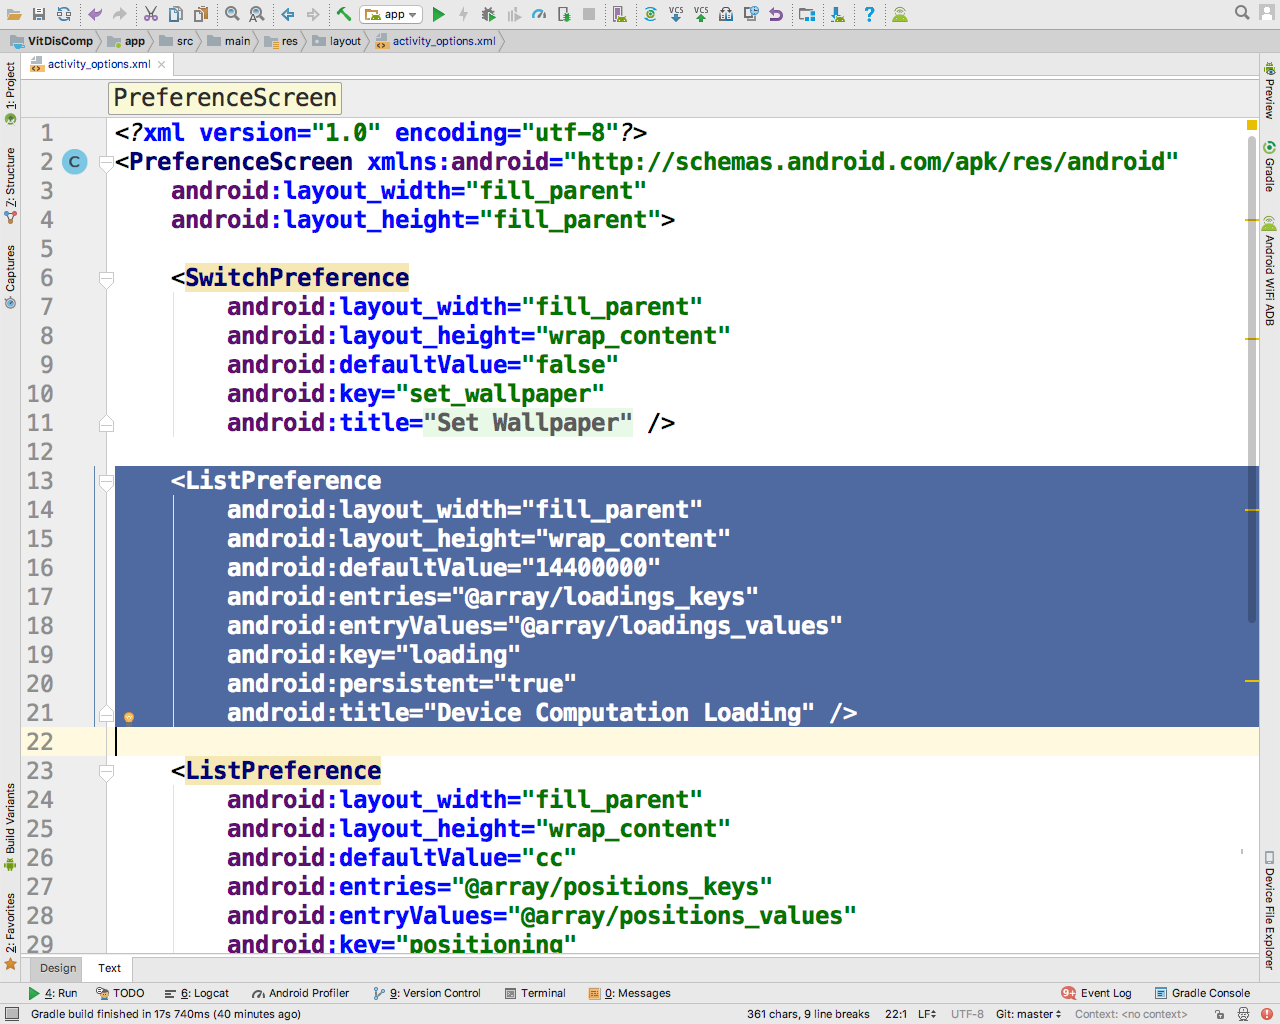
\includegraphics[height=0.45\pdfpageheight]{pic0022}
  \caption{Визуален компонент за регулиране на натоварването}
\label{fig:pic0022}
\end{figure}
\FloatBarrier

За натоварването на устройството при извършването на фоновите пресмятания се използва списък с предварително дефинирани стойности (Фиг. \ref{fig:pic0022}). 

\begin{figure}[h]
  \centering
  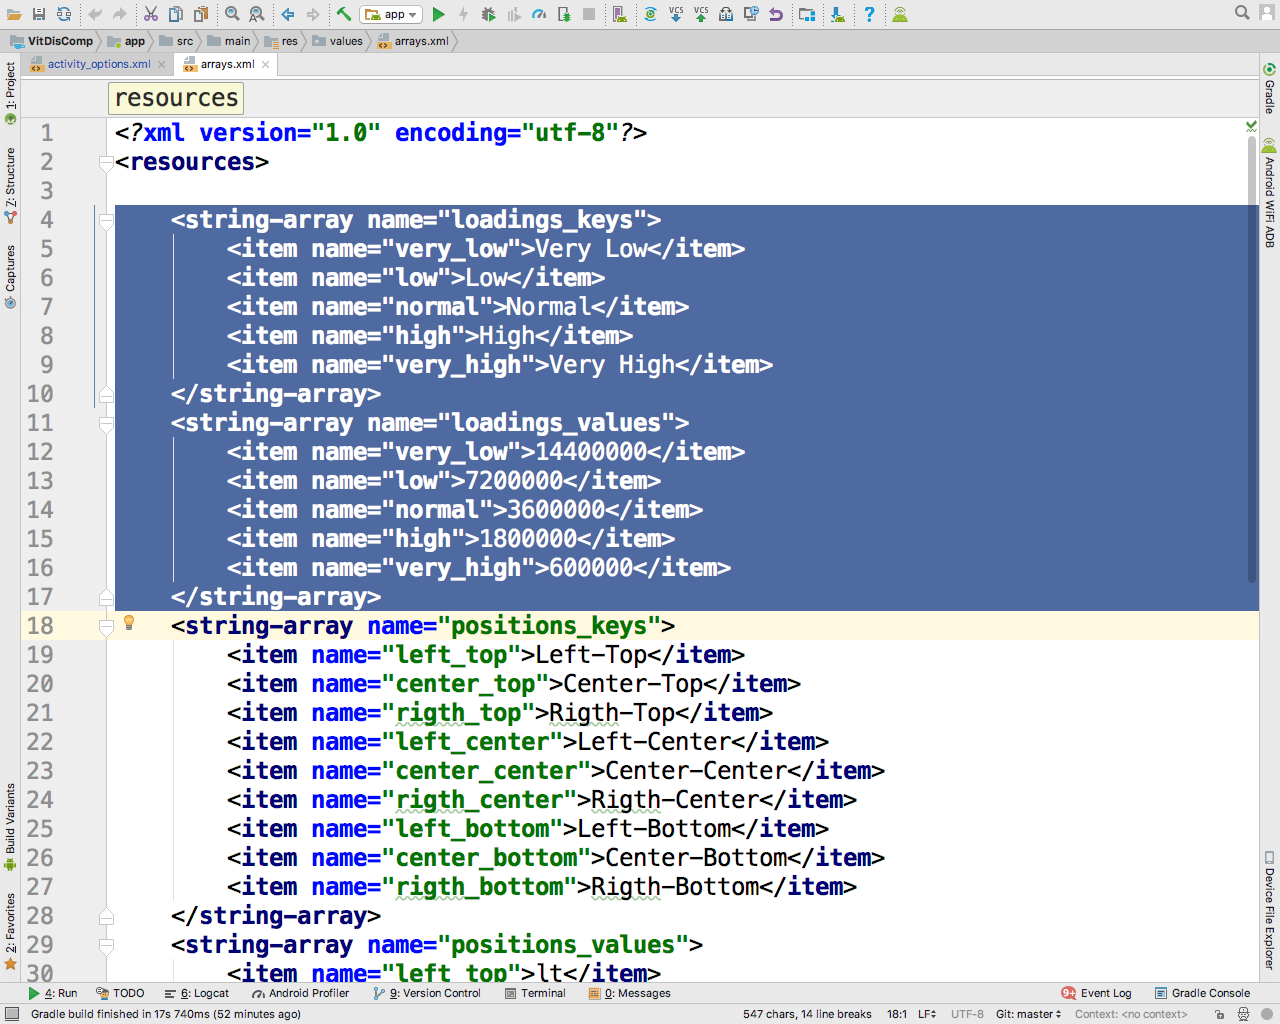
\includegraphics[height=0.45\pdfpageheight]{pic0023}
  \caption{Стойности за натоварване на системата}
\label{fig:pic0023}
\end{figure}
\FloatBarrier

При проектирането на системата Android, една от основните цели е била максимално разделяне на графичния интерфейс от данните. Точно поради тази причина стойностите за натоварване са изнесени в отделен ресурс (Фиг. \ref{fig:pic0023}).

\begin{figure}[h]
  \centering
  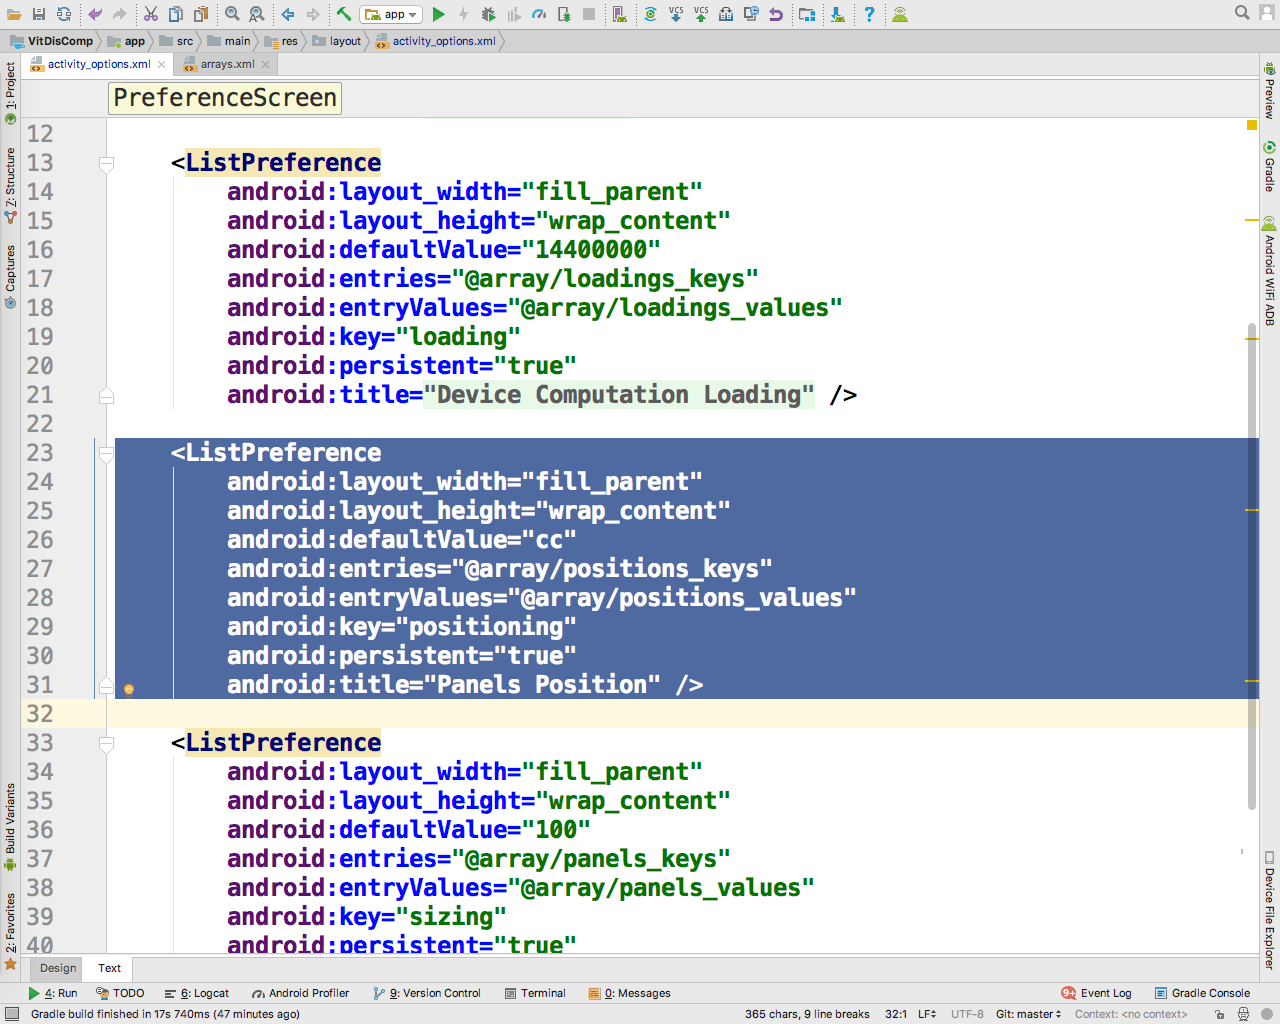
\includegraphics[height=0.45\pdfpageheight]{pic0024}
  \caption{Позициониране на областите за визуално представяне}
\label{fig:pic0024}
\end{figure}
\FloatBarrier

Позиционирането на областите за визуално представяне също се настройва с избор на стойности от списък (Фиг. \ref{fig:pic0024}). 

\begin{figure}[h]
  \centering
  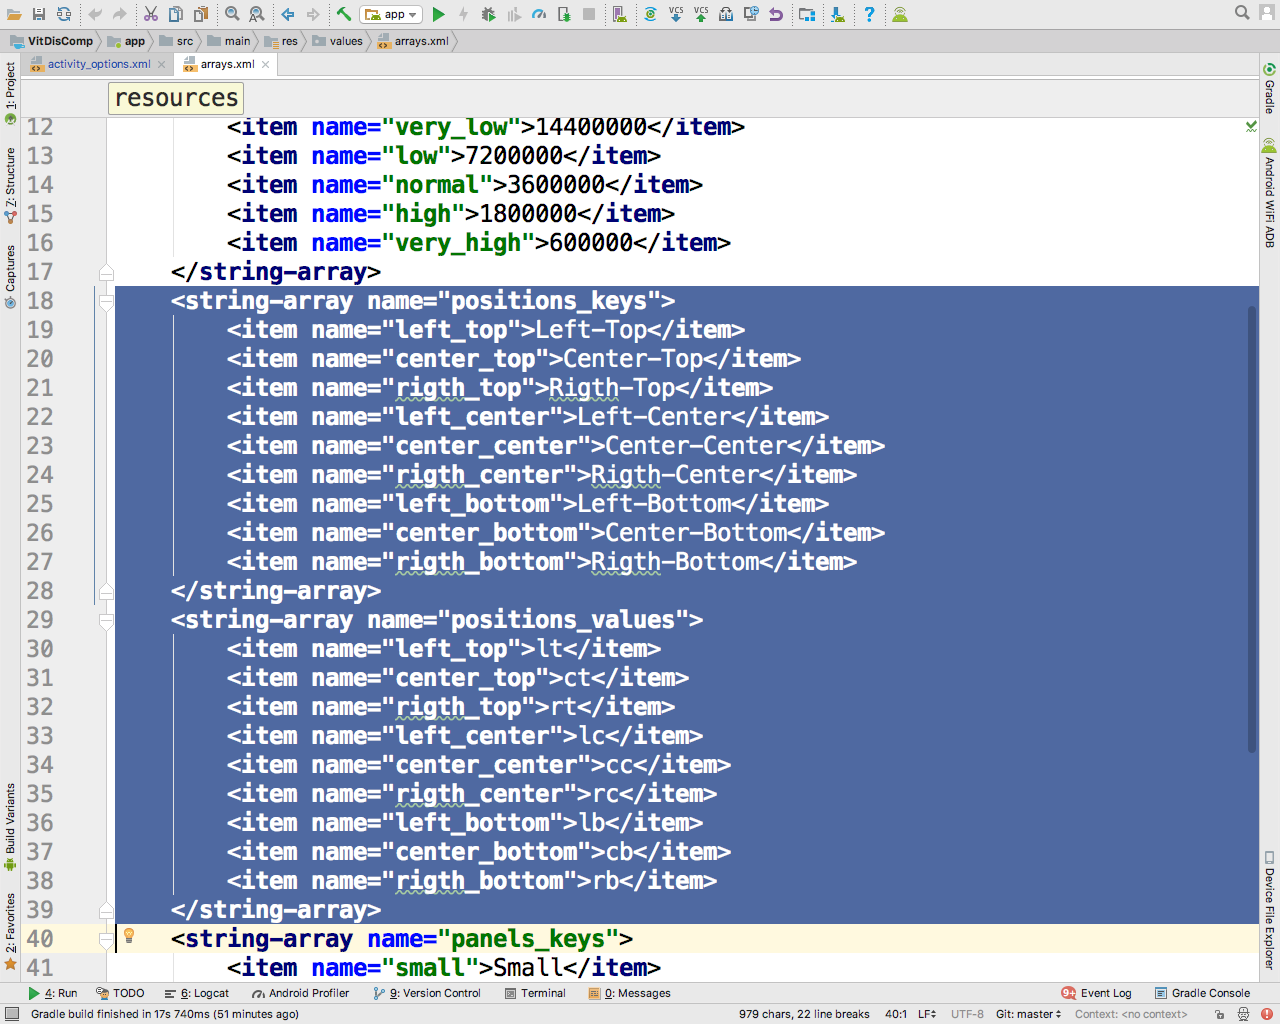
\includegraphics[height=0.45\pdfpageheight]{pic0025}
  \caption{Стойности за позициониране на областите за визуално представяне}
\label{fig:pic0025}
\end{figure}
\FloatBarrier

Аналогично на стойностите за натоварване, списъкът с възможните позиции на областите за визуално представяне е изнесен в отделен ресурсен файл (Фиг. \ref{fig:pic0025}). 

\begin{figure}[h]
  \centering
  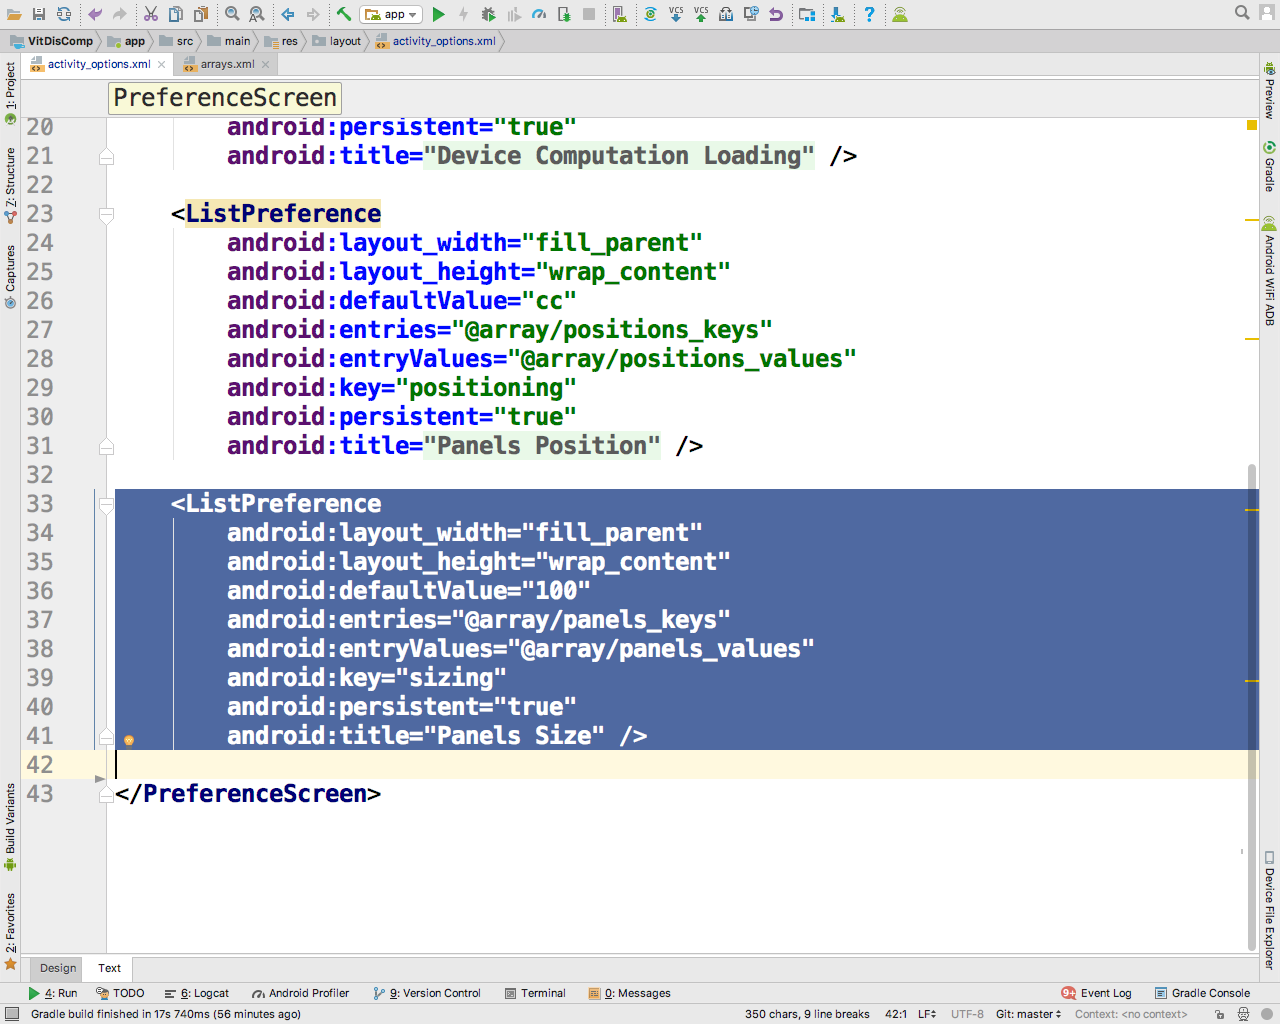
\includegraphics[height=0.45\pdfpageheight]{pic0026}
  \caption{Размер на областите за визуално представяне}
\label{fig:pic0026}
\end{figure}
\FloatBarrier

От първоначалните характеристики, последна е размерът на областите за визуално представяне на информацията (Фиг. \ref{fig:pic0026}). 

\begin{figure}[h]
  \centering
  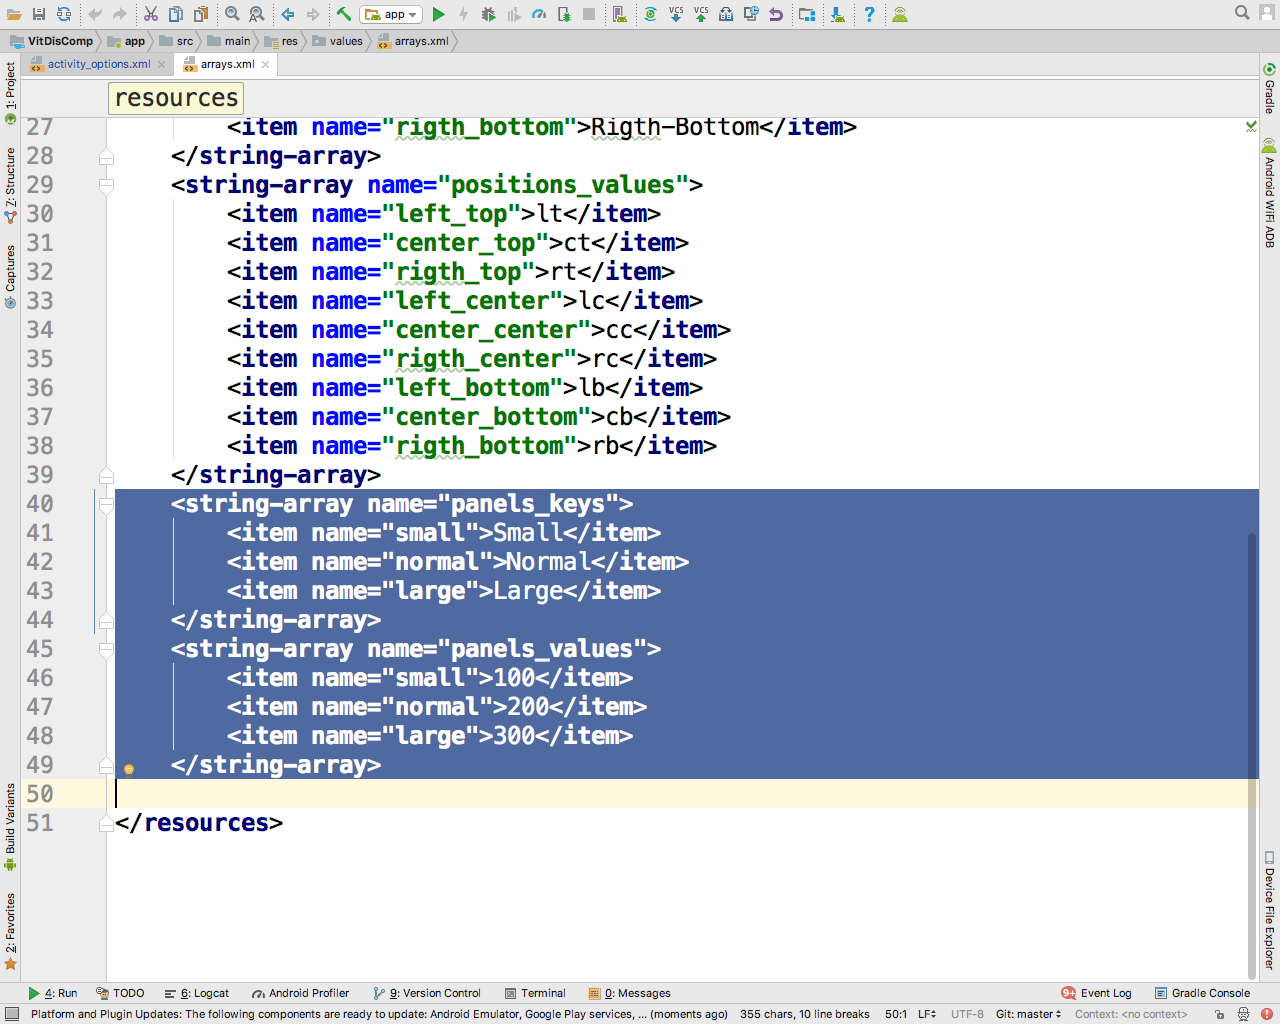
\includegraphics[height=0.45\pdfpageheight]{pic0027}
  \caption{Стойности за размер на областите за визуално представяне}
\label{fig:pic0027}
\end{figure}
\FloatBarrier

Областите за визуално представяне на информацията се предлагат в три размера – малък, среден и голям (Фиг. \ref{fig:pic0027}).

\subsection{Програмен код за управление на интерфейса}

Събитията, предизвикани от графичния програмен интерфейс, биват прихващани в специално написани за целта Java функции, така че при активирането им да бъдат извършени необходимите програмни действия. За екрана с настройки се прихващат само две събития – създаване и паузиране. 

\begin{figure}[h]
  \centering
  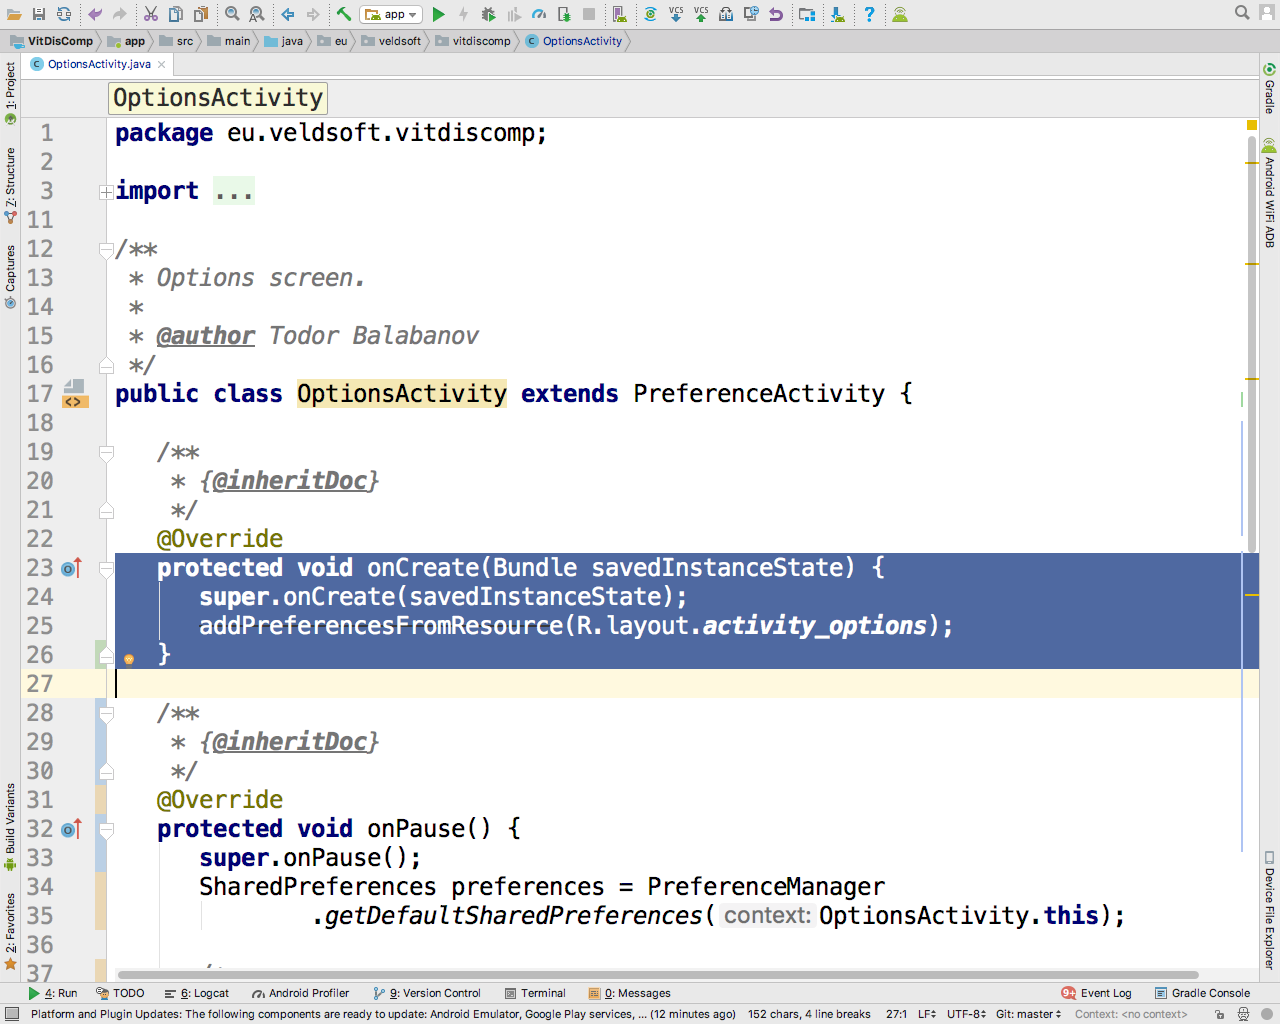
\includegraphics[height=0.45\pdfpageheight]{pic0028}
  \caption{Събитие за създаване на прозореца}
\label{fig:pic0028}
\end{figure}
\FloatBarrier

Събитието за създаване има за цел да трансформира XML описанието на интерфейса до визуални компоненти, видими за потребителя (Фиг. \ref{fig:pic0028}). 

\begin{figure}[h]
  \centering
  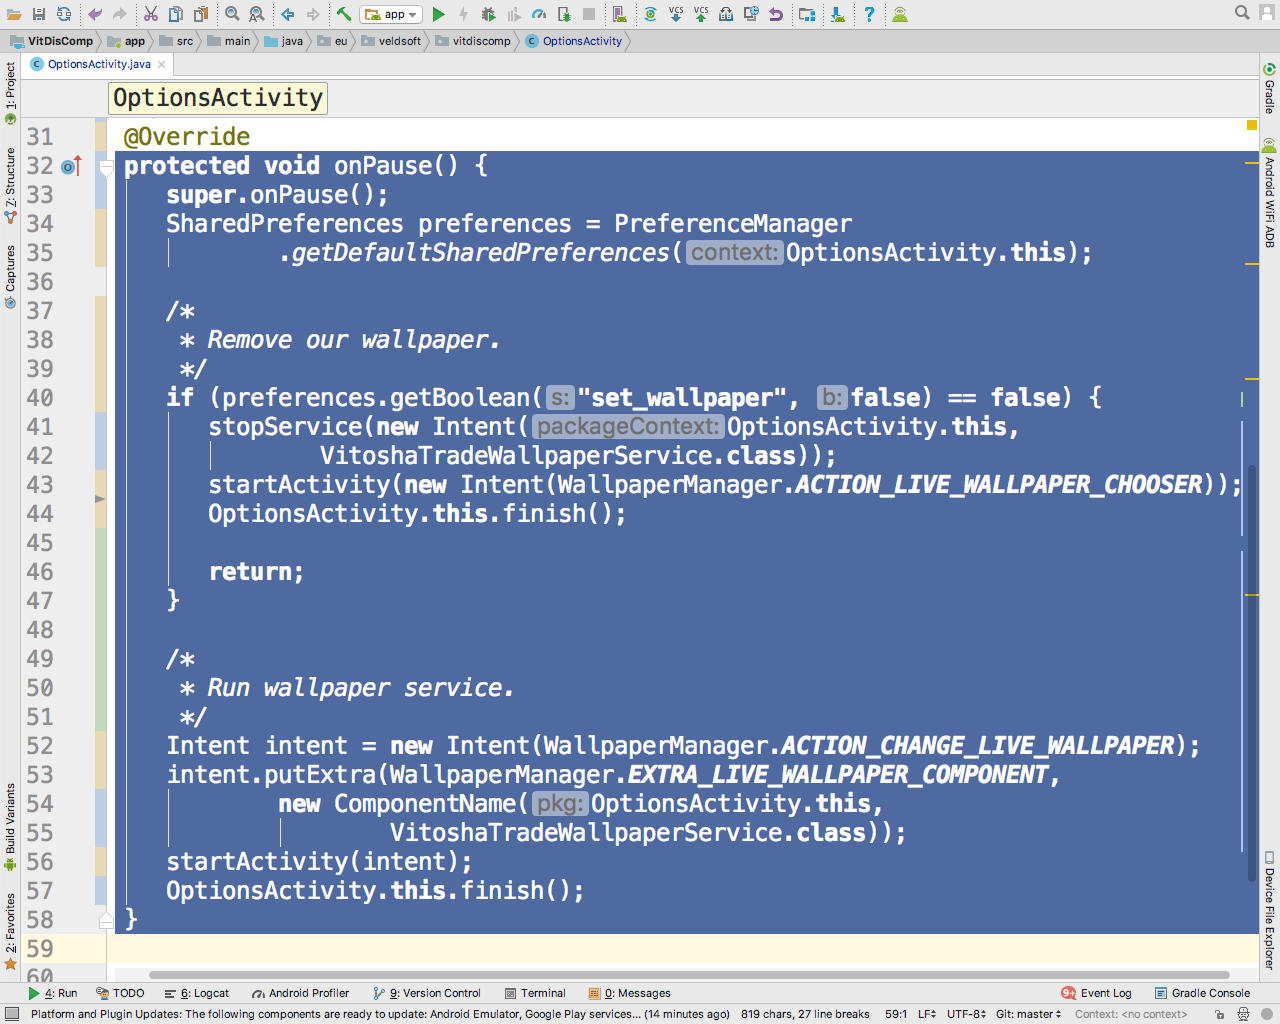
\includegraphics[height=0.45\pdfpageheight]{pic0029}
  \caption{Събитие за пауза на прозореца}
\label{fig:pic0029}
\end{figure}
\FloatBarrier

При събитието за пауза единствено се взема решение дали активният тапет да бъде стартиран или да бъде спрян (Фиг. \ref{fig:pic0029}). 

\section{Пресмятане на фонов режим}

Продължителните пресмятания, които не изискват графичен потребителски интерфейс се осъществяват в модули, наречени „услуги“ (Service). Когато става въпрос за активен тапет, е необходимо да се напише собствен клас, който е наследник на класа WallpaperService (Фиг. \ref{fig:pic0030}).

\begin{figure}[h]
  \centering
  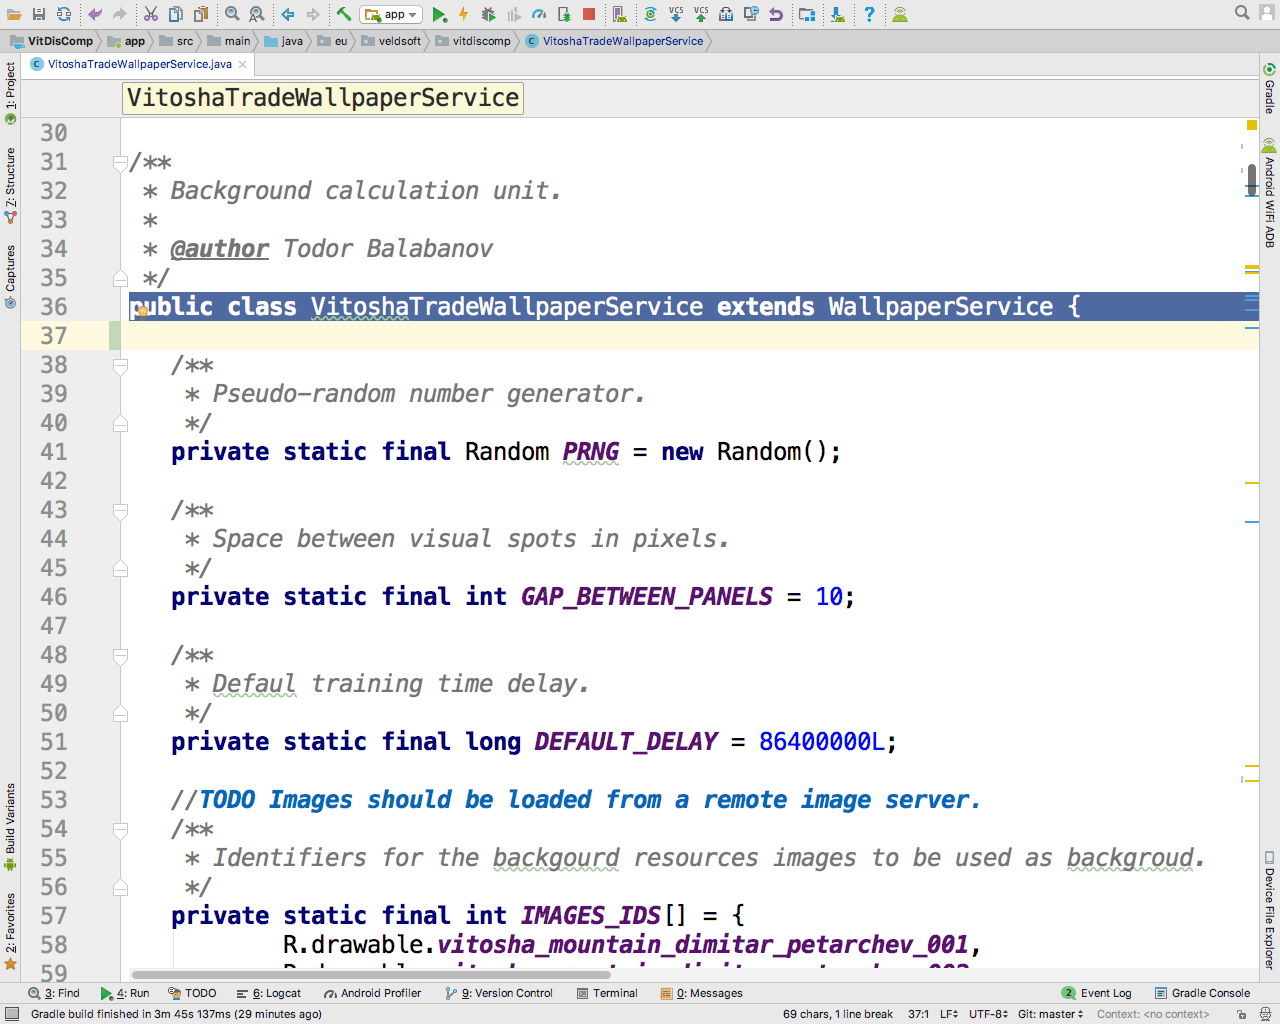
\includegraphics[height=0.45\pdfpageheight]{pic0030}
  \caption{Наследяване на WallpaperService}
\label{fig:pic0030}
\end{figure}
\FloatBarrier

Група от константи спомагат за генерирането на случайни числа, определяне на разстояние между зоните за визуално представяне и подразбираща се стойност за времето между две отделни стартирания на тренировъчния алгоритъм (Фиг. \ref{fig:pic0031}). 

\begin{figure}[h]
  \centering
  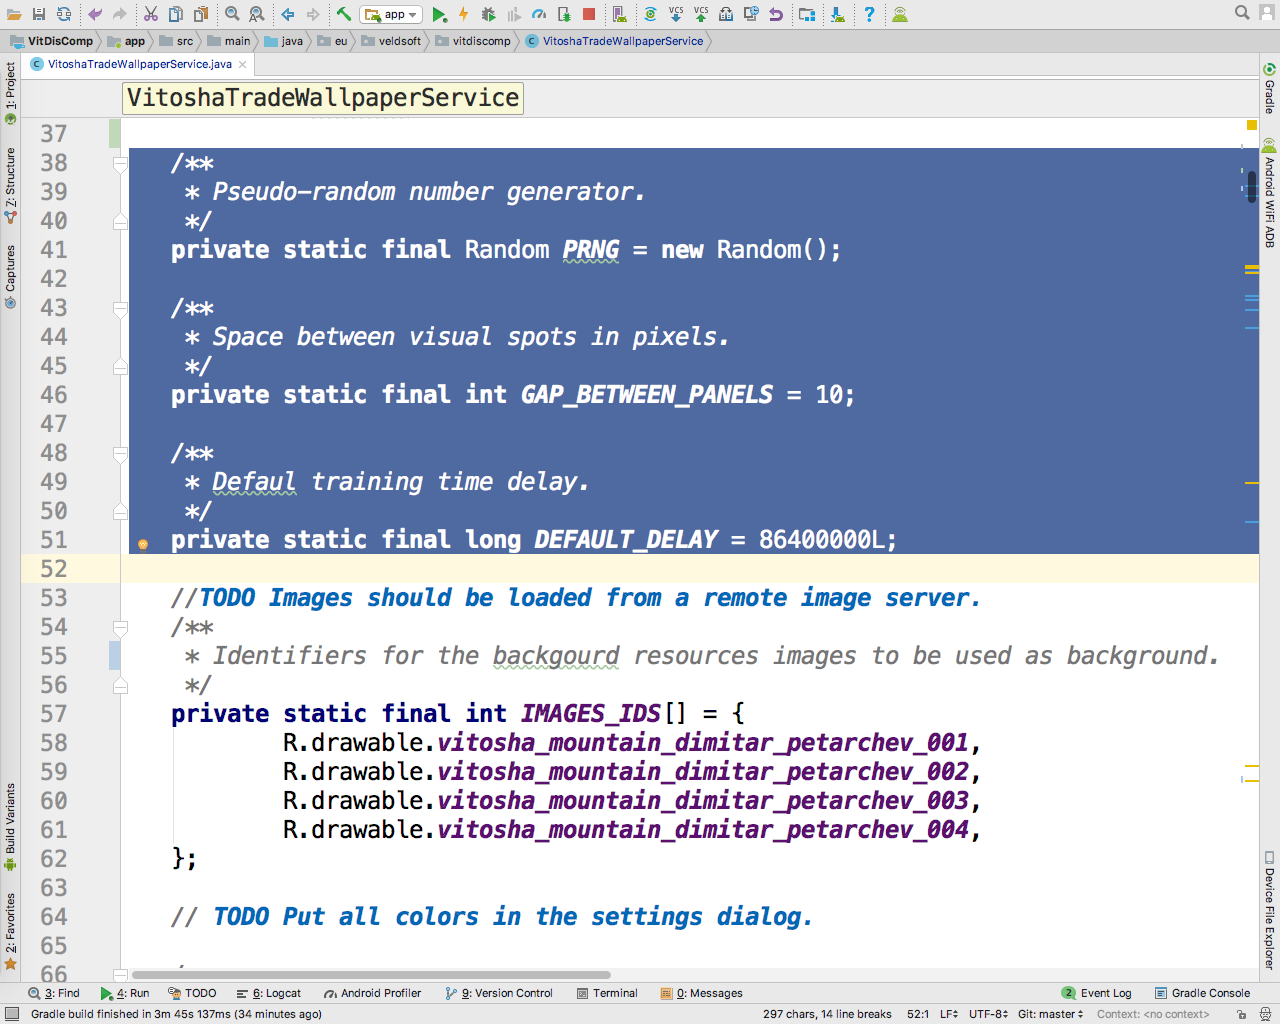
\includegraphics[height=0.45\pdfpageheight]{pic0031}
  \caption{Спомагателни константи}
\label{fig:pic0031}
\end{figure}
\FloatBarrier

Цветовете, използвани за визуалното представяне, също са зададени с група от константи, но в последствие ще бъдат превърнати в настройки със стойности от прозореца за настройки (Фиг. \ref{fig:pic0032}).

\begin{figure}[h]
  \centering
  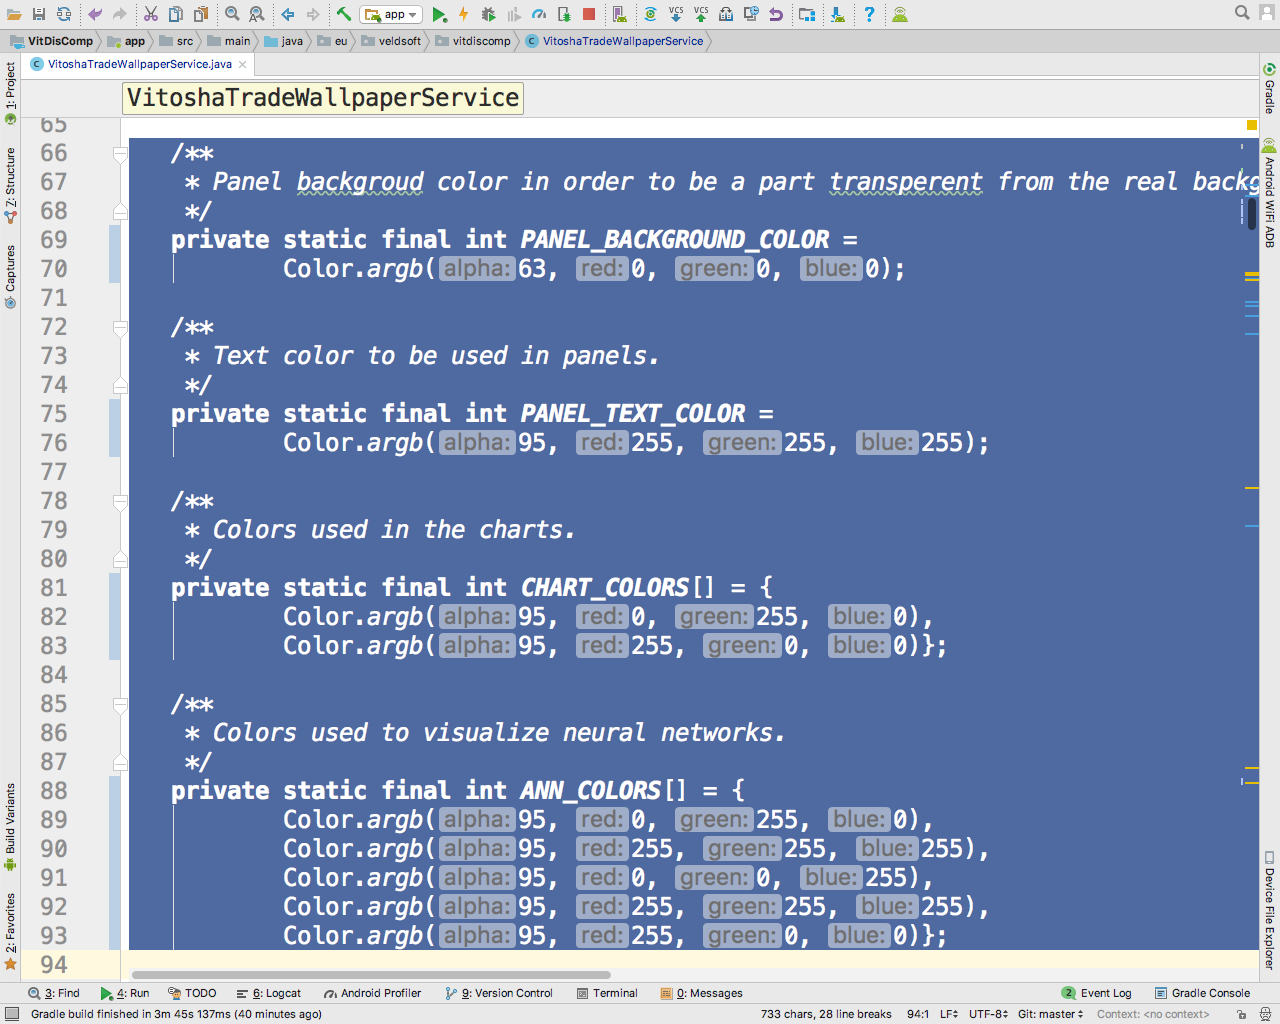
\includegraphics[height=0.45\pdfpageheight]{pic0032}
  \caption{Константи за цветовете}
\label{fig:pic0032}
\end{figure}
\FloatBarrier

Група променливи отговарят за състоянието на активния тапет. Това включва – размери на екрана, време между отделните обучения на изкуствената невронна мрежа, дали активният тапет е включен или изключен и точната позиция на зоните за визуално представяне на информацията от процеса по обучение на изкуствената невронна мрежа (Фиг. \ref{fig:pic0033}). 

\begin{figure}[h]
  \centering
  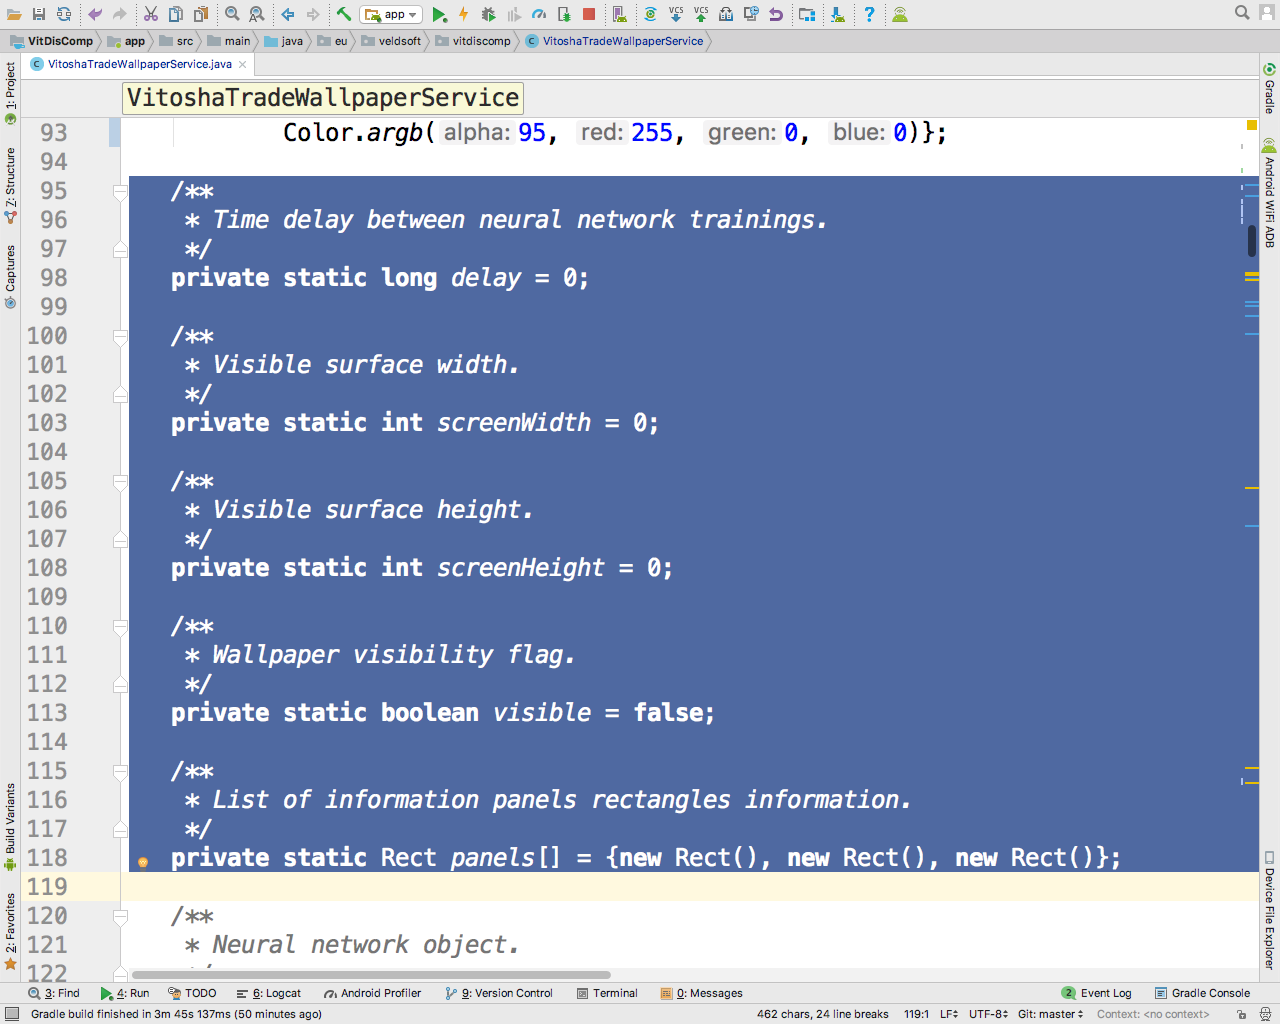
\includegraphics[height=0.45\pdfpageheight]{pic0033}
  \caption{Променливи отразяващи състоянието на активния тапет}
\label{fig:pic0033}
\end{figure}
\FloatBarrier

Друга група променливи (референции към обекти) поемат отговорността за управлението на изкуствената невронна мрежа, тренировъчните примери, входно-изходните данни към мрежата и правилото за нейното обучение (Фиг. \ref{fig:pic0034}).

\begin{figure}[h]
  \centering
  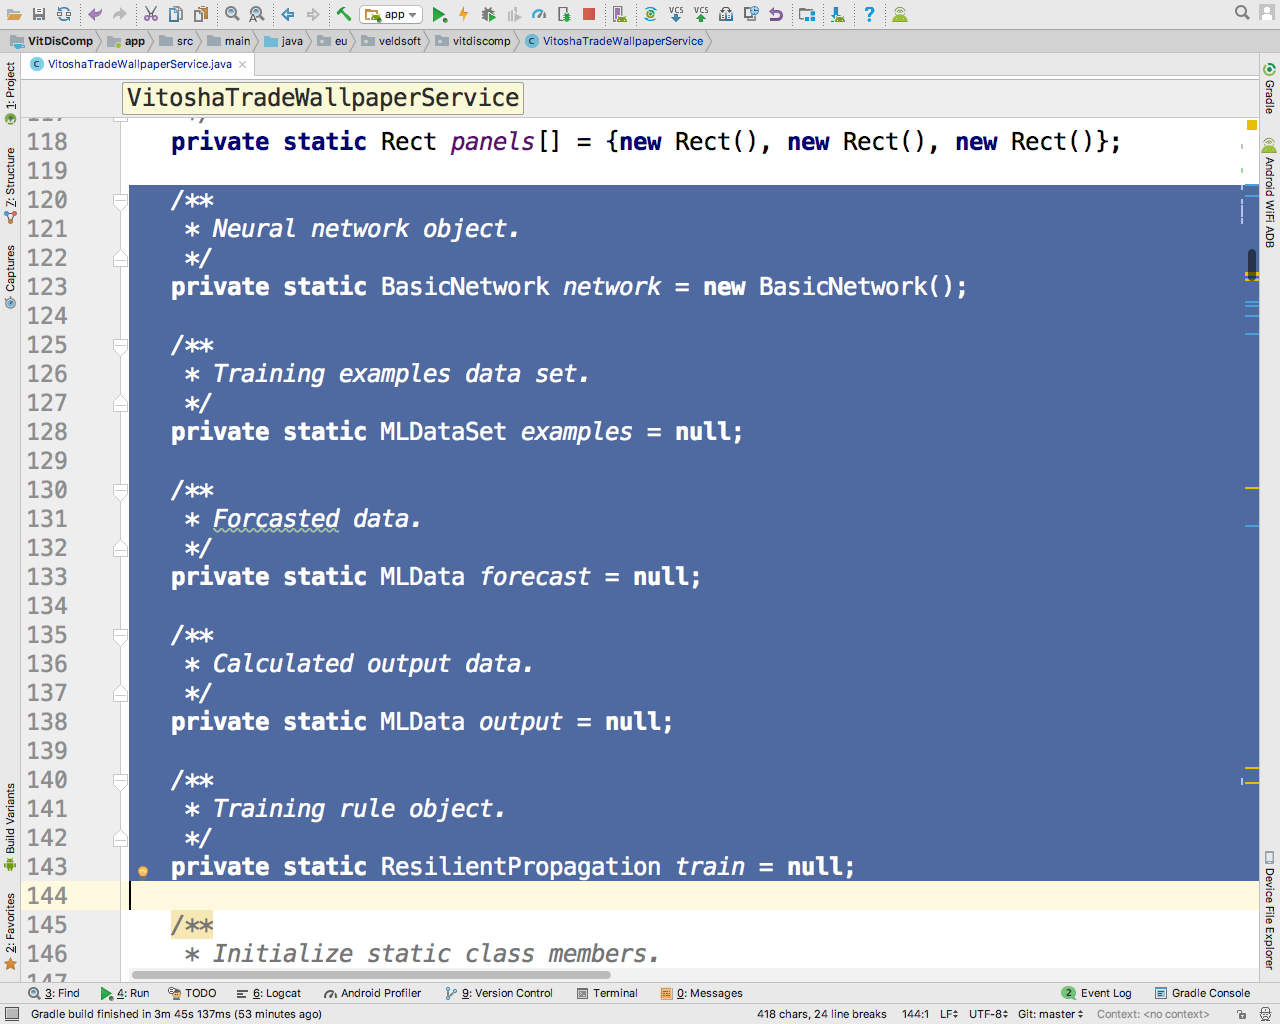
\includegraphics[height=0.45\pdfpageheight]{pic0034}
  \caption{Променливи отговарящи за изкуствената невронна мрежа}
\label{fig:pic0034}
\end{figure}
\FloatBarrier

При комерсиалното производство на софтуер много често използван похват е създаването на „софтуерни тапи“. Това са парчета код, които служат за комуникация между обекти и части от системата, които още не са създадени. В настоящия случай точно такава софтуерна тапа представя липсата на сървър и източник с реални данни  (Фиг. \ref{fig:pic0035}).  

\begin{figure}[h]
  \centering
  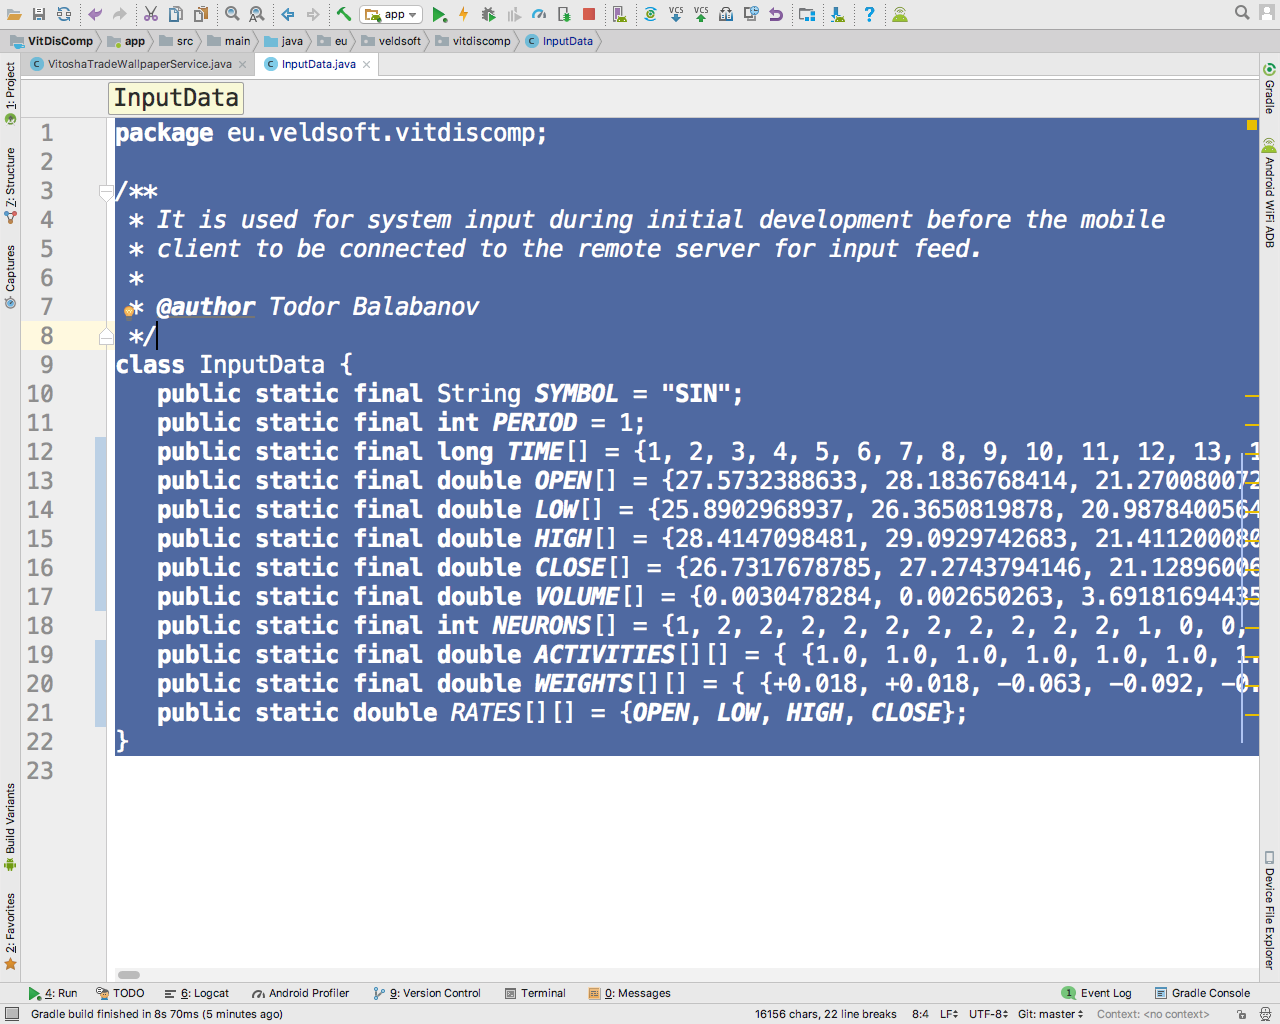
\includegraphics[height=0.45\pdfpageheight]{pic0035}
  \caption{Променливи отговарящи за изкуствената невронна мрежа}
\label{fig:pic0035}
\end{figure}
\FloatBarrier

Финансовите времеви редове най-често се описват със следните характеристики: 1. Вид финансов инструмент (ticker symbol или stock symbol), в случая математическата функция синус; 2. Интервал между отделните измервания (отчитан в брой минути), в случая една минута; 3. Шест паралелни масива (дискретно време, нива на отваряне, най-ниско постигнато ниво, най-високо постигнато ниво, нива на затваряне и изтъргуван обем).

Освен финансовата информация, към клиентското приложение трябва да се подава и информация за топологията на изкуствената невронна мрежа. За описанието на изкуствената невронна мрежа са нужни: 1. Брой, подредба и тип на невроните (едномерен масив от константи); 2. Матрица на съседство между невроните (единица там, където има връзка и нула там, където няма връзка); 3. Текуща стойност на тегловния коефициент за всяка връзка между два неврона (включително и примките, ако има такива). 

\begin{figure}[h]
  \centering
  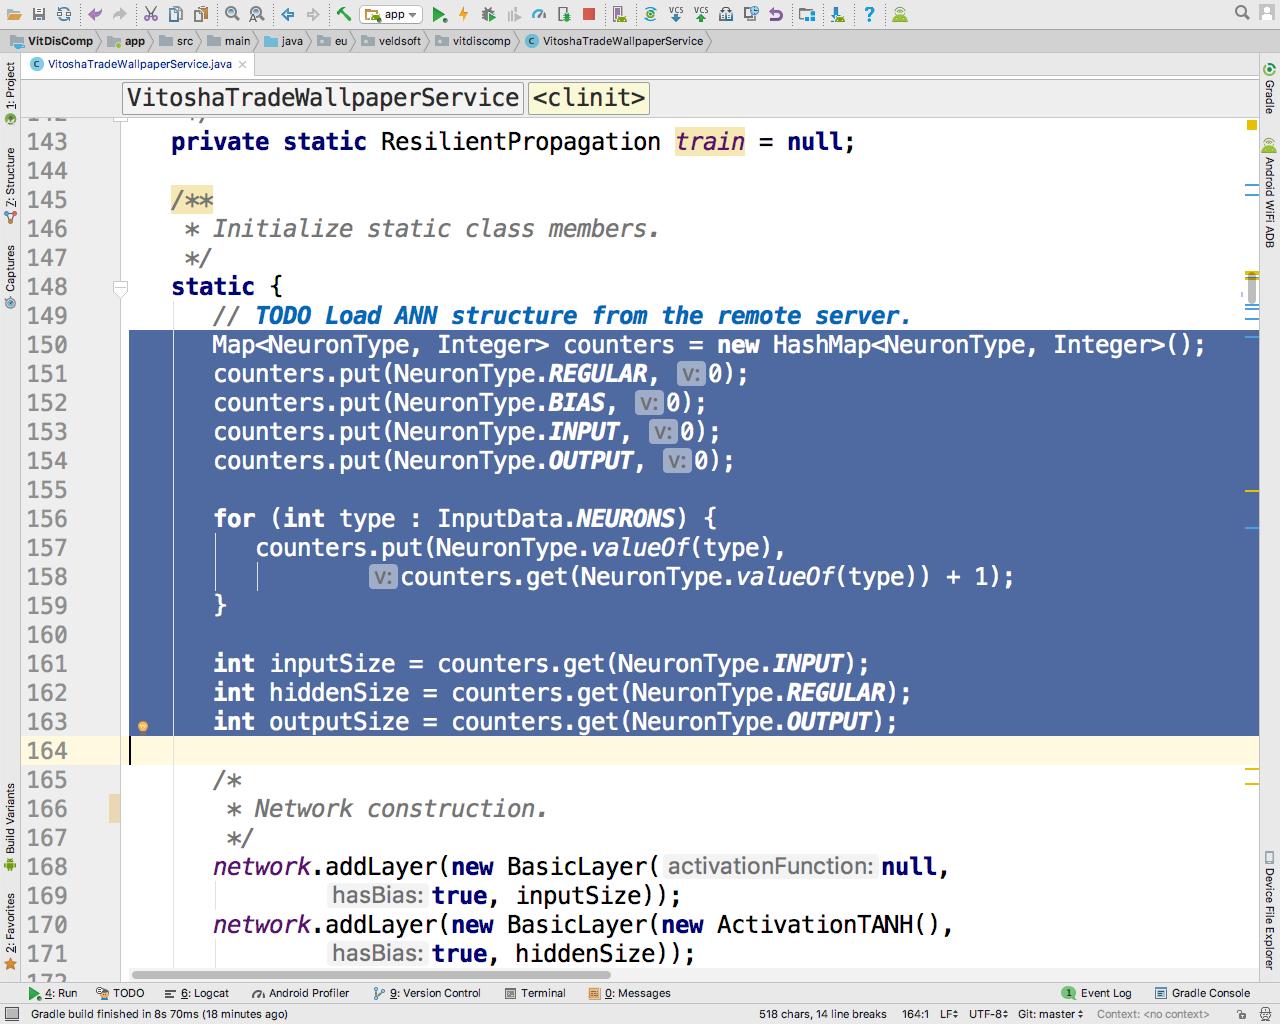
\includegraphics[height=0.45\pdfpageheight]{pic0036}
  \caption{Определяне на броя и типовете неврони}
\label{fig:pic0036}
\end{figure}
\FloatBarrier

Чрез сортиране с броене, ефективно се определя броят на невроните и техните типове (Фиг. \ref{fig:pic0036}).

\begin{figure}[h]
  \centering
  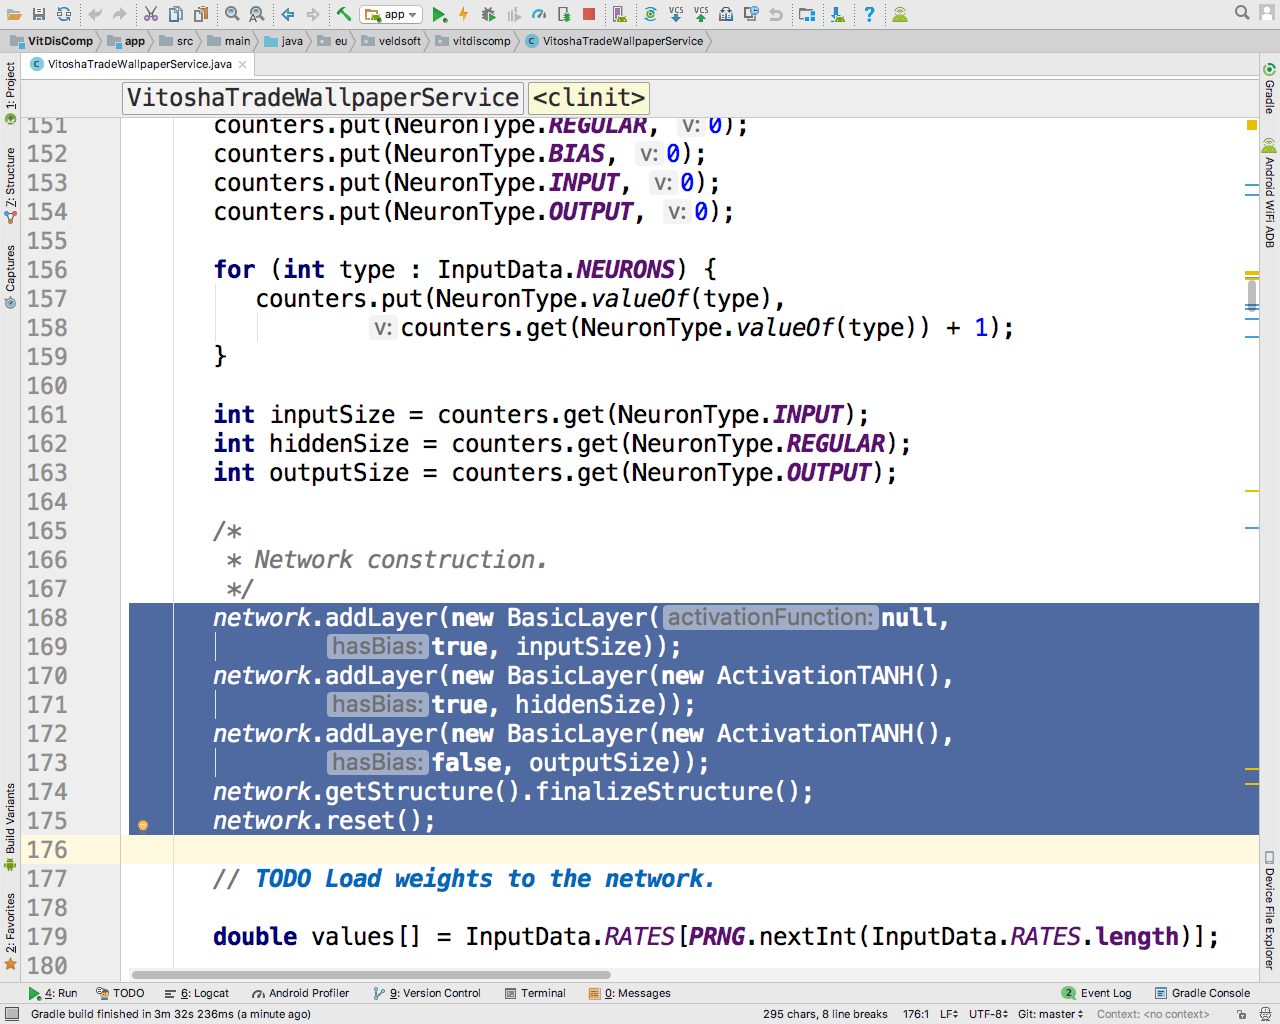
\includegraphics[height=0.45\pdfpageheight]{pic0037}
  \caption{Структура на трислойна изкуствена невронна мрежа}
\label{fig:pic0037}
\end{figure}
\FloatBarrier

За да се илюстрират възможностите за прогнозиране на изкуствените невронни мрежи, е избрана една от най-популярните структури, а именно трислойна невронна мрежа, която се обучава с обратно разпространение на грешката (Фиг. \ref{fig:pic0037}). Входният слой има единствената задача да получи сигналите от външната среда и поради тази причина не се задава активационна функция. За скрития и изходния слой е избрана функцията хиперболичен тангенс, тъй като тя е асимптотично сходима в безкрайностите по абсцисата и в същото време е симетрична по същата тази ос. Входният и скритият слоеве имат отместващ неврон (bias), който не е нужен в изходния слои, тъй като отместващият неврон винаги емитира високото ниво на сигнализация.

\begin{figure}[h]
  \centering
  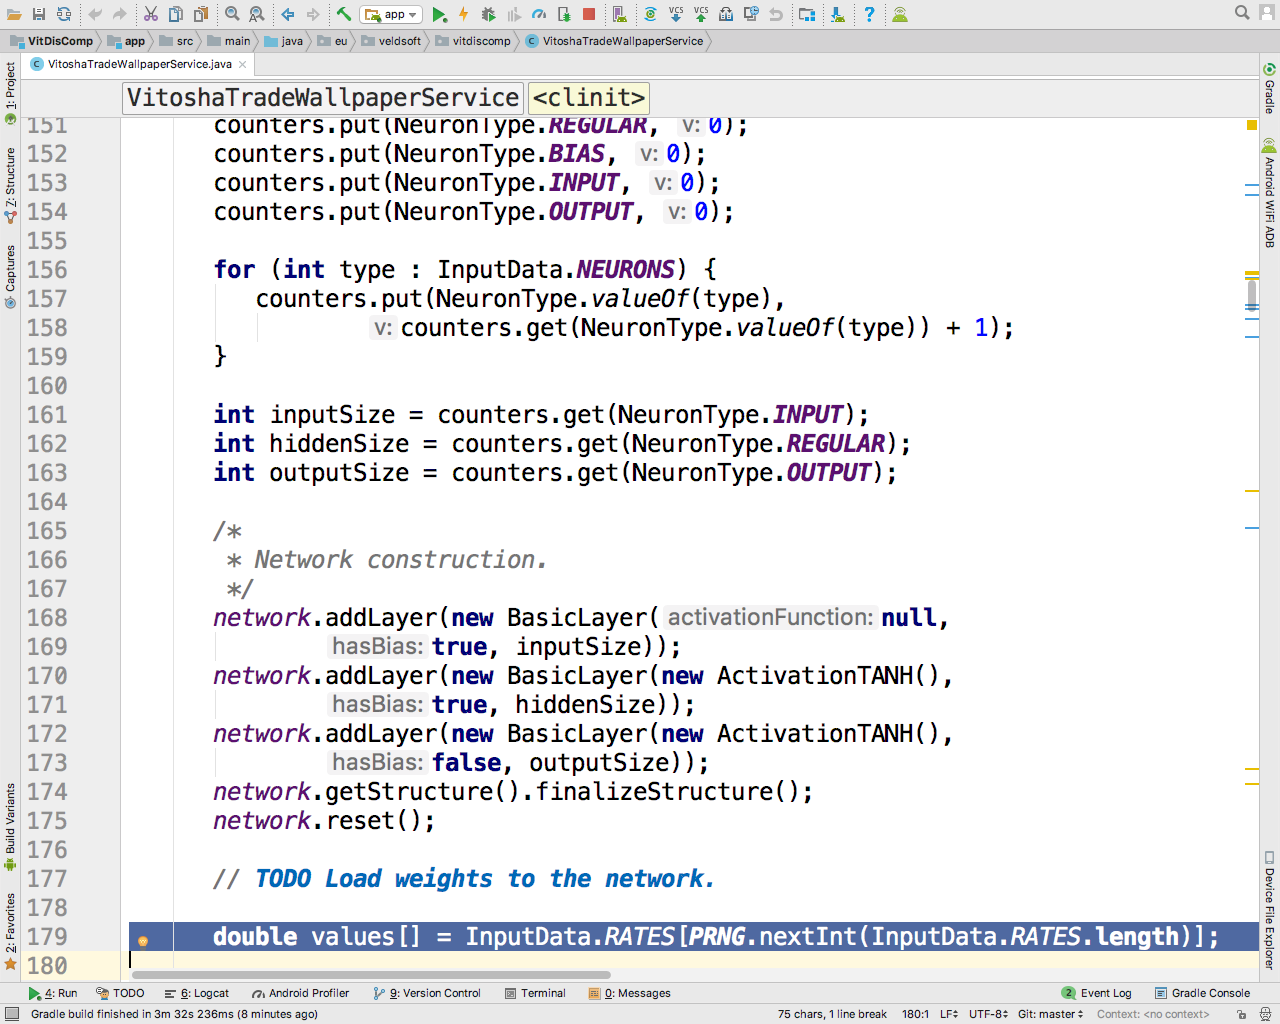
\includegraphics[height=0.45\pdfpageheight]{pic0038}
  \caption{Избор на стойности за прогнозиране}
\label{fig:pic0038}
\end{figure}
\FloatBarrier

От описанието на паралелните масиви при финансовите времеви редове ясно се вижда, че има четири възможни редици числа, които да се подават за прогнозиране към невронната мрежа (отваряне, най-ниско, най-високо, затваряне). 

\begin{figure}[h]
  \centering
  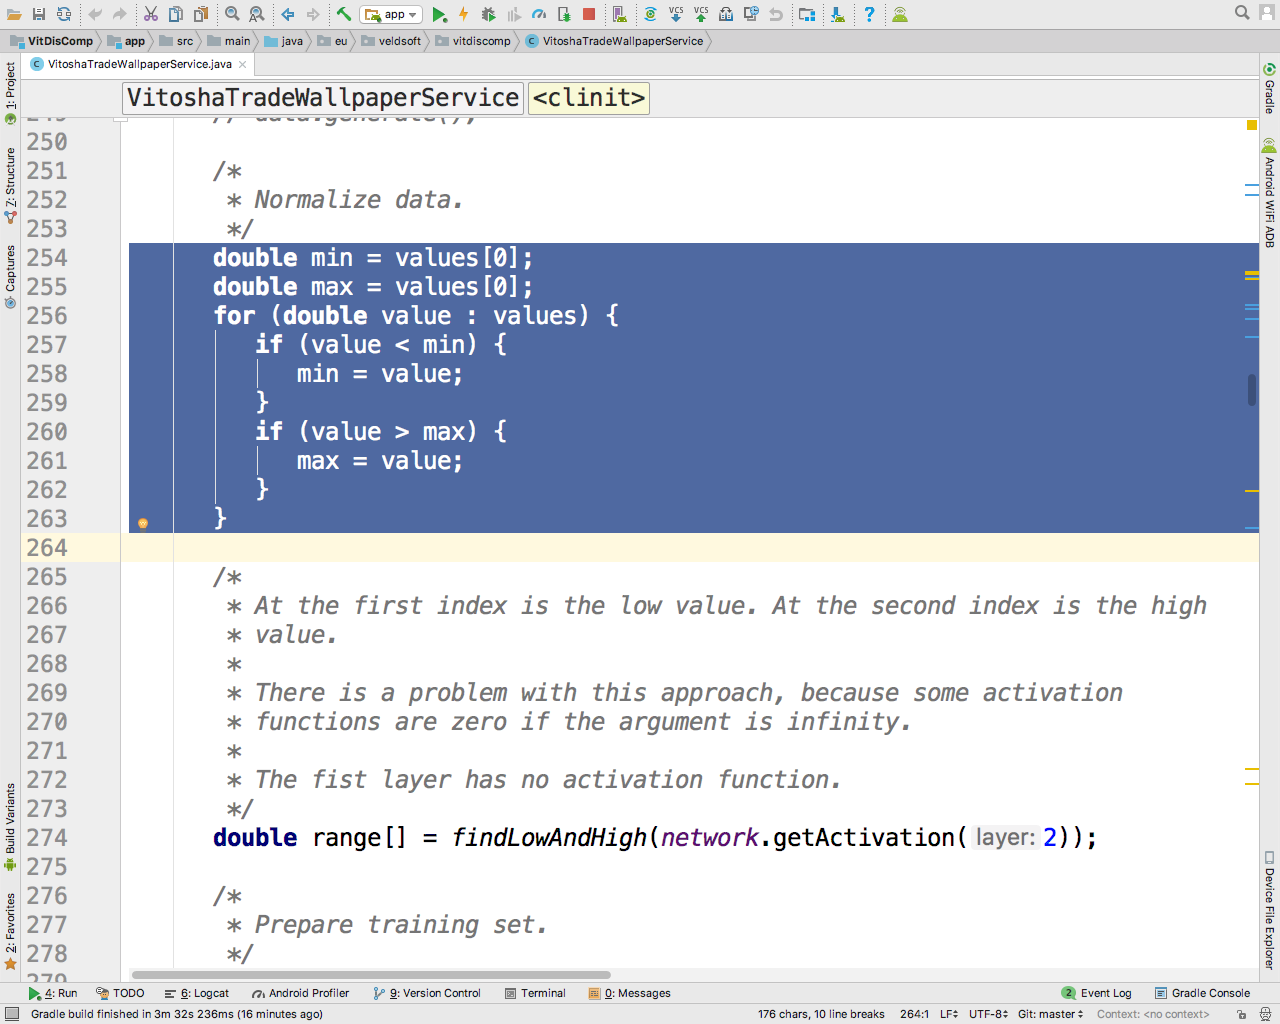
\includegraphics[height=0.45\pdfpageheight]{pic0039}
  \caption{Определяне на границите във времевия ред}
\label{fig:pic0039}
\end{figure}
\FloatBarrier

В практиката най-често се използва поредицата за стойности на затваряне, а целта е да се прогнозира нивото на отваряне в следващия времеви интервал. Целите на настоящото изложение не са реално постигане на финансови прогнози и поради тази причина на случаен принцип се избира коя последователност да бъде използвана при различните стартирания на обучението/прогнозирането (Фиг. \ref{fig:pic0038}).

\begin{figure}[h]
  \centering
  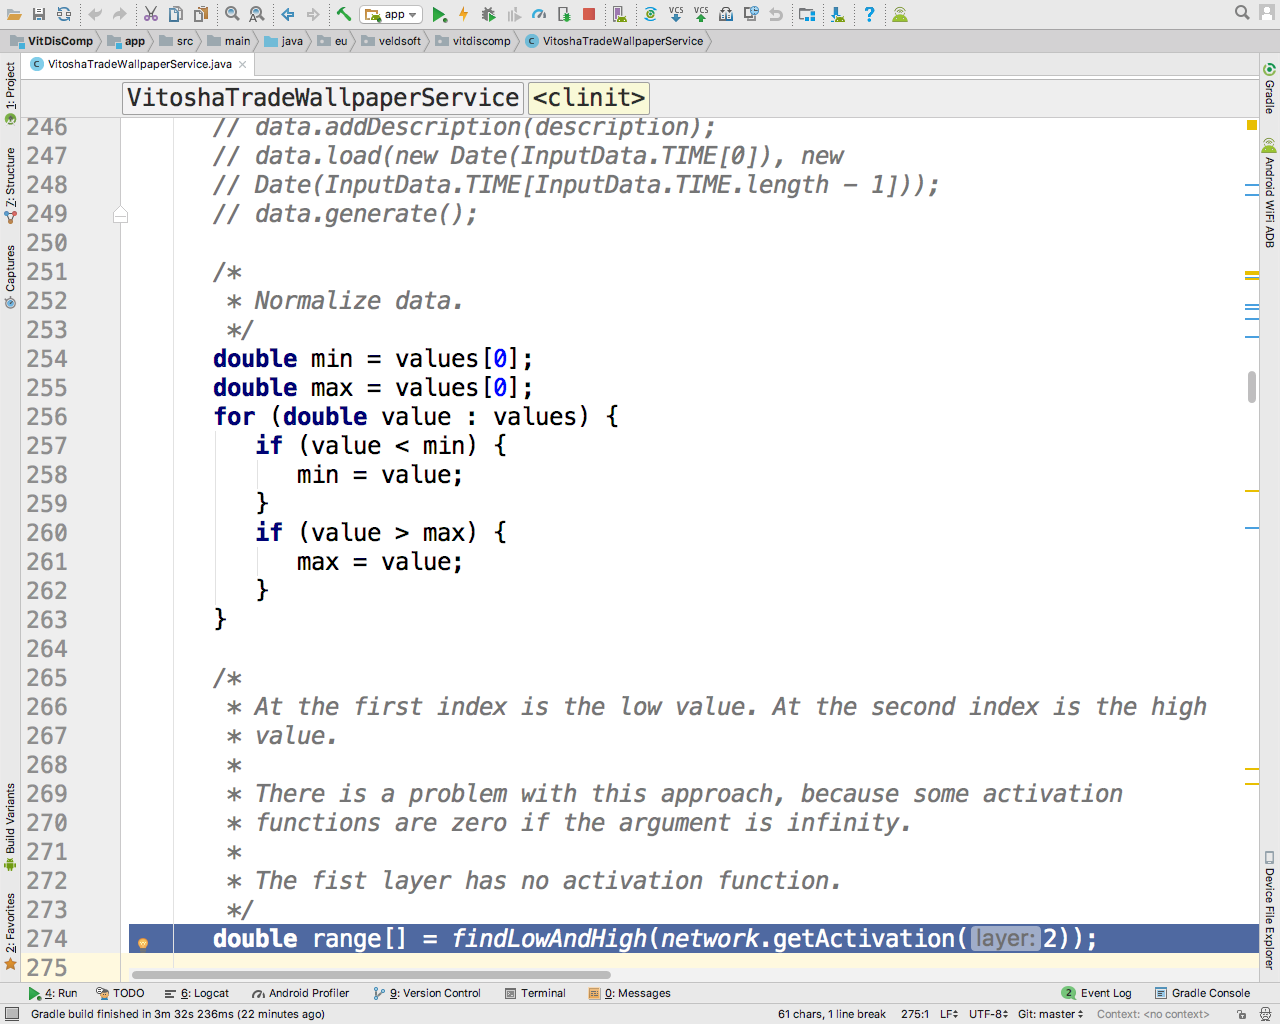
\includegraphics[height=0.45\pdfpageheight]{pic0040}
  \caption{Диапазон на активационната функция в изходния слой}
\label{fig:pic0040}
\end{figure}
\FloatBarrier

Тъй като целта е към системата за прогнозиране да се подават различни финансови времеви редове, то неизбежно се налага входната информация в системата да бъде предварително нормализирана, а първата стъпка към това е да се определят най-големата и най-малката стойности във времевия ред (Фиг. \ref{fig:pic0039}). В същото време данните трябва да бъдат съпоставени с диапазона, в който работят активационните функции на изкуствената невронна мрежа. В настоящото помагало е прието, че на входа ще се подадат сигнали в диапазона на функцията, използвана в изходния слой (Фиг. \ref{fig:pic0040}). Това решение се аргументира с факта, че информацията, подадена от невронната мрежа към външната среда, ще претърпи обратен процес на преоразмеряване, така че да има смисъл в конкретния финансов времеви ред.

\begin{figure}[h]
  \centering
  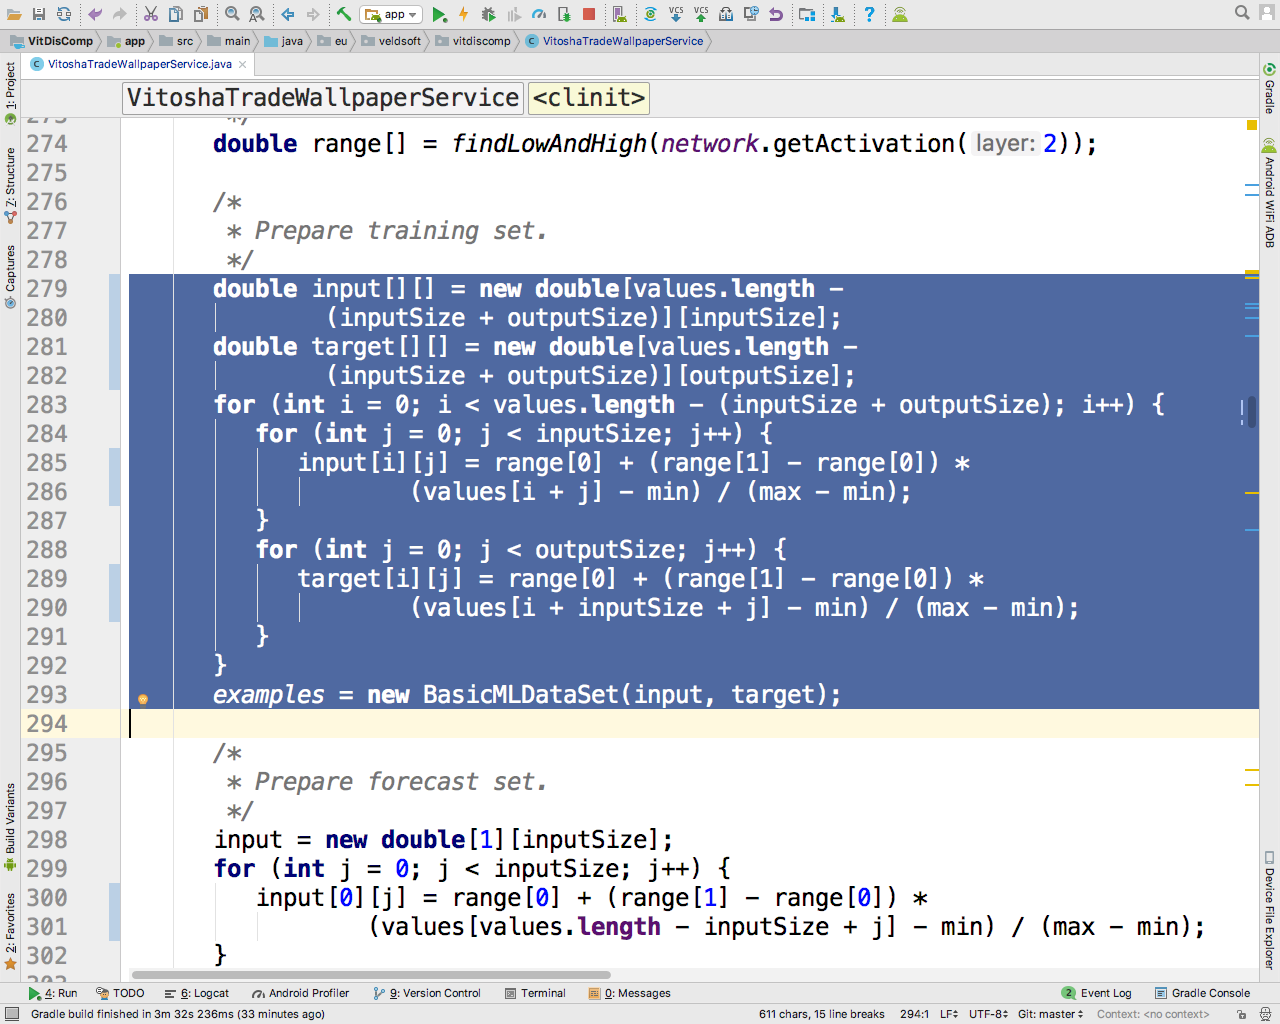
\includegraphics[height=0.45\pdfpageheight]{pic0041}
  \caption{Тренировъчни примери}
\label{fig:pic0041}
\end{figure}
\FloatBarrier

Нормализираните входни данни условно разделяме на две множества (измервания в миналото и измервания в бъдещето). Разделянето е условно, тъй като практически данните са от реални измервания в миналото (Фиг. \ref{fig:pic0041}).

\begin{figure}[h]
  \centering
  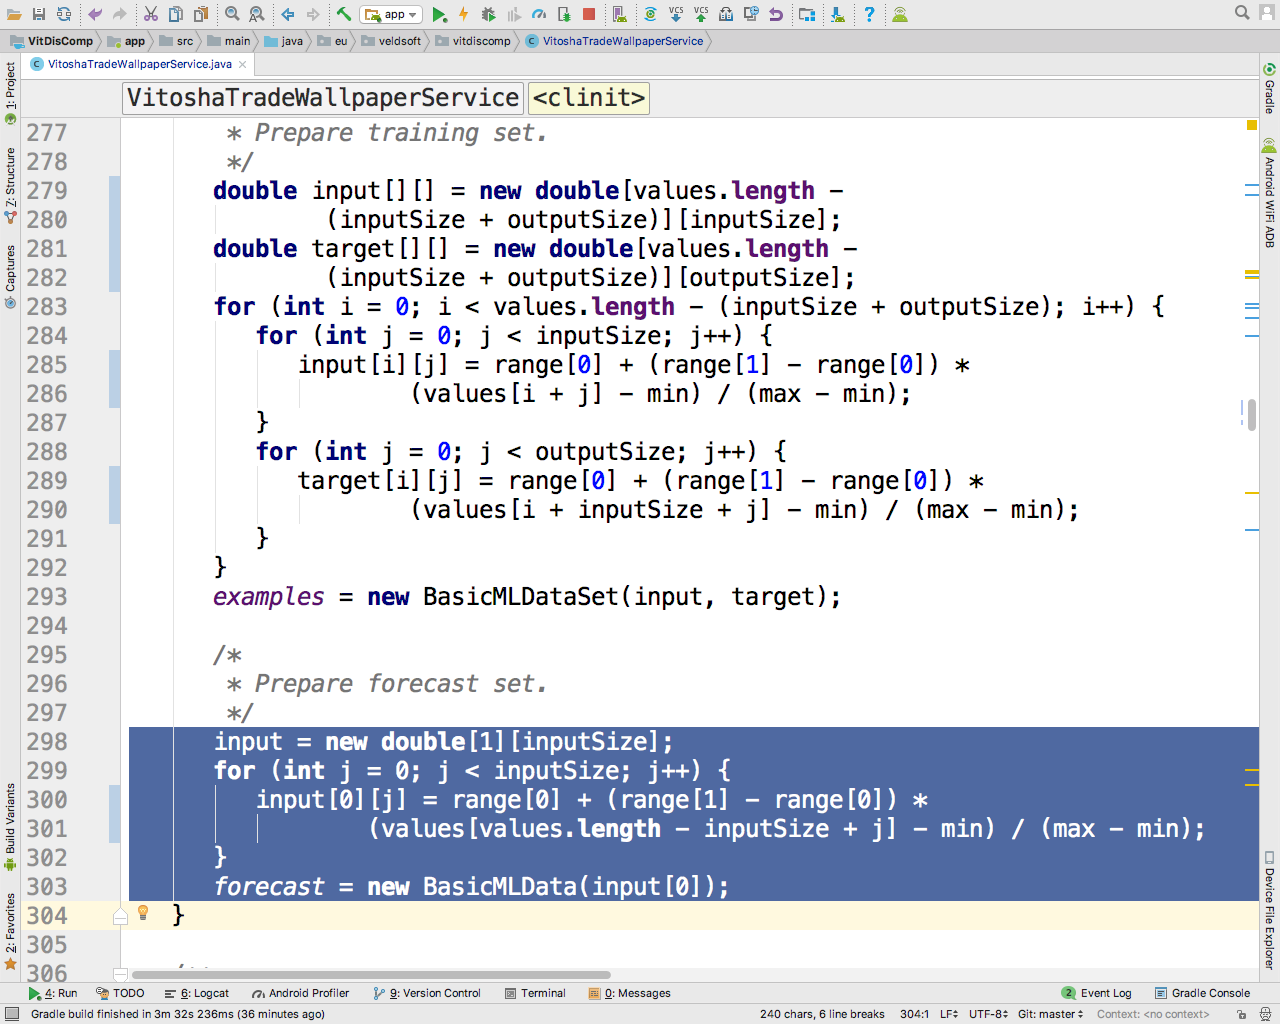
\includegraphics[height=0.45\pdfpageheight]{pic0042}
  \caption{Входни данни към изкуствената неверонна мрежа за получаване на прогноза}
\label{fig:pic0042}
\end{figure}
\FloatBarrier

Тъй като изкуствената невронна мрежа се използва и в двата й режима (обучение и прогнозиране), то се изготвя и вектор входни данни, спрямо които да бъде направена прогноза (Фиг. \ref{fig:pic0042}).

\begin{figure}[h]
  \centering
  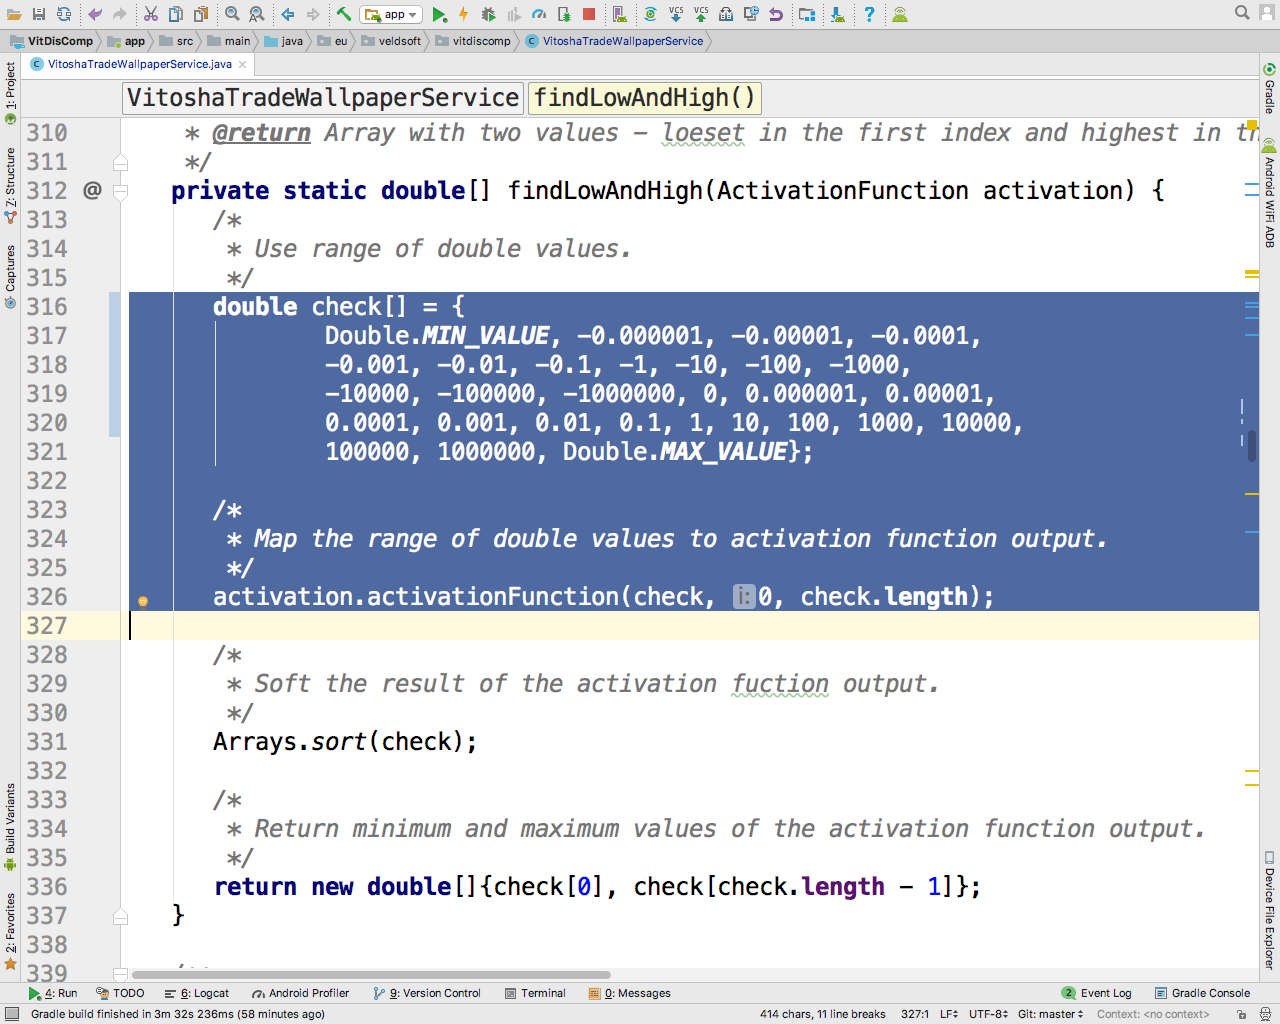
\includegraphics[height=0.45\pdfpageheight]{pic0043}
  \caption{Изследване на група от стойности за определяне на диапазона}
\label{fig:pic0043}
\end{figure}
\FloatBarrier

В общия случай активационните функции имат асимптотична сходимост и са монотонно нарастващи (Фиг. \ref{fig:pic0044}), което позволява техните крайни диапазони да бъдат установявани, чрез проверка на група от стойности (Фиг. \ref{fig:pic0043}).

\begin{figure}[h]
  \centering
  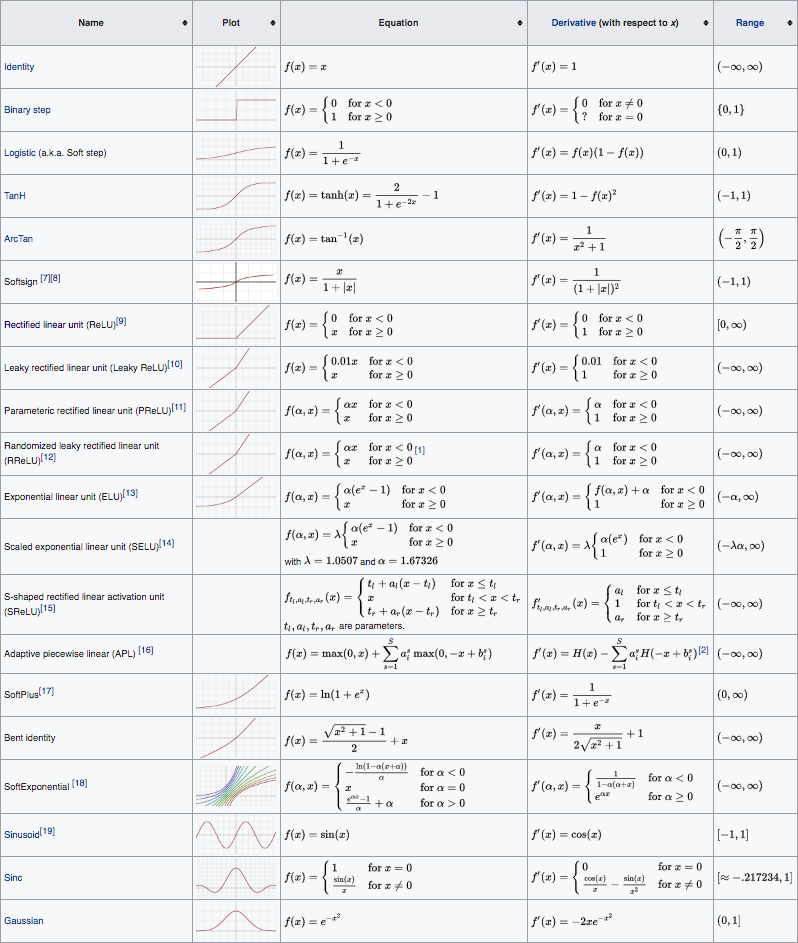
\includegraphics[height=0.7\pdfpageheight]{pic0044}
  \caption{Активационни функции \cite{afwiki}}
\label{fig:pic0044}
\end{figure}
\FloatBarrier

Както е добре видно на Фиг. \ref{fig:pic0044}, за някои от активационните функции такова определяне на диапазона може да се окаже силно подвеждащо (примерно при синус функцията). 

\begin{figure}[h]
  \centering
  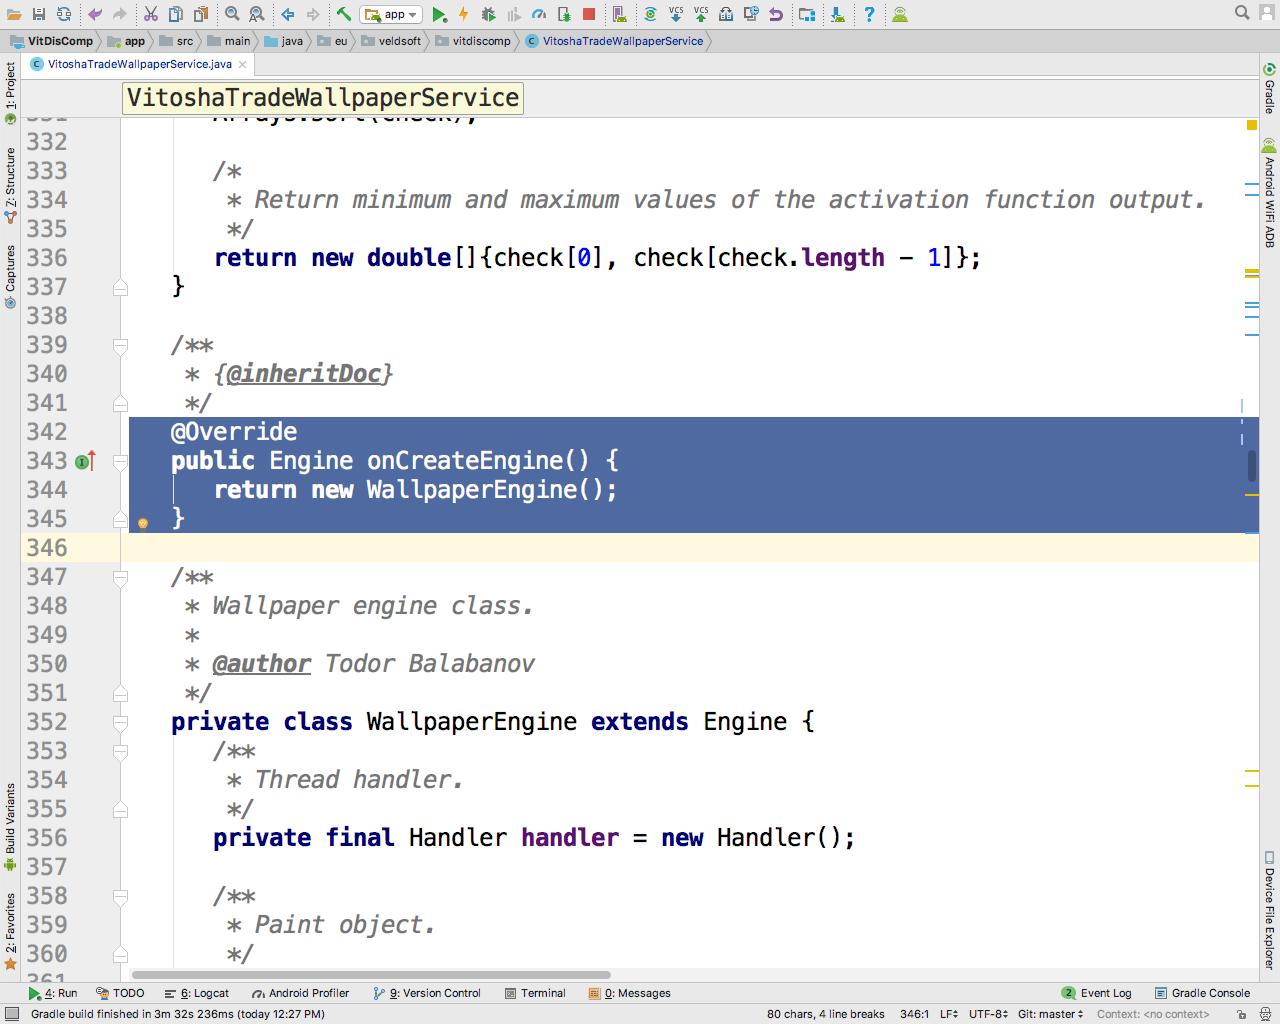
\includegraphics[height=0.45\pdfpageheight]{pic0045}
  \caption{Собствен engine обект}
\label{fig:pic0045}
\end{figure}
\FloatBarrier

Събитието за създаване на engine обект се предефинира, така че да се връща обект от нашия собствен клас за engine (Фиг. \ref{fig:pic0045}). 

\section{Двигател на услугата}

Същинската работа за фоново пресмятане в услугата се извършва от обект, описан с частен вътрешен клас от тип „двигател“ (Engine).

\begin{figure}[h]
  \centering
  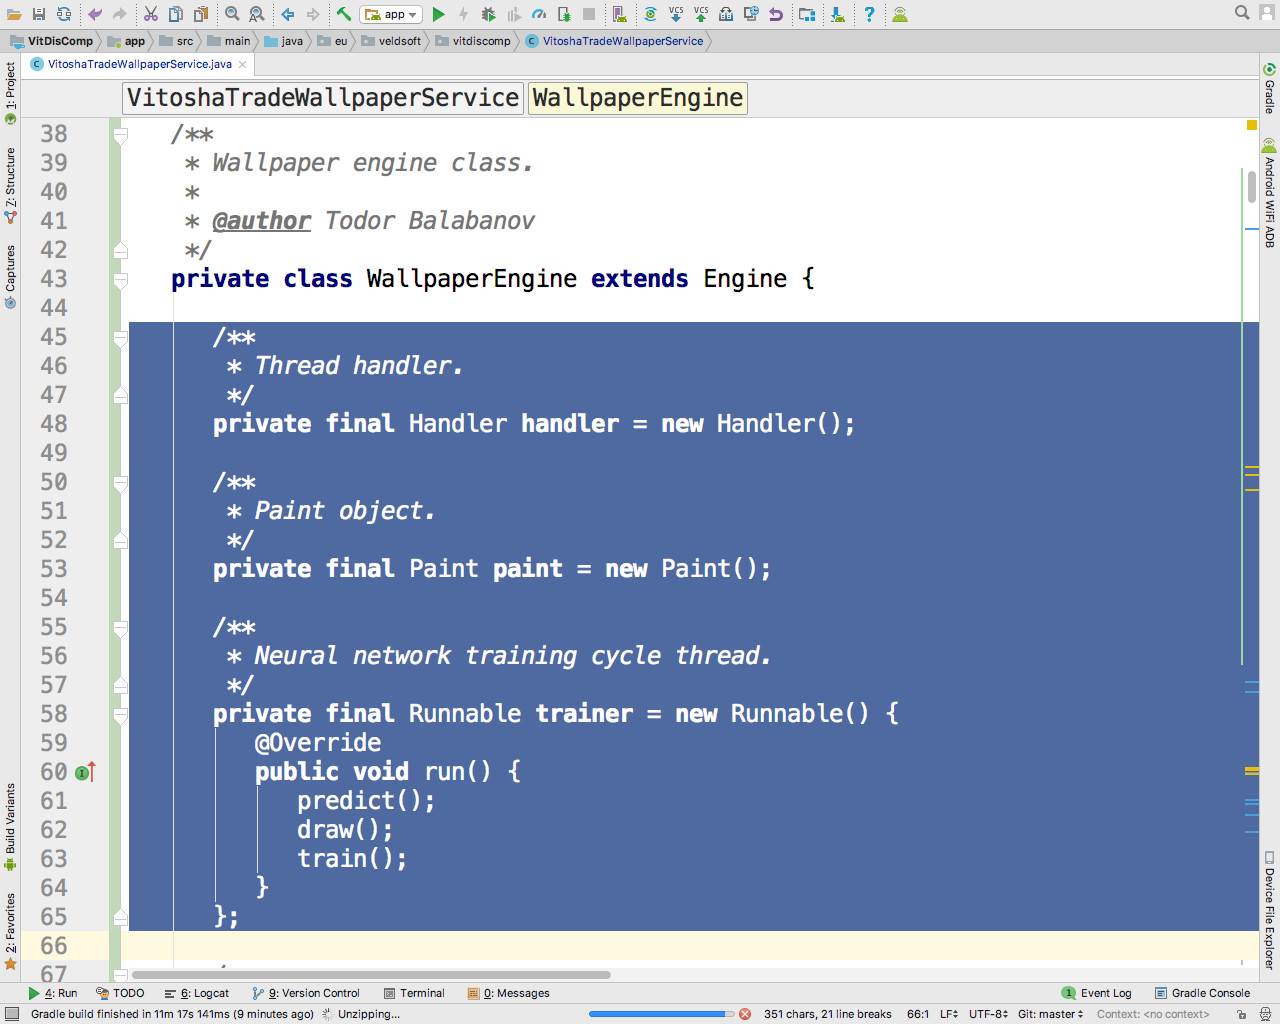
\includegraphics[height=0.45\pdfpageheight]{pic0046}
  \caption{Вътрешни променливи за двигателя на услугата}
\label{fig:pic0046}
\end{figure}
\FloatBarrier

В този двигател се използват три вътрешни променливи (Фиг. \ref{fig:pic0046}). Обектът от тип „четка“ (Paint) е само спомагателен и служи за еднократно определяне на характеристиките за изрисуване. Ползата е, че обектът бива създаден веднъж и след това се ползва през целия жизнен цикъл на услугата. 

\begin{figure}[h]
  \centering
  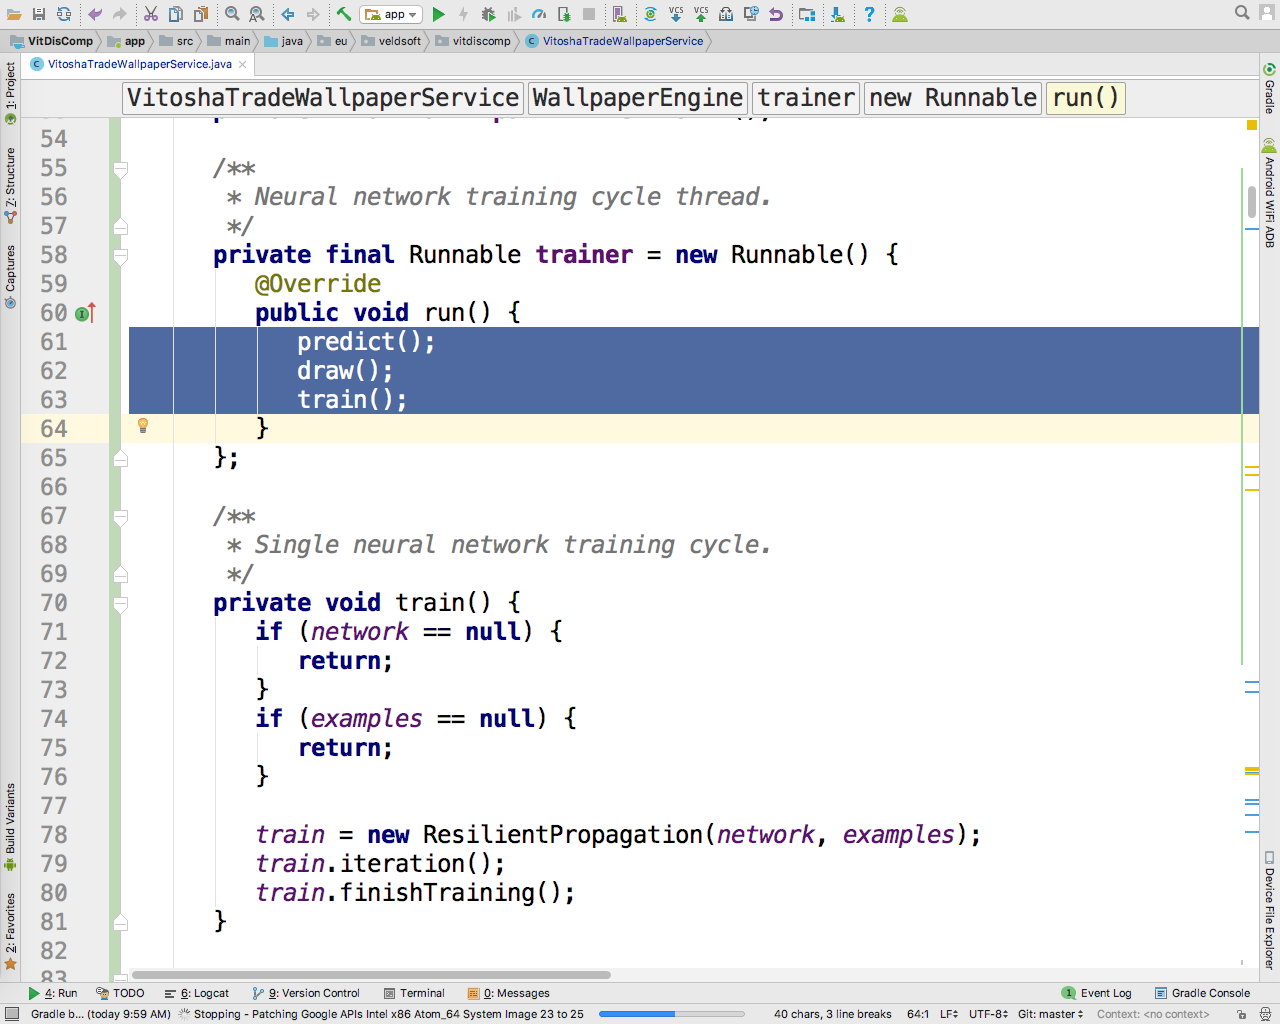
\includegraphics[height=0.45\pdfpageheight]{pic0047}
  \caption{Единичен цикъл във фонов режим}
\label{fig:pic0047}
\end{figure}
\FloatBarrier

За реалната работа на двигателя се дефинира отделна нишка (trainer), която да извършва операциите по генериране на прогноза, изчертаване на активния тапет и извършването на един цикъл от обучаващия процес на изкуствената невронна мрежа\index{изкуствени невронни мрежи} (Фиг. \ref{fig:pic0047}). Ефективното управление на нишки в Android се извършва с помощта на обекти „държател“ (Handler). Обектът държател поема отговорността по стартирането на нишката, спирането на нишката и реализацията на интервала за изчакване преди да бъде осъществено следващото събуждане на нишката. 

\begin{figure}[h]
  \centering
  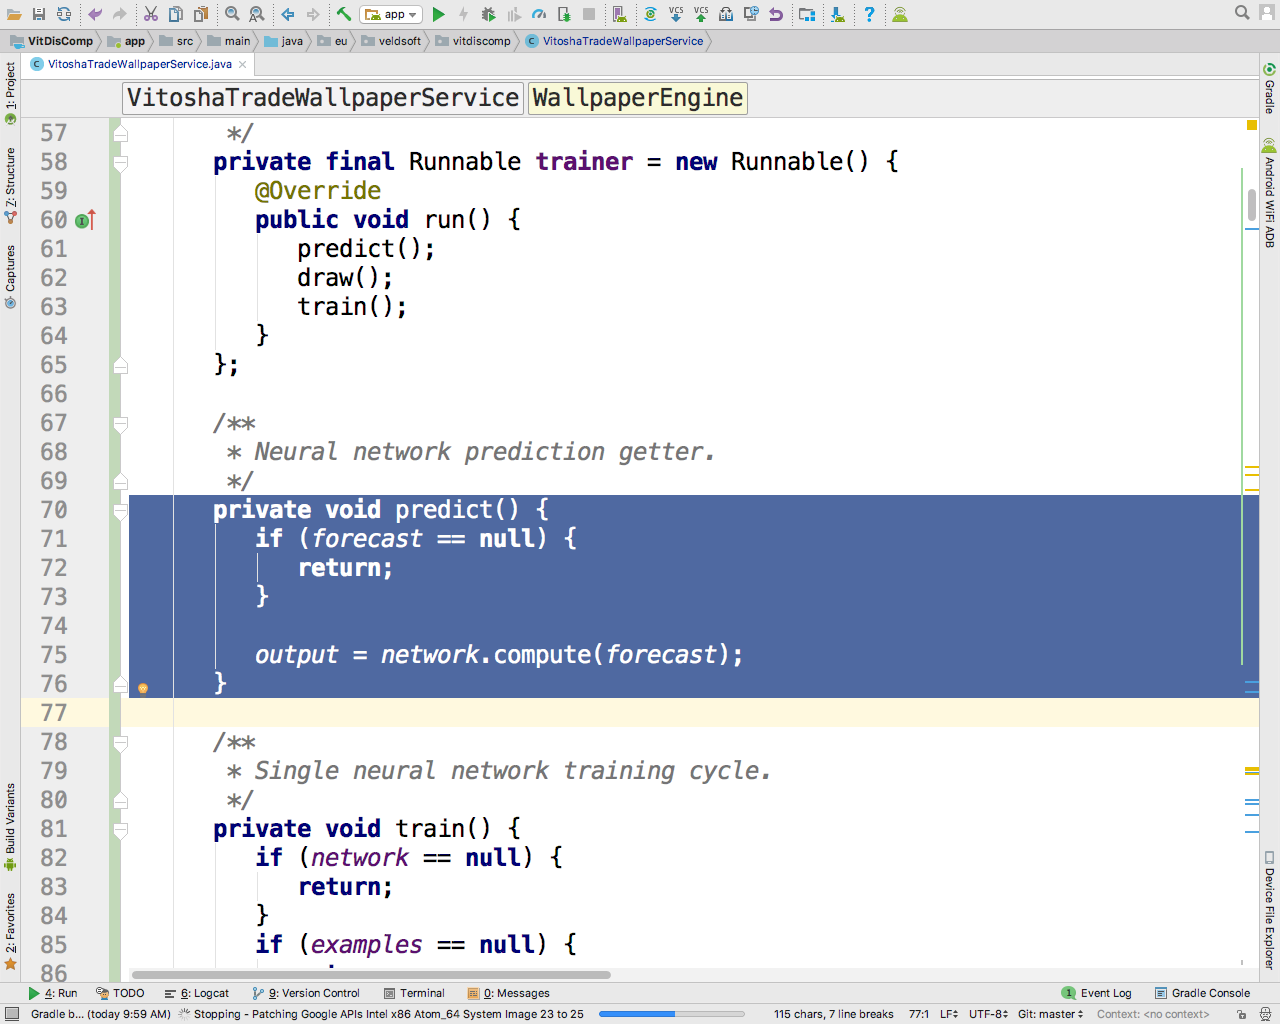
\includegraphics[height=0.45\pdfpageheight]{pic0048}
  \caption{Изчисляване на прогноза}
\label{fig:pic0048}
\end{figure}
\FloatBarrier

За да се изчисли прогноза, според текущото ниво на обученост на изкуствената невронна мрежа\index{изкуствени невронни мрежи}, е достатъчно мрежата да се активира в работен режим с подходящи данни към входния слой (Фиг. \ref{fig:pic0048}).

\begin{figure}[h]
  \centering
  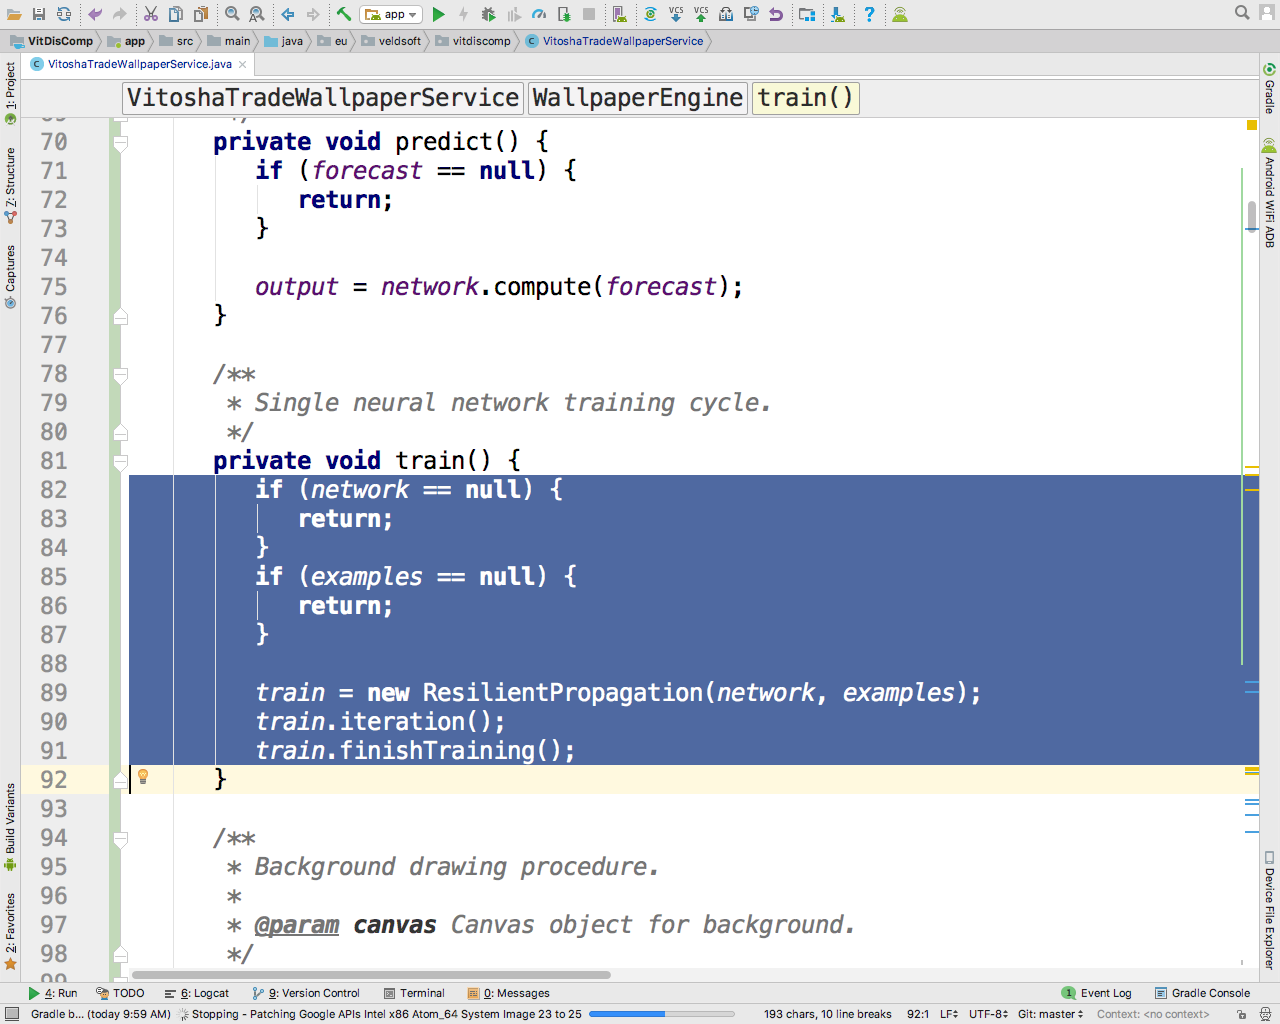
\includegraphics[height=0.45\pdfpageheight]{pic0049}
  \caption{Тренировъчен цикъл на изкуствената невронна мрежа}
\label{fig:pic0049}
\end{figure}
\FloatBarrier

За да се осъществи един тренировъчен цикъл на изкуствената невронна мрежа\index{изкуствени невронни мрежи}, е достатъчно да се създаде тренировъчен обект (в случая от еластично обратно разпространение на грешката\index{обратно разпространение на грешката}), към който се подават мрежата и тренировъчните примери (Фиг. \ref{fig:pic0049}).

\begin{figure}[h]
  \centering
  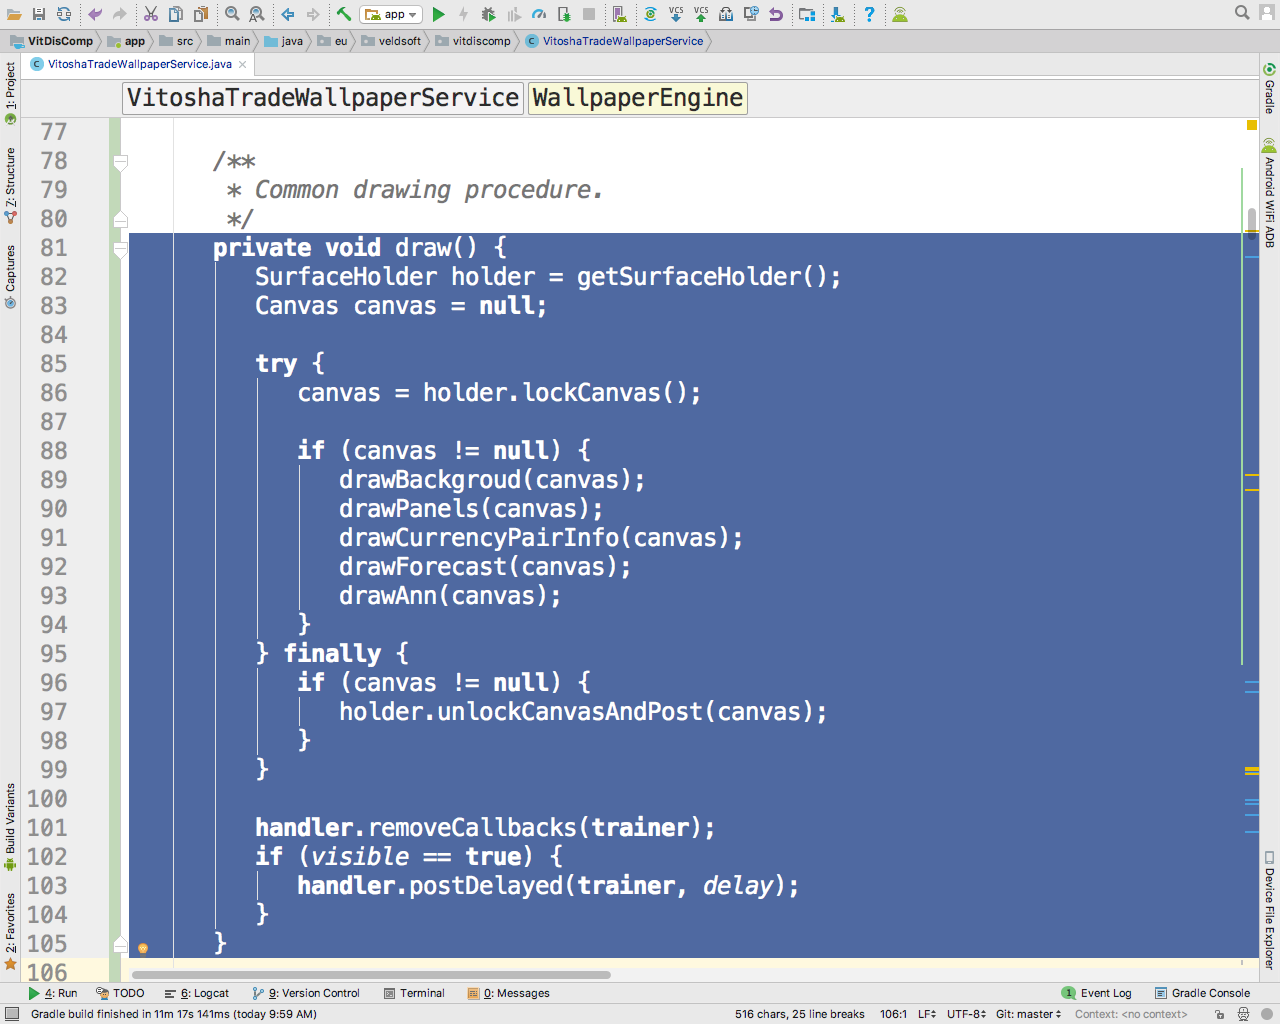
\includegraphics[height=0.45\pdfpageheight]{pic0050}
  \caption{Основна процедура по изрисуване на информацията от тренировъчния процес}
\label{fig:pic0050}
\end{figure}
\FloatBarrier

Изрисуването на информацията от тренировъчния процес е организирано в отделна функция (Фиг. \ref{fig:pic0050}). За да бъде осъществена визуалното представяне, се осигурява достъп до повърхността и платното, което тя съдържа. В самия край на функцията за визуално представяне се взема решение дали ще се изпълни следващ цикъл на обучение или изпълнението ще бъде преустановено. 

\begin{figure}[h]
  \centering
  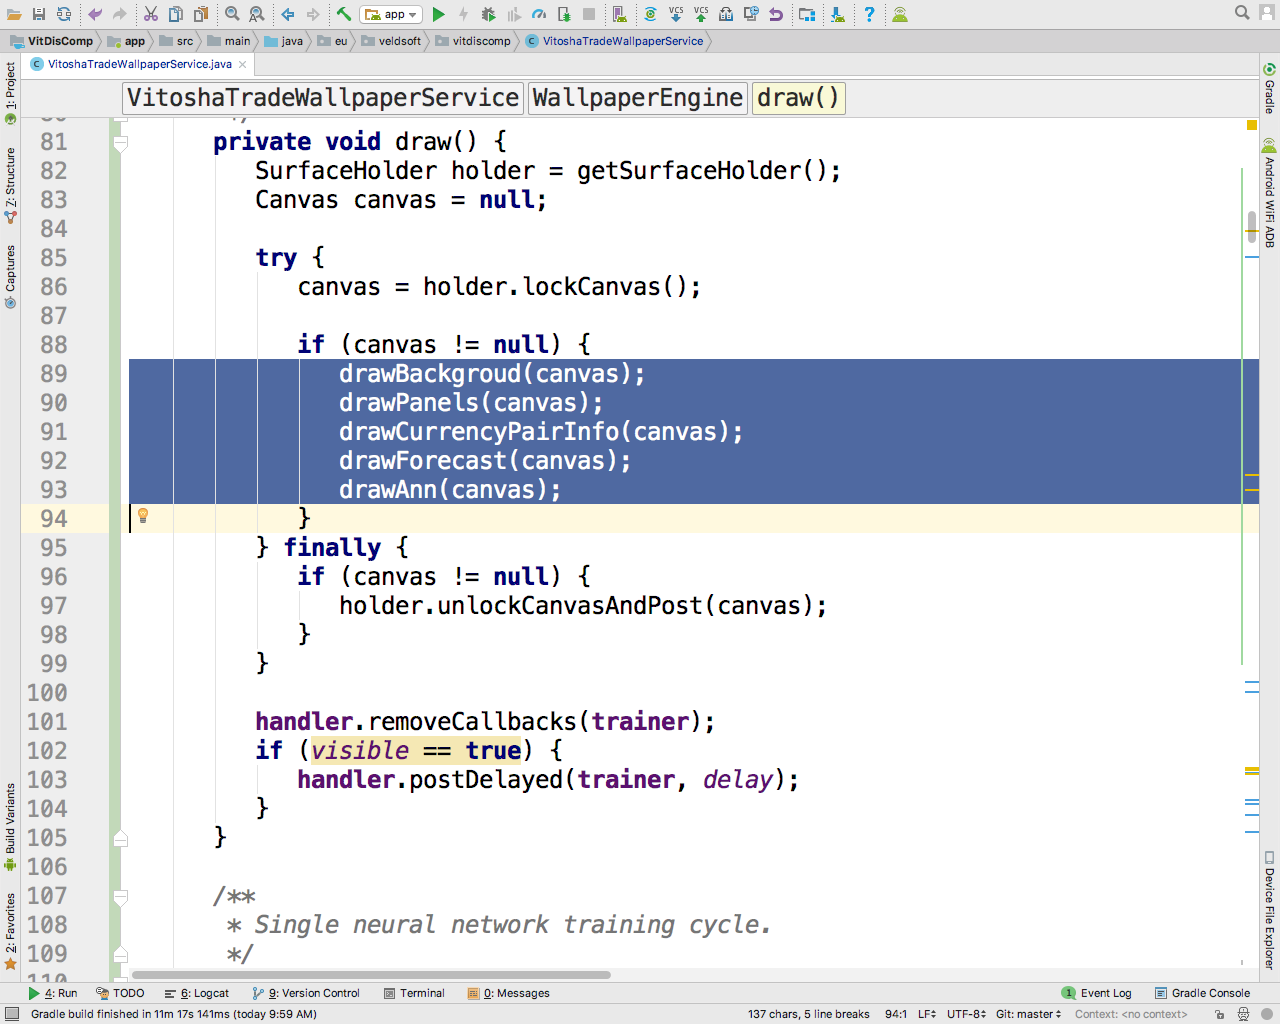
\includegraphics[height=0.45\pdfpageheight]{pic0051}
  \caption{Разбиване на задачата за визуално представяне}
\label{fig:pic0051}
\end{figure}
\FloatBarrier

Добрите практики за писане на програмен код включват разбиване на една сложна задача в група от множество по-прости задачи. Този принцип е приложен по отношение на визуалното представяне като са създадени пет помощни функции (Фиг. \ref{fig:pic0051}).  Първата функция изрисува фон, втората очертава полупрозрачни области за панелите, третата запълва панела с информация за валутната двойка, четвъртата показва информация в панела за текущо актуалната прогноза, а петата стилизиран модел на изкуствената невронна мрежа\index{изкуствени невронни мрежи}. 

\begin{figure}[h]
  \centering
  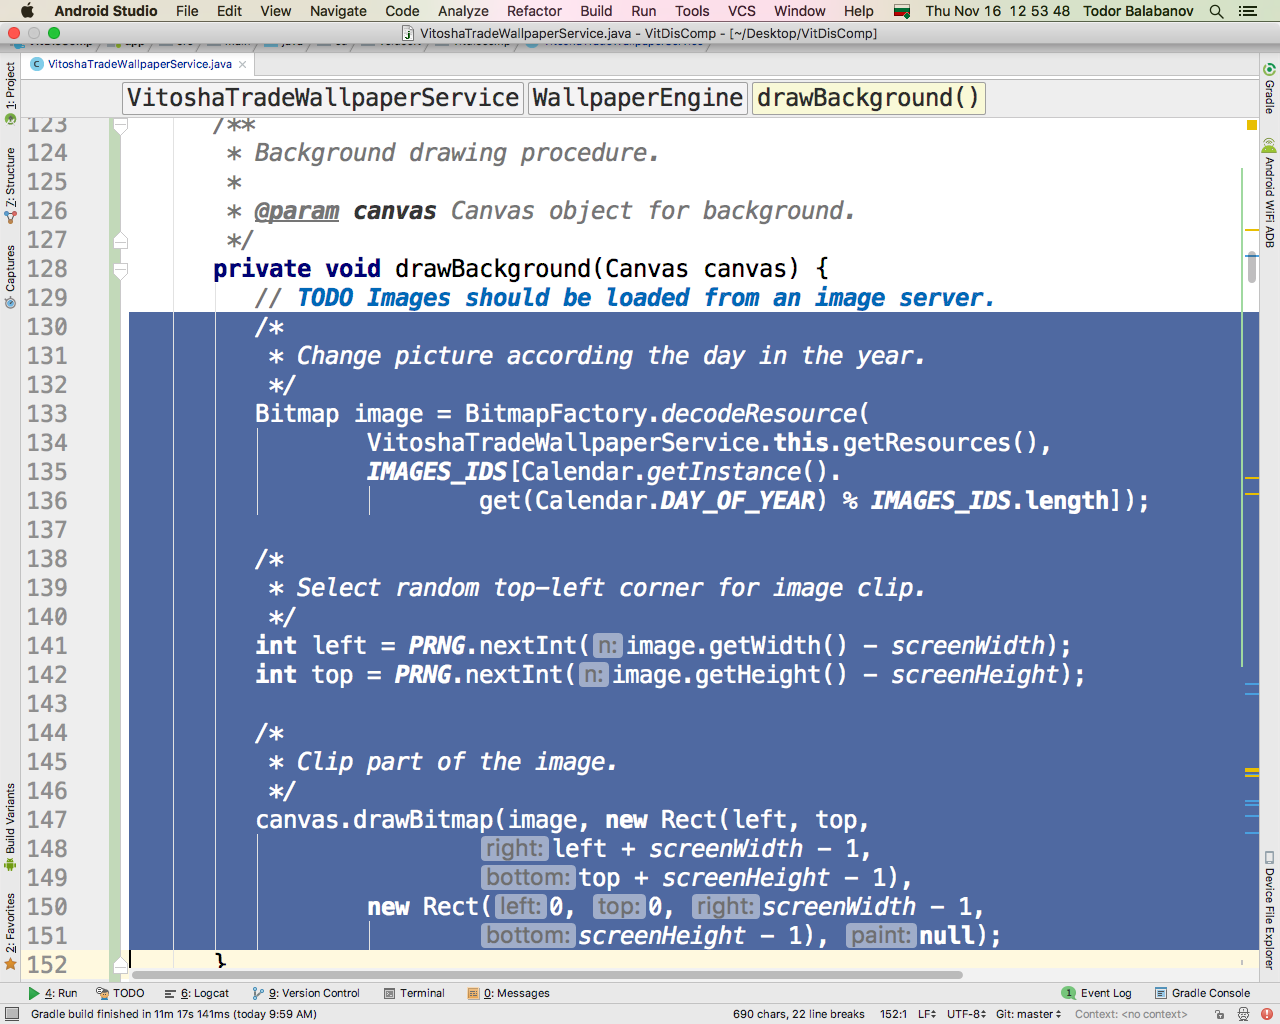
\includegraphics[height=0.45\pdfpageheight]{pic0052}
  \caption{Изрисуване на фона}
\label{fig:pic0052}
\end{figure}
\FloatBarrier

За да бъде изрисуван фонът, се зарежда предварително подготвено изображение и от него се отрязва такова парче, че да пасва на размерите на екрана (Фиг. \ref{fig:pic0052}). Коя част от изображението да бъде използвана се определя на случаен принцип.

\begin{figure}[h]
  \centering
  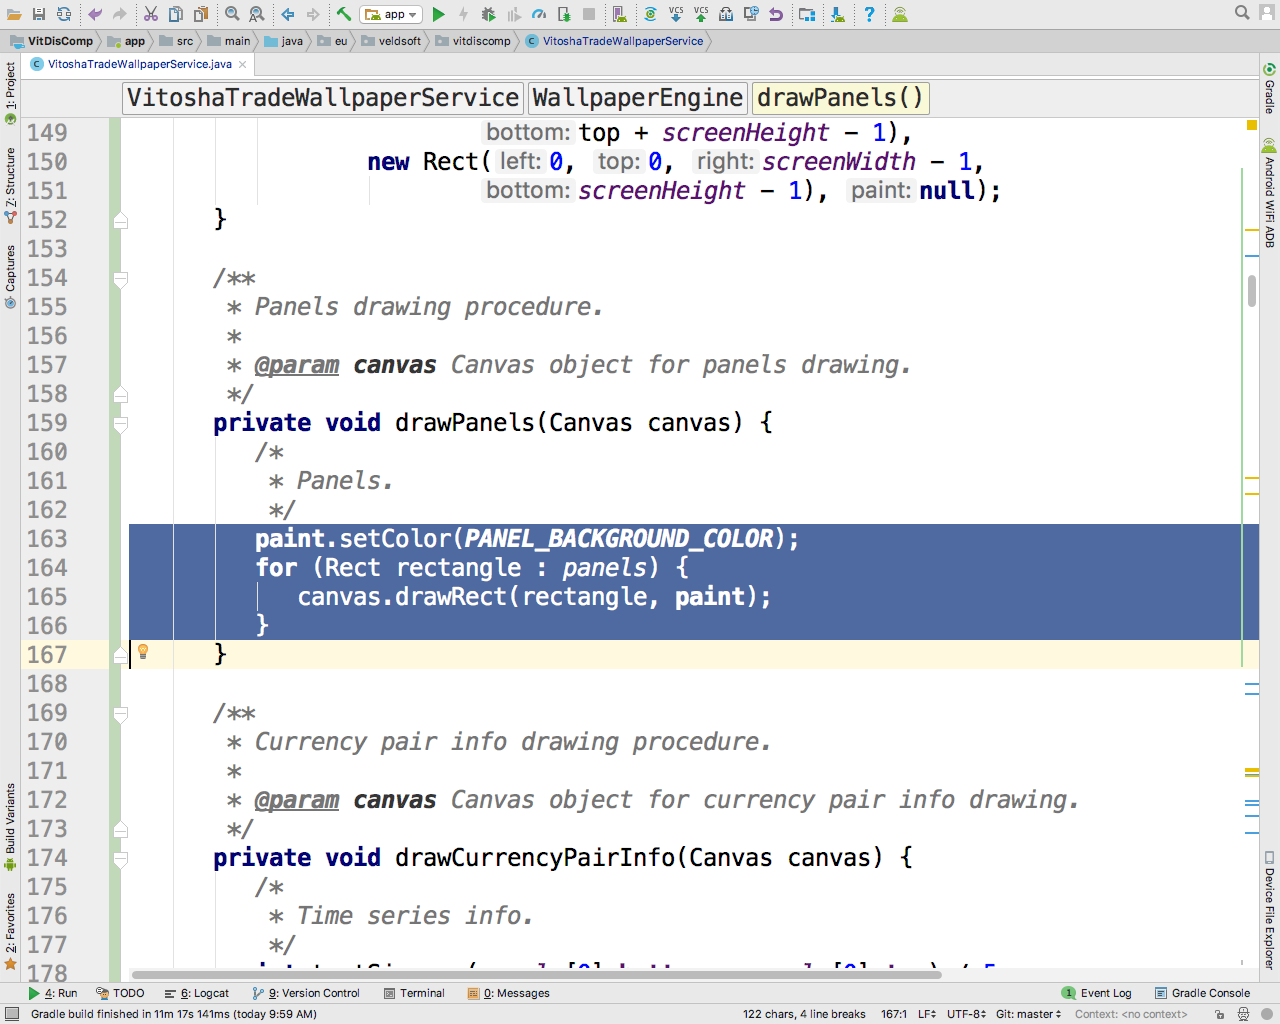
\includegraphics[height=0.45\pdfpageheight]{pic0053}
  \caption{Изрисуване на областите за служебна информация}
\label{fig:pic0053}
\end{figure}
\FloatBarrier

Веднага след изрисуването на фона се изрисуват и полупрозрачните петна за визуално представяне на информацията от процеса по обучението (Фиг. \ref{fig:pic0053}). Похватът за полупрозрачност е нужен, за да се избегне страничният ефект от сливане на цветове между служебната информация и фона. 

\begin{figure}[h]
  \centering
  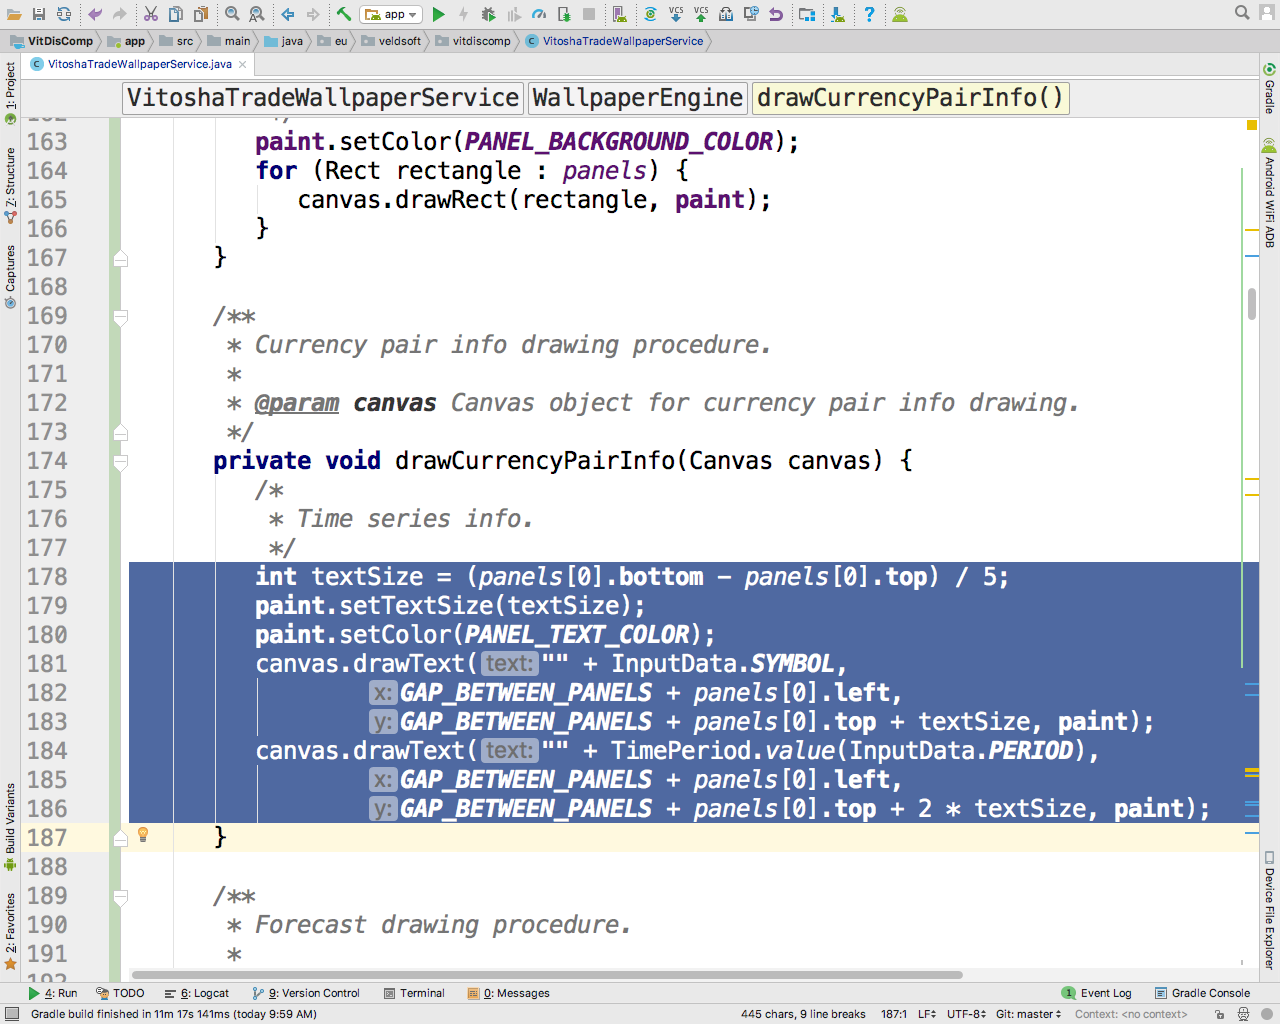
\includegraphics[height=0.45\pdfpageheight]{pic0054}
  \caption{Изрисуване на информацията за валутната двойка}
\label{fig:pic0054}
\end{figure}
\FloatBarrier

Информацията за валутната двойка се състои от название и времеви интервал на финансовия времеви ред (Фиг. \ref{fig:pic0054}). 

\begin{figure}[h]
  \centering
  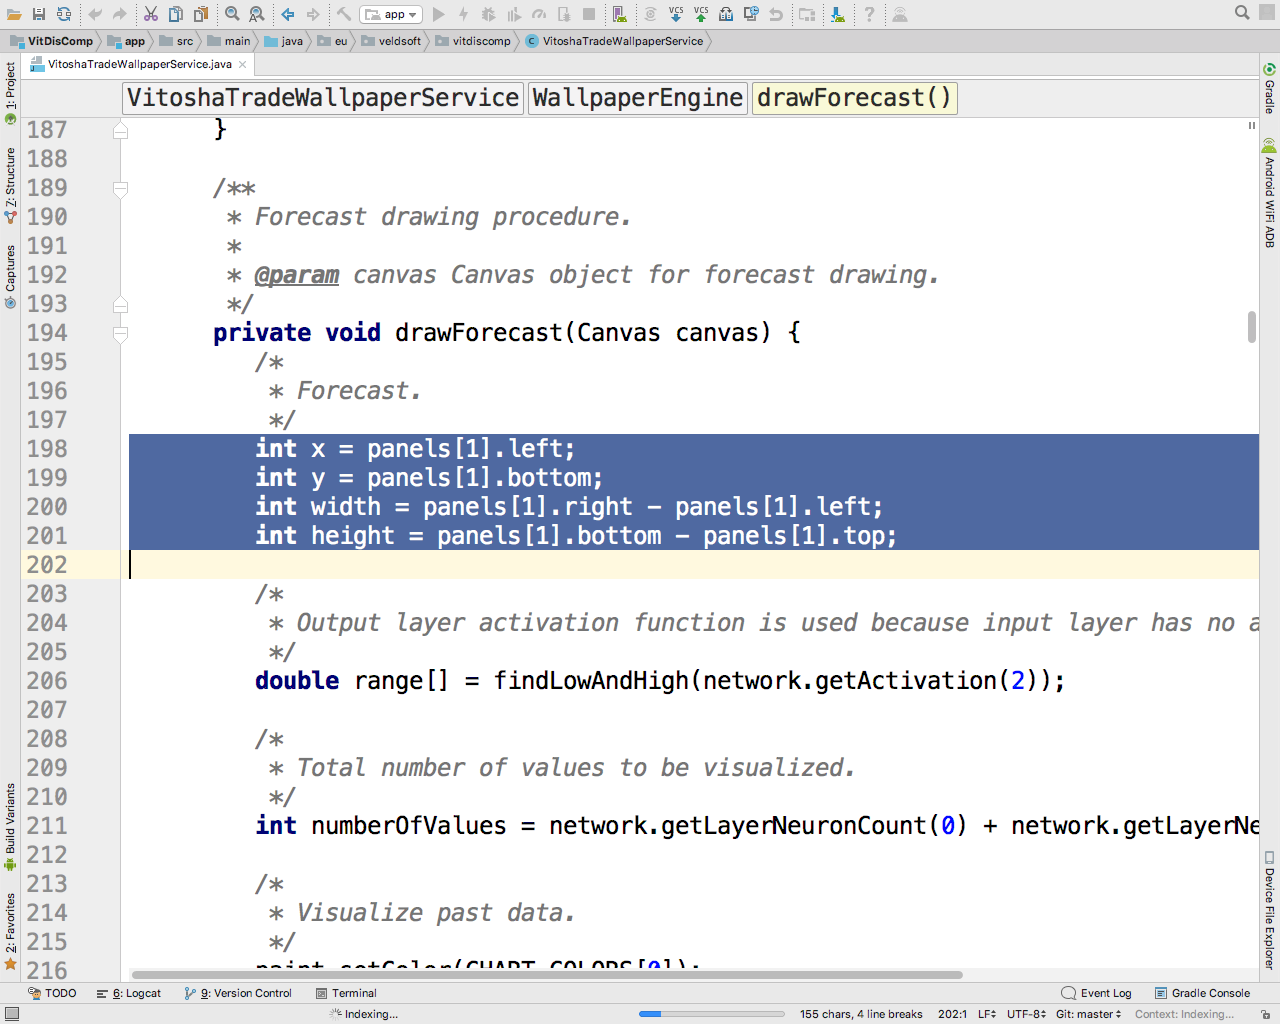
\includegraphics[height=0.45\pdfpageheight]{pic0055}
  \caption{Позиция и размери за визуално представяне на прогнозата}
\label{fig:pic0055}
\end{figure}
\FloatBarrier

Визуалното представяне на прогнозата изисква малко по-сложни пресмятания, така че информацията от входа и изхода да се поместят в рамките на определеното петно. За да бъде изпълнена тази задача, се вземат координатите и размерите на определената област (Фиг. \ref{fig:pic0055}). 

\begin{figure}[h]
  \centering
  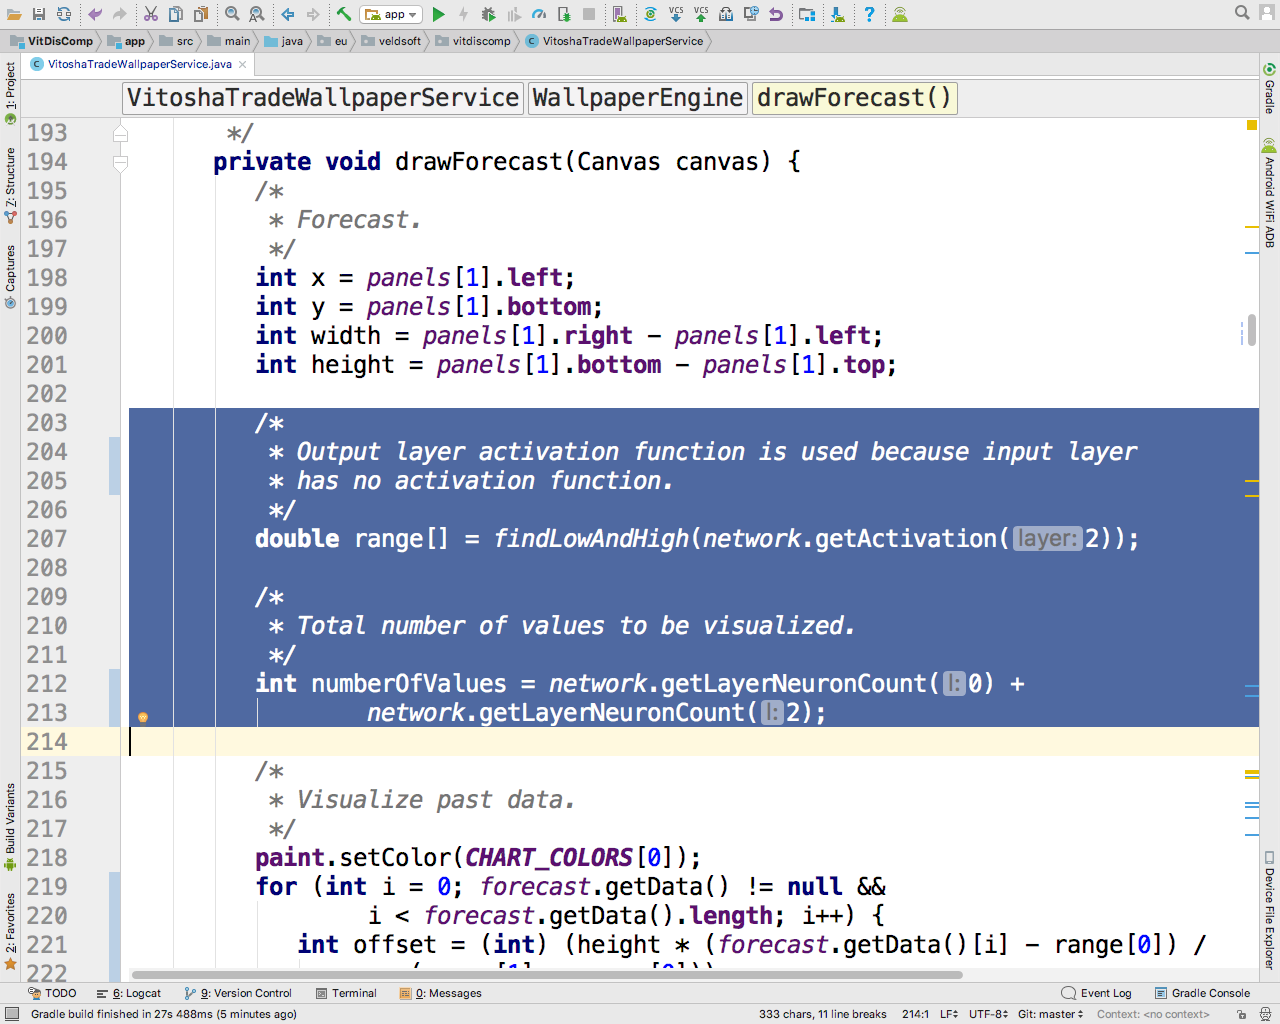
\includegraphics[height=0.45\pdfpageheight]{pic0056}
  \caption{Обхват на данните по ширина и височина}
\label{fig:pic0056}
\end{figure}
\FloatBarrier

За да бъдат визуализирани данните, е от съществено значение да се определи минималната и максималната стойности за вход-изхода, както и броят стойности, които ще бъдат визуализирани (Фиг. \ref{fig:pic0056}). В случая броят стойности за визуално представяне съвпада със сумата от броя входни въздействия и броя изходни сигнали. 

\begin{figure}[h]
  \centering
  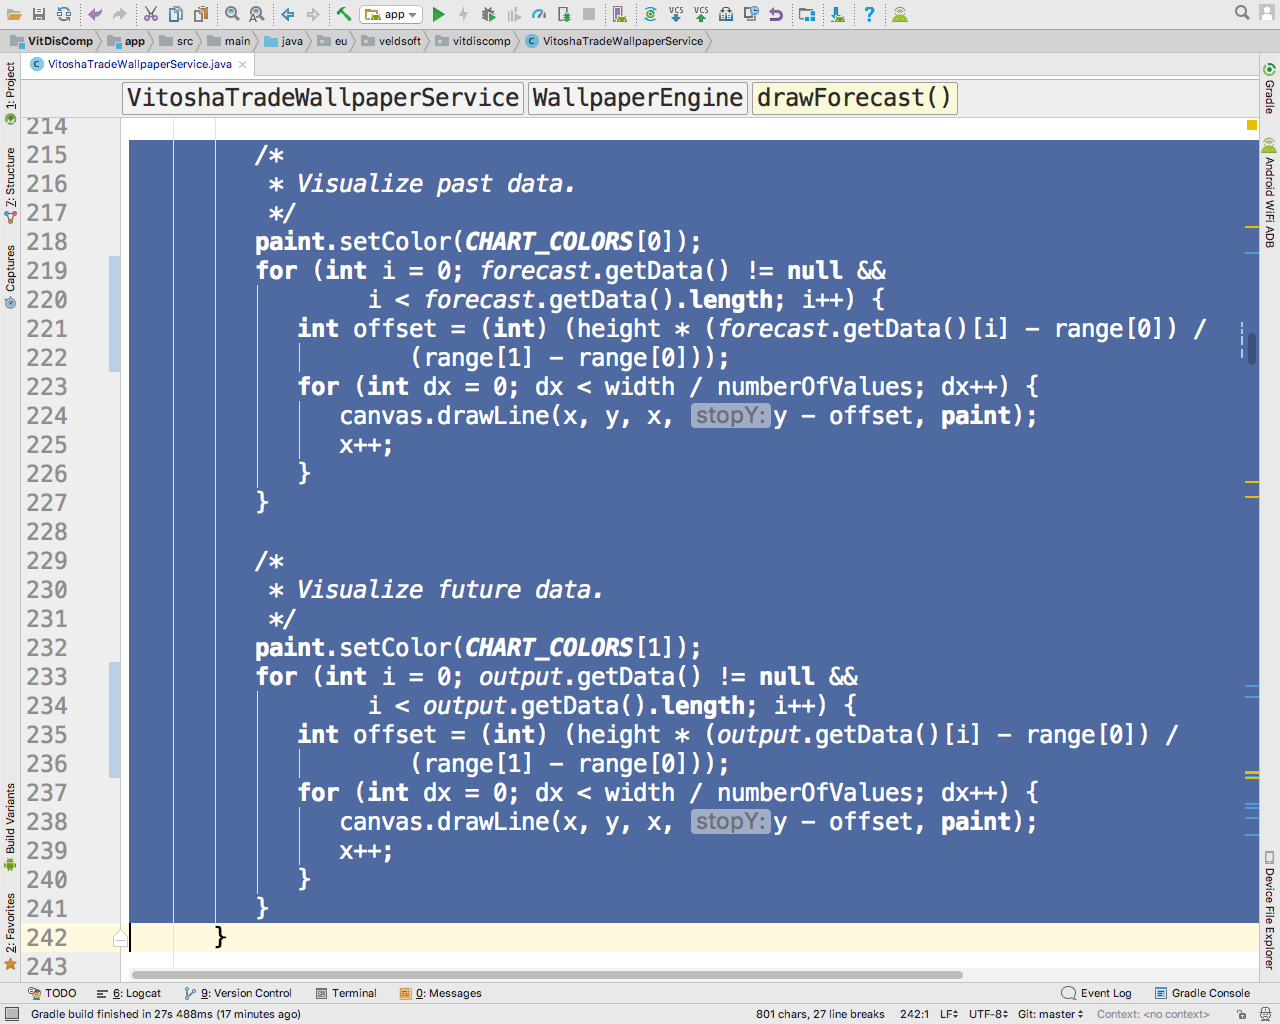
\includegraphics[height=0.45\pdfpageheight]{pic0057}
  \caption{Цикли за визуално представяне на стълбовете от времевия реди и прогнозата}
\label{fig:pic0057}
\end{figure}
\FloatBarrier

Данните за отминалия период от време се показват с един цвят, а данните за прогнозата в друг цвят (Фиг. \ref{fig:pic0057}). Самата визуално представяне представлява стълбова диаграма (bar-chart) на входните данни и на прогнозата. 

\begin{figure}[h]
  \centering
  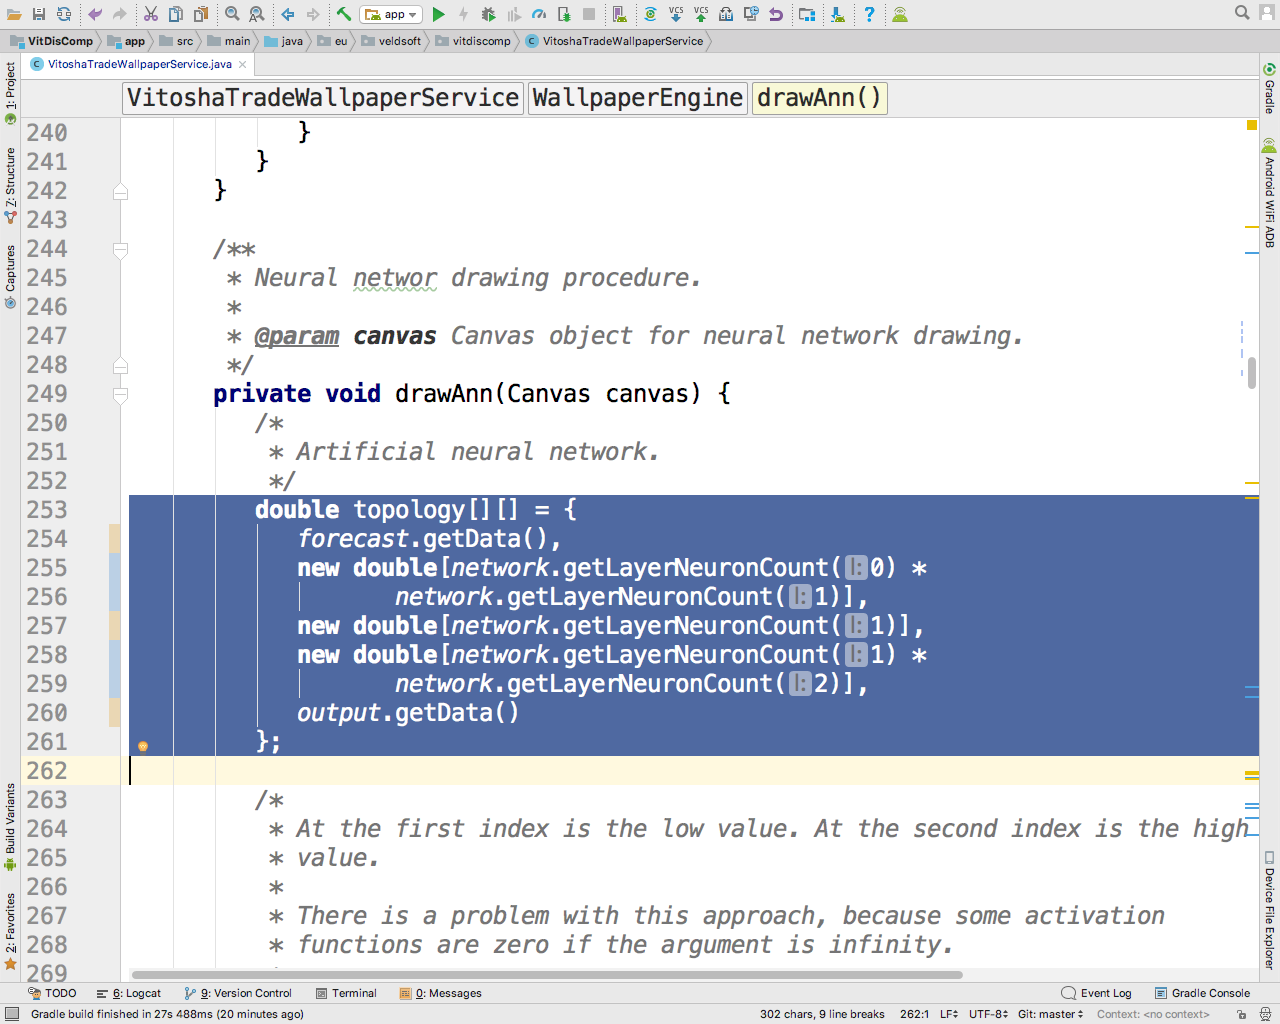
\includegraphics[height=0.45\pdfpageheight]{pic0058}
  \caption{Топология на изкуствената невронна мрежа, която се визуализира}
\label{fig:pic0058}
\end{figure}
\FloatBarrier

В третата област за визуално представяне се изрисува стилизирана информация за състоянието на изкуствената невронна мрежа\index{изкуствени невронни мрежи}. Областта е правоъгълна и бива разделена на пет вертикални зони: 1. Стойности на невроните във входния слой; 2. Стойности на теглата между входния и скрития слой; 3. Стойности на невроните в скрития слой; 4. Стойности на теглата между скрития и изходния слой; 5. Стойности на невроните в изходния слой (Фиг. \ref{fig:pic0058}).

\begin{figure}[h]
  \centering
  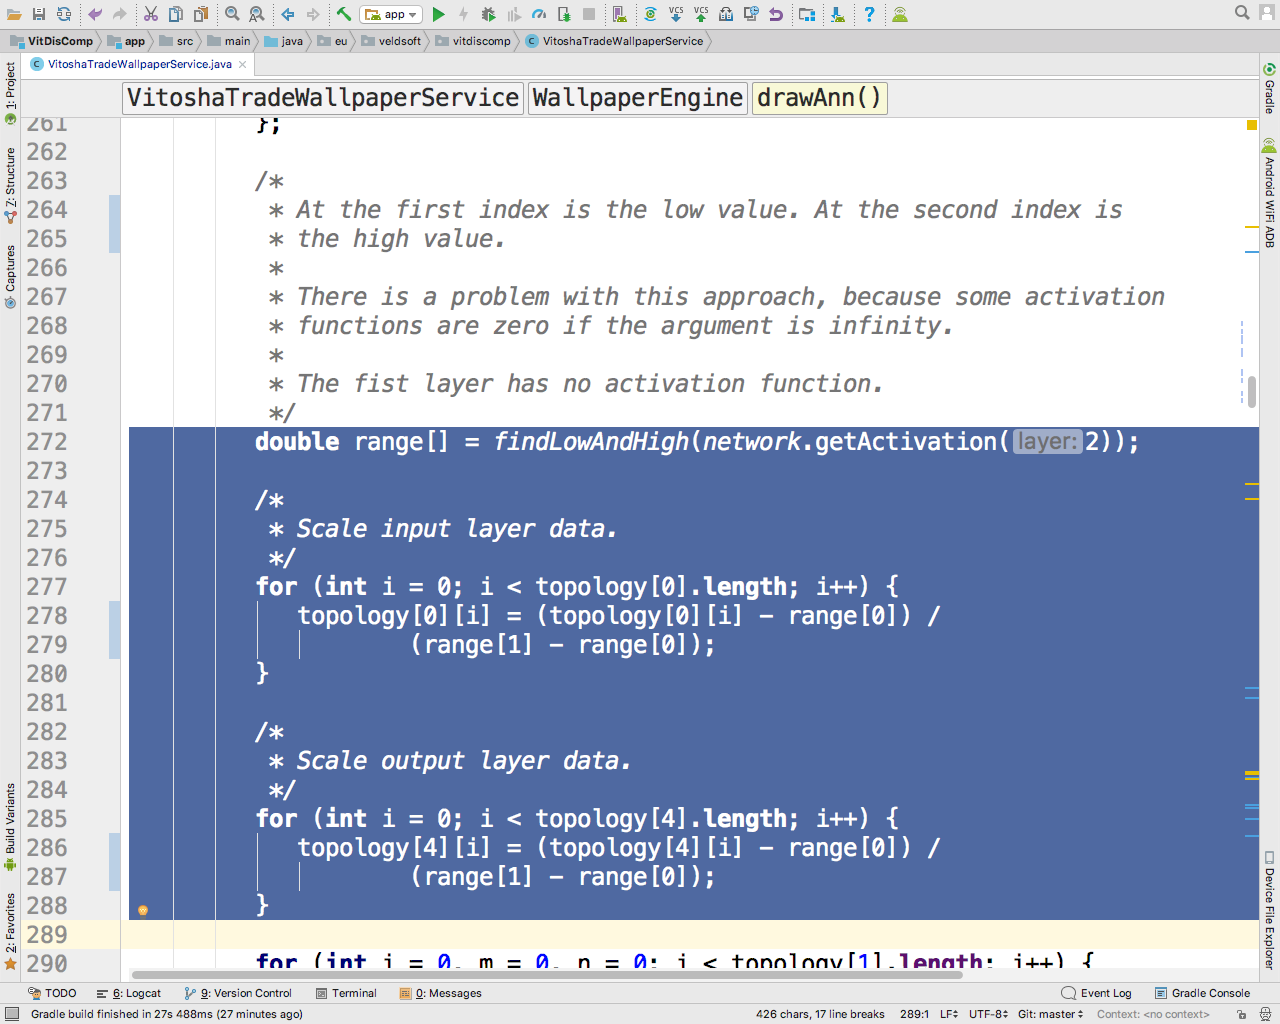
\includegraphics[height=0.45\pdfpageheight]{pic0059}
  \caption{Мащабиране на входната и изходната информация}
\label{fig:pic0059}
\end{figure}
\FloatBarrier

Информацията за входа и изхода се преоразмерява спрямо минималните и максималните стойности с които работят невроните в изходния слой (Фиг. \ref{fig:pic0059}). Невроните във входния слой на практика не би трябвало да имат ограничение от активационна функция, тъй като те само събират информацията от външния свят. 

\begin{figure}[h]
  \centering
  \includegraphics[height=0.45\pdfpageheight]{pic0060}
  \caption{Стойности на теглата между слоевете}
\label{fig:pic0060}
\end{figure}
\FloatBarrier

Следва определянето на теглата между слоевете (Фиг. \ref{fig:pic0060}).

\begin{figure}[h]
  \centering
  \includegraphics[height=0.45\pdfpageheight]{pic0061}
  \caption{Мащабиране на стойностите в скрития слой}
\label{fig:pic0061}
\end{figure}
\FloatBarrier

И финално за средната вертикална област се определят стойностите за скрития слой, мащабирани спрямо минималното и максималното ниво на активационната функция, приложена в него (Фиг. \ref{fig:pic0061}).

\begin{figure}[h]
  \centering
  \includegraphics[height=0.45\pdfpageheight]{pic0062}
  \caption{Нормализиране на стойностите за теглата}
\label{fig:pic0062}
\end{figure}
\FloatBarrier

За да бъде визуализирана информацията за теглата, е нужно стойностите им да се нормализират спрямо най-малката и най-голямата стойност измежду тях (Фиг. \ref{fig:pic0062}).

\begin{figure}[h]
  \centering
  \includegraphics[height=0.45\pdfpageheight]{pic0063}
  \caption{Изрисуване на топологията}
\label{fig:pic0063}
\end{figure}
\FloatBarrier

Така подготвените предварително данни с лекота биват визуализирани от група вложени цикли (Фиг. \ref{fig:pic0063}).

\begin{figure}[h]
  \centering
  \includegraphics[height=0.45\pdfpageheight]{pic0064}
  \caption{Конструктор на двигателя за услугата}
\label{fig:pic0064}
\end{figure}
\FloatBarrier

Конструкторът на двигателя на услугата има единствената задача да зареди нишката за изпълнение (Фиг. \ref{fig:pic0064}).

\begin{figure}[h]
  \centering
  \includegraphics[height=0.45\pdfpageheight]{pic0065}
  \caption{Промяна във видимостта на активния тапет}
\label{fig:pic0065}
\end{figure}
\FloatBarrier

Когато видимостта на активния тапет бъде променена, се активира събитие onVisibilityChanged, в което се определя дали нишката да бъде активирана отново или викането й да бъде преустановено (Фиг. \ref{fig:pic0065}).

\begin{figure}[h]
  \centering
  \includegraphics[height=0.45\pdfpageheight]{pic0066}
  \caption{Спиране на пресмятанията при разрушаване на повърхността за изрисуване}
\label{fig:pic0066}
\end{figure}
\FloatBarrier

При събитие за унищожаване на рисувателната площ, се вдига флаг за спиране на изчисленията и нишката отговорна за тях се премахва от опашката за изпълнение (Фиг. \ref{fig:pic0066}).

\begin{figure}[h]
  \centering
  \includegraphics[height=0.45\pdfpageheight]{pic0067}
  \caption{Размер на зоните за изрисуване}
\label{fig:pic0067}
\end{figure}
\FloatBarrier

Когато настъпи промяна в площта за изрисуване на активния тапет, е нужно да се вземат серия мерки по преизчисляване на размерите. Такова събитие примерно настъпва, когато устройството сменя визуалното представане от портретна в пейзажна или обратното. Първата характеристика която се следи е размерът на петната за визуално представяне (Фиг. \ref{fig:pic0067}).


\begin{figure}[h]
  \centering
  \includegraphics[height=0.45\pdfpageheight]{pic0068}
  \caption{Координати и размери на областите за визуално представяне - горе-ляво}
\label{fig:pic0068}
\end{figure}
\FloatBarrier

\begin{figure}[h]
  \centering
  \includegraphics[height=0.45\pdfpageheight]{pic0069}
  \caption{Координати и размери на областите за визуално представяне - горе-център}
\label{fig:pic0069}
\end{figure}
\FloatBarrier

\begin{figure}[h]
  \centering
  \includegraphics[height=0.45\pdfpageheight]{pic0070}
  \caption{Координати и размери на областите за визуално представяне - горе-дясно}
\label{fig:pic0070}
\end{figure}
\FloatBarrier

\begin{figure}[h]
  \centering
  \includegraphics[height=0.45\pdfpageheight]{pic0071}
  \caption{Координати и размери на областите за визуално представяне - център-ляво}
\label{fig:pic0071}
\end{figure}
\FloatBarrier

\begin{figure}[h]
  \centering
  \includegraphics[height=0.45\pdfpageheight]{pic0072}
  \caption{Координати и размери на областите за визуално представяне - център-център}
\label{fig:pic0072}
\end{figure}
\FloatBarrier

\begin{figure}[h]
  \centering
  \includegraphics[height=0.45\pdfpageheight]{pic0073}
  \caption{Координати и размери на областите за визуално представяне - център-дясно}
\label{fig:pic0073}
\end{figure}
\FloatBarrier

\begin{figure}[h]
  \centering
  \includegraphics[height=0.45\pdfpageheight]{pic0074}
  \caption{Координати и размери на областите за визуално представяне - долу-ляво}
\label{fig:pic0074}
\end{figure}
\FloatBarrier

\begin{figure}[h]
  \centering
  \includegraphics[height=0.45\pdfpageheight]{pic0075}
  \caption{Координати и размери на областите за визуално представяне - долу-център}
\label{fig:pic0075}
\end{figure}
\FloatBarrier

\begin{figure}[h]
  \centering
  \includegraphics[height=0.45\pdfpageheight]{pic0076}
  \caption{Координати и размери на областите за визуално представяне - долу-дясно}
\label{fig:pic0076}
\end{figure}
\FloatBarrier

На потребителя е позволено да избере в коя част на активния тапет да бъдат позиционирани зоните за визуално представяне. Възможностите по хоризонтала са ляво, център и дясно, а възможностите по вертикала са горе, център и долу. 

\begin{figure}[h]
  \centering
  \includegraphics[height=0.45\pdfpageheight]{pic0077}
  \caption{Натоварване на системата за фонови пресмятания}
\label{fig:pic0077}
\end{figure}
\FloatBarrier

Последната характеристика, която потребителят има възможност да контролира, е до каква степен мобилното му устройство да бъде натоварвано с фонови пресмятания (Фиг. \ref{fig:pic0077}).

\section{Представяне на информацията върху локалното устройство}

Ефективността от изчисленията значително се повишава, ако локалните изчислителни възли разполагат с възможност за локално съхранение на изходни данни и пресметнати резултати. 

\begin{figure}[h]
  \centering
  \includegraphics[height=0.45\pdfpageheight]{pic0078}
  \caption{Константи за интервалите на времевия ред (0 до 15)}
\label{fig:pic0078}
\end{figure}
\FloatBarrier

За нуждите на това локално представяне се ползва помощен тип данни от изброен тип, който обозначава разстоянието между две отчитания във финансовите времеви редове (Фиг. \ref{fig:pic0078}, \ref{fig:pic0079}).

\begin{figure}[h]
  \centering
  \includegraphics[height=0.45\pdfpageheight]{pic0079}
  \caption{Константи за интервалите на времевия ред (30 до 43200)}
\label{fig:pic0079}
\end{figure}
\FloatBarrier

Интервалите в използваните времеви редове се определят на база брой минути като най-краткият интервал е една минута. Описването на интервалите става с две променливи - название и брой минути (Фиг. \ref{fig:pic0080}).

\begin{figure}[h]
  \centering
  \includegraphics[height=0.45\pdfpageheight]{pic0080}
  \caption{Описание на времеви интервал}
\label{fig:pic0080}
\end{figure}
\FloatBarrier

Използването на изброени константи в Java дава възможност за елегантно използване на статични функции за конструиране на обекти (Factory Method Design Pattern), които по зададено число (брой минути) да връщат съответстващата константа (Фиг. \ref{fig:pic0081}).

\begin{figure}[h]
  \centering
  \includegraphics[height=0.45\pdfpageheight]{pic0081}
  \caption{Определяне на константа за интервал по брой минути}
\label{fig:pic0081}
\end{figure}
\FloatBarrier

Аналогичен ефект може да се постигне и с използване на текстовото описание на константите (Фиг. \ref{fig:pic0082}).

\begin{figure}[h]
  \centering
  \includegraphics[height=0.45\pdfpageheight]{pic0082}
  \caption{Определяне на константа за интервал по текстово описание}
\label{fig:pic0082}
\end{figure}
\FloatBarrier

За да се възпрепятства създаването на константи извън изброения тип, е прието конструкторът да бъде с частно ниво на достъп (Фиг. \ref{fig:pic0083}).

\begin{figure}[h]
  \centering
  \includegraphics[height=0.45\pdfpageheight]{pic0083}
  \caption{Конструктор на изброения тип за интервал}
\label{fig:pic0083}
\end{figure}
\FloatBarrier

Операционната система Android предоставя изключително полезни средства за съхраняване на информация, едно от които е релационната система за управление на бази от данни SQLite. 

\begin{figure}[h]
  \centering
  \includegraphics[height=0.45\pdfpageheight]{pic0084}
  \caption{Структура на локалната таблица за котировките}
\label{fig:pic0084}
\end{figure}
\FloatBarrier

Информацията за времевия ред може да се съхранява локално в таблица с подходяща структура, която да отразява наличието на четири стойности за всеки интервал, времето на интервала, търгувания обем, названието на валутната двойка и размера на времевия интервал (Фиг. \ref{fig:pic0084}).

\begin{figure}[h]
  \centering
  \includegraphics[height=0.45\pdfpageheight]{pic0085}
  \caption{Структура на локалната таблица за изкуствените невронни мрежи}
\label{fig:pic0085}
\end{figure}
\FloatBarrier

Допълнителна таблица поема съхранението на информацията за изкуствените неврони мрежи, което включва названието на валутната двойка, времевия интервал, стойността на невроните, стойността на връзките между невроните и стойността на теглата между невроните (Фиг. \ref{fig:pic0085}). 

\begin{figure}[h]
  \centering
  \includegraphics[height=0.45\pdfpageheight]{pic0086}
  \caption{Име и версията на базата данни}
\label{fig:pic0086}
\end{figure}
\FloatBarrier

Android управлява базите от данни под формата на DB ресурс и целочислена версия за структурата (Фиг. \ref{fig:pic0086}).

\begin{figure}[h]
  \centering
  \includegraphics[height=0.45\pdfpageheight]{pic0087}
  \caption{Код за създаване на таблицата за котировки}
\label{fig:pic0087}
\end{figure}
\FloatBarrier

\begin{figure}[h]
  \centering
  \includegraphics[height=0.45\pdfpageheight]{pic0088}
  \caption{Код за създаване на таблицата за изкуствените невронни мрежи}
\label{fig:pic0088}
\end{figure}
\FloatBarrier

Създаването на таблиците се управлява от параметризирани символни константи (Фиг. \ref{fig:pic0087}, \ref{fig:pic0088}).

\begin{figure}[h]
  \centering
  \includegraphics[height=0.45\pdfpageheight]{pic0089}
  \caption{Код за изтриване на таблиците}
\label{fig:pic0089}
\end{figure}
\FloatBarrier

Изтриването на таблиците също става с параметризирани символни константи (Фиг. \ref{fig:pic0089}).

\begin{figure}[h]
  \centering
  \includegraphics[height=0.45\pdfpageheight]{pic0090}
  \caption{Конструктор и виртуални методи на спомагателния клас за базата данни}
\label{fig:pic0090}
\end{figure}
\FloatBarrier

Конструкторът на спомагателния клас за базата данни има единствена задача да извика конструкторът на родителския клас (Фиг. \ref{fig:pic0090}). Двете предефинирани виртуални функции имат за задача да извикат заявките за конструиране и обновяване на базата данни (Фиг. \ref{fig:pic0090}). 

\begin{figure}[h]
  \centering
  \includegraphics[height=0.45\pdfpageheight]{pic0091}
  \caption{Изброен тип за вида на невроните}
\label{fig:pic0091}
\end{figure}
\FloatBarrier

Вторият изброен тип данни е по отношение на типа неврони. В общия случай невроните могат да бъдат обикновени, входни, изходни и отместващи (bias) (Фиг. \ref{fig:pic0090}).

\begin{figure}[h]
  \centering
  \includegraphics[height=0.45\pdfpageheight]{pic0092}
  \caption{Целочислена константа за типа на неврона, която може да се ползва и като битово поле}
\label{fig:pic0092}
\end{figure}
\FloatBarrier

Тъй като са възможни различни връзки между невроните, то се появяват и неврони с повече функции като: обикновен-входен, обикновен-изходен, входен-изходен, входен-обикновен-изходен. Всички възможни комбинации се записват в целочислена променлива, която може да послужи и като битово поле (Фиг. \ref{fig:pic0092}).

\begin{figure}[h]
  \centering
  \includegraphics[height=0.45\pdfpageheight]{pic0093}
  \caption{Определяне на изброимата константа по числена стойност}
\label{fig:pic0093}
\end{figure}
\FloatBarrier

Тъй като информацията от сървъра пристига предимно под формата на числа, то е рационално да бъде добавена статичена функция за конструиране на обекта (Factory Method Design Pattern), която по числена стойност да определя константата в изброения тип (Фиг. \ref{fig:pic0093}).

\begin{figure}[h]
  \centering
  \includegraphics[height=0.45\pdfpageheight]{pic0094}
  \caption{Методи за достъп до вътрешните стойности на константите}
\label{fig:pic0094}
\end{figure}
\FloatBarrier

За удобство, при работата с константите и със скритата в тях информация, често се използват методи за достъп (accessor). В този случай един публичен getter, но setter с частен достъп. Разумно е setter-ът да бъде с частен достъп, тъй като е разумно да се запази свойството на изброените константи да бъдат константи (Фиг. \ref{fig:pic0094}).